%% Volume I, Chapter 3: Number Systems
\chapter{Number Systems}
\label{ch:numbers}

\abstract{A computer does not calculate with integers or real numbers. It calculates with patterns of $64$ bits, which imitate a finite part of $\mathbb Z$, and with floating-point numbers, which imitate a finite part of $\mathbb R$. The imitations are good but not perfect: adding $1$ to the largest integer of a machine can produce a negative number, and the number $0.1$ cannot be stored exactly. To see where and why an imitation departs from the original, we must first know precisely what the original guarantees. This chapter builds the number systems from the natural numbers up to the complex numbers and collects the facts about divisibility, remainders, digits and inequalities on which the later volumes rely.}

The first two chapters used the numbers freely. \Cref{ch:logic} listed the properties of $\mathbb N$, $\mathbb Z$, $\mathbb Q$ and $\mathbb R$ that it needed in \cref{asm:numbers} and took them for granted, and \cref{ch:sets} added a few more promises: that every integer leaves a unique remainder on division by a positive integer, that the greatest common divisor and the least common multiple exist and behave as expected, that between two real numbers there is always a rational number, and that the real numbers are characterised by the completeness axiom. This chapter keeps these promises. It also proves the facts about the integers that the later volumes need most often: the Euclidean algorithm, unique factorisation into primes, arithmetic modulo $n$ and the representation of numbers by digits in a base.

The chapter climbs a ladder. \Cref{sec:naturals} starts from Peano's axioms for the natural numbers, which say little more than that one can count from $0$ by adding $1$ and that induction works. \Cref{sec:integers} constructs the integers from pairs of natural numbers, so that subtraction becomes possible. \Cref{sec:division,sec:gcd,sec:primes,sec:congruences,sec:positional} stay with the integers and study division: remainders, greatest common divisors, primes, congruences and positional notation. \Cref{sec:rationals} constructs the rational numbers from pairs of integers, so that division becomes possible, and shows that the rational number line has gaps. \Cref{sec:reals} fills the gaps by the completeness axiom and derives the properties of the real numbers that calculus uses, and \cref{sec:complex} adds a square root of $-1$. The last section, \cref{sec:inequalities}, collects the inequalities that error bounds in later volumes are made of.

At every rung the same question arises: which properties survive the passage to the next system, and which are lost? The integers can be subtracted but not divided; the rational numbers can be divided but have gaps; the real numbers have no gaps but no square root of $-1$; the complex numbers have every square root but can no longer be ordered. Computer arithmetic has its own answers to the same question, and we point them out as we go. This is a review chapter: every result is stated precisely, the important ones are proved, and for the others we describe the idea of the proof and give a reference.

\section{The Natural Numbers}
\label{sec:naturals}

What is the number $3$? It is what the sets $\{a,b,c\}$, $\{0,1,2\}$ and $\{\text{red},\text{green},\text{blue}\}$ have in common, the result of counting ``zero, one, two, three''. Counting has a simple structure: there is a first number, and every number has a next one. Richard Dedekind~\cite{dedekind1888} and Giuseppe Peano~\cite{peano1889} showed that this structure, together with the principle of induction, characterises the natural numbers completely. Everything else, addition and multiplication included, can be defined from it.

\subsection{Peano's Axioms}

\begin{definition}[Peano system]
\label{def:peano}
A \term{Peano system} consists of a set $N$, an element $0\in N$ and a function $S\colon N\to N$, the \term{successor function}, such that
\begin{enumerate}
\item $0$ is not a successor: $S(n)\ne0$ for every $n\in N$;
\item different elements have different successors: $S$ is injective;
\item every subset $A\subseteq N$ that contains $0$ and contains $S(n)$ whenever it contains $n$ is the whole of $N$.
\end{enumerate}
\end{definition}

The three conditions are known as \term{Peano's axioms}. Condition (iii) is the axiom of induction. If $P(n)$ is a predicate on $N$ such that $P(0)$ holds and $P(n)$ implies $P(S(n))$, then its truth set $A=\{n\in N: P(n)\}$ satisfies the hypothesis of (iii), so $A=N$ and $P(n)$ holds for every $n$. This is the principle of induction that \cref{ch:logic} adopted as \cref{asm:induction}.

\begin{assumption}[The natural numbers]
\label{asm:peano}
There is a Peano system. We fix one, denote its set by $\mathbb N$, and call its elements the \term{natural numbers}. We write $1\coloneqq S(0)$, $2\coloneqq S(1)$, $3\coloneqq S(2)$, and so on.
\end{assumption}

Each axiom excludes a way in which a ``counting structure'' could go wrong, and \cref{fig:peano} shows the possibilities. Axiom (i) excludes counting in a circle, where the successor of the last element is $0$ again. Axiom (ii) excludes a chain that runs for a while and then joins an earlier part of itself, so that some element is the successor of two different elements. Axiom (iii) excludes extra elements that cannot be reached from $0$ by counting, such as a second chain beside the first. What is left is the single endless chain $0\to1\to2\to\cdots$ of panel~A.

\begin{figure}
\tikzset{pd/.style={circle, fill=black, inner sep=0pt, minimum size=3.2pt},
  pa/.style={-{Latex[length=1.3mm]}, line width=0.4pt, shorten >=1.6pt, shorten <=1.6pt}}
\sdpanel{A}{\begin{tikzpicture}[font=\scriptsize]
\foreach \i in {0,...,6} {\node[pd] (n\i) at (\i*0.85,0) {}; \node[below=1pt] at (n\i) {$\i$};}
\foreach \i [count=\j] in {0,...,5} {\draw[pa] (n\i) -- (n\j);}
\node (dots) at (5.8,0) {$\cdots$};
\draw[pa] (n6) -- (dots);
\end{tikzpicture}}
\sdpanelrow
\sdpanel{B}{\begin{tikzpicture}[font=\scriptsize]
\foreach \i in {0,...,7} {\node[pd] (c\i) at ({90-45*\i}:0.95) {}; \node at ({90-45*\i}:1.25) {$\i$};}
\foreach \i [evaluate=\i as \j using {int(mod(\i+1,8))}] in {0,...,7} {\draw[pa] (c\i) to[bend left=12] (c\j);}
\end{tikzpicture}}\hfill
\sdpanel{C}{\begin{tikzpicture}[font=\scriptsize]
\node[pd] (r0) at (0,0) {}; \node[below=1pt] at (r0) {$0$};
\node[pd] (r1) at (0.85,0) {}; \node[below=1pt] at (r1) {$1$};
\node[pd] (r2) at (1.7,0) {}; \node[below=1pt] at (r2) {$2$};
\node[pd] (r3) at (2.45,0.55) {}; \node[right=1pt] at (r3) {$3$};
\node[pd] (r4) at (2.05,1.3) {}; \node[above=1pt] at (r4) {$4$};
\node[pd] (r5) at (1.25,1.05) {}; \node[left=1pt] at (r5) {$5$};
\draw[pa] (r0) -- (r1); \draw[pa] (r1) -- (r2); \draw[pa] (r2) -- (r3);
\draw[pa] (r3) -- (r4); \draw[pa] (r4) -- (r5); \draw[pa] (r5) -- (r2);
\path (0,-0.62) -- (0,1.6);
\end{tikzpicture}}\hfill
\sdpanel{D}{\begin{tikzpicture}[font=\scriptsize]
\foreach \i in {0,...,3} {\node[pd] (d\i) at (\i*0.8,0.75) {}; \node[above=1pt] at (d\i) {$\i$};}
\foreach \i [count=\j] in {0,...,2} {\draw[pa] (d\i) -- (d\j);}
\node (dd) at (3.15,0.75) {$\cdots$}; \draw[pa] (d3) -- (dd);
\node (el) at (-0.45,0) {$\cdots$};
\foreach \l [count=\i] in {a,b,c,d} {\node[pd] (e\i) at (\i*0.8-0.4,0) {}; \node[below=1pt] at (e\i) {$\l$};}
\draw[pa] (el) -- (e1);
\foreach \i [count=\j from 2] in {1,...,3} {\draw[pa] (e\i) -- (e\j);}
\node (er) at (3.55,0) {$\cdots$}; \draw[pa] (e4) -- (er);
\path (0,-0.62) -- (0,1.6);
\end{tikzpicture}}
\caption{Peano's axioms. An arrow points from each element to its successor. (A) The natural numbers: a single chain starting at $0$. (B) A cycle of eight elements violates axiom (i), since $0$ is the successor of $7$; unsigned $3$-bit machine integers behave in this way. (C) A chain that runs into itself violates axiom (ii), since $2$ is the successor of both $1$ and $5$. (D) The natural numbers together with a second, two-sided chain satisfy (i) and (ii) but violate the axiom of induction: the upper chain contains $0$ and is closed under successors without being everything.}
\label{fig:peano}
\end{figure}

Panel B is not an academic curiosity. An unsigned integer of $k$ bits in a computer holds the values $0,1,\ldots,2^k-1$, and adding $1$ to the largest of them gives $0$: the carry out of the highest bit is discarded. The machine integers therefore form a cycle like that of panel~B, with $2^k$ elements instead of eight, and they violate the first of Peano's axioms. \Cref{sec:congruences} identifies the structure they do have.

Two simple consequences of the axioms are used constantly.

\begin{proposition}
\label{prop:peano-basic}
\leavevmode
\begin{enumerate}
\item Every natural number $n\ne0$ is a successor: $n=S(m)$ for exactly one $m\in\mathbb N$.
\item $S(n)\ne n$ for every $n\in\mathbb N$.
\end{enumerate}
\end{proposition}

\begin{proof}
(i) The set $A\coloneqq\{0\}\cup S(\mathbb N)$ contains $0$, and it contains $S(n)$ for every $n\in\mathbb N$, in particular for every $n\in A$. By axiom (iii), $A=\mathbb N$, so every $n\ne0$ lies in $S(\mathbb N)$. The element $m$ is unique by axiom (ii).

(ii) By induction on $n$. We have $S(0)\ne0$ by axiom (i). If $S(n)\ne n$, then $S(S(n))\ne S(n)$, because $S$ is injective.
\end{proof}

\subsection{Definition by Recursion}

\Cref{ch:logic} defined sums and powers recursively: the first value is given, and each further value is given in terms of the previous one. The axioms guarantee that such definitions really define a function~\cite{dedekind1888}.

\begin{theorem}[Recursion theorem]
\label{thm:recursion}
Let $X$ be a set, $a\in X$ and $g\colon X\to X$ a function. There is exactly one function $f\colon\mathbb N\to X$ such that
\[
f(0)=a\qquad\text{and}\qquad f(S(n))=g(f(n))\quad\text{for every }n\in\mathbb N.
\]
\end{theorem}

\begin{proof}
\emph{Uniqueness.} If $f$ and $f'$ both have the two properties, then $f(0)=a=f'(0)$, and $f(n)=f'(n)$ implies $f(S(n))=g(f(n))=g(f'(n))=f'(S(n))$. By induction, $f(n)=f'(n)$ for all $n$.

\emph{Existence.} The function is built from its graph. Call a set $R\subseteq\mathbb N\times X$ \emph{admissible} if $(0,a)\in R$ and $(n,x)\in R$ implies $(S(n),g(x))\in R$; the set $\mathbb N\times X$ itself is admissible. Let $F$ be the intersection of all admissible sets. Then $F$ is admissible, and it is the smallest admissible set, as in the construction of the transitive closure in \cref{prop:transitive-closure}. One shows by induction on $n$ that for each $n$ there is exactly one $x$ with $(n,x)\in F$. That there is at least one follows by induction from admissibility. If there were a second pair, removing it from $F$ would leave a set that is still admissible, contradicting minimality. For $n=0$ this holds because $0$ is not a successor (axiom (i)), so admissibility never forces a pair $(0,y)$ with $y\ne a$. In the inductive step a pair $(S(n),y)$ with $y\ne g(x)$, where $x$ is the unique value paired with $n$, is never forced either, because $S(m)=S(n)$ only for $m=n$ (axiom (ii)). Hence $F$ is the graph of a function $f$, and admissibility says precisely that $f(0)=a$ and $f(S(n))=g(f(n))$. Complete proofs are given by Enderton~\cite{enderton1977sets} and by Hrbacek and Jech~\cite{hrbacek1999}.
\end{proof}

The theorem is less obvious than it looks, and the axioms are needed for it. On the cycle of \cref{fig:peano}B, for instance, the ``definition'' $f(0)=0$, $f(S(n))=f(n)+1$ with values in $\mathbb N$ would require $f(0)=f(S(7))=f(7)+1=8$, which contradicts $f(0)=0$. A useful variant allows $g$ to depend on $n$ as well: there is exactly one $f$ with $f(0)=a$ and $f(S(n))=g(n,f(n))$ for a given function $g\colon\mathbb N\times X\to X$. It is proved in the same way, and it covers definitions such as $0!\coloneqq1$, $(n+1)!\coloneqq(n+1)\cdot n!$.

The recursion theorem also shows that Peano's axioms leave no freedom: any two Peano systems are copies of each other, so that it does not matter which one \cref{asm:peano} fixes.

\begin{proposition}[Dedekind]
\label{prop:peano-unique}
Let $(N,0,S)$ and $(N',0',S')$ be Peano systems. There is exactly one bijection $\varphi\colon N\to N'$ with $\varphi(0)=0'$ and $\varphi(S(n))=S'(\varphi(n))$ for every $n\in N$.
\end{proposition}

\begin{proof}
The recursion theorem for the system $(N,0,S)$, applied with $X=N'$, $a=0'$ and $g=S'$, gives exactly one function $\varphi$ with the two properties. Applied to the system $(N',0',S')$ with $X=N$, it gives a function $\psi\colon N'\to N$ with $\psi(0')=0$ and $\psi(S'(n'))=S(\psi(n'))$. The composition $\psi\circ\varphi\colon N\to N$ satisfies $(\psi\circ\varphi)(0)=0$ and $(\psi\circ\varphi)(S(n))=S\bigl((\psi\circ\varphi)(n)\bigr)$, and so does the identity function of $N$. By the uniqueness part of \cref{thm:recursion}, $\psi\circ\varphi=\operatorname{id}_N$. In the same way $\varphi\circ\psi=\operatorname{id}_{N'}$, so $\varphi$ is a bijection by \cref{thm:inverse}.
\end{proof}

\subsection{Addition and Multiplication}

With recursion available, the arithmetic operations can be defined. Fix $m\in\mathbb N$. Addition of $m$ is defined by recursion on the second argument,
\begin{equation}
m+0\coloneqq m,\qquad m+S(n)\coloneqq S(m+n),
\label{eq:peano-add}
\end{equation}
and multiplication by
\begin{equation}
m\cdot0\coloneqq0,\qquad m\cdot S(n)\coloneqq m\cdot n+m .
\label{eq:peano-mul}
\end{equation}
In words: adding the successor of $n$ means adding $n$ and then counting one further, and multiplying by the successor of $n$ means multiplying by $n$ and then adding one more copy of $m$. The first rule gives $m+1=m+S(0)=S(m+0)=S(m)$, so the successor of $m$ is $m+1$, and from now on we write $n+1$ instead of $S(n)$. A small computation shows how the definitions work:
\[
2+2=2+S(1)=S(2+1)=S\bigl(2+S(0)\bigr)=S\bigl(S(2+0)\bigr)=S(S(2))=S(3)=4 .
\]
Powers are defined in the same way by $m^0\coloneqq1$ and $m^{n+1}\coloneqq m^n\cdot m$. All the familiar laws of arithmetic follow from these definitions by induction.

\begin{theorem}[Arithmetic of the natural numbers]
\label{thm:n-arith}
For all $k,m,n\in\mathbb N$:
\begin{enumerate}
\item $(k+m)+n=k+(m+n)$ and $(km)n=k(mn)$ (associative laws);
\item $m+n=n+m$ and $mn=nm$ (commutative laws);
\item $m+0=m$ and $m\cdot1=m$ (neutral elements);
\item $k(m+n)=km+kn$ (distributive law);
\item if $m+k=n+k$, then $m=n$ (cancellation);
\item if $m+n=0$, then $m=n=0$; if $mn=0$, then $m=0$ or $n=0$.
\end{enumerate}
\end{theorem}

\begin{proof}
We prove the associative law of addition, the commutative law of addition and the cancellation law. The others are proved by similar inductions on one of the variables. For the laws of multiplication, the distributive law $k(m+n)=km+kn$ comes first, by induction on $n$; the associative law follows from it, and the commutative law, like that of addition, needs the two auxiliary rules $0\cdot n=0$ and $S(m)\cdot n=mn+n$. Part (vi) follows from \cref{prop:peano-basic}\,(i): if $n\ne0$, then $n=S(j)$, so $m+n=S(m+j)\ne0$, and $mn=mj+m\ne0$ when also $m\ne0$. Landau carries out all these proofs in full~\cite{landau1930}, with the minor difference that his natural numbers start at $1$.

\emph{Associativity of addition.} Fix $k$ and $m$, and use induction on $n$. For $n=0$, both sides equal $k+m$ by \eqref{eq:peano-add}. Suppose $(k+m)+n=k+(m+n)$. Then, using \eqref{eq:peano-add} three times and the inductive hypothesis once,
\[
(k+m)+S(n)=S\bigl((k+m)+n\bigr)=S\bigl(k+(m+n)\bigr)=k+S(m+n)=k+\bigl(m+S(n)\bigr).
\]

\emph{Commutativity of addition.} We first prove two special cases by induction on $n$. (a) $0+n=n$: true for $n=0$, and $0+n=n$ implies $0+S(n)=S(0+n)=S(n)$. (b) $S(m)+n=S(m+n)$: true for $n=0$, since both sides equal $S(m)$, and if it holds for $n$, then $S(m)+S(n)=S\bigl(S(m)+n\bigr)=S\bigl(S(m+n)\bigr)=S\bigl(m+S(n)\bigr)$. Now fix $n$ and use induction on $m$. For $m=0$, $0+n=n=n+0$ by (a). If $m+n=n+m$, then by (b) and \eqref{eq:peano-add}, $S(m)+n=S(m+n)=S(n+m)=n+S(m)$.

\emph{Cancellation.} By induction on $k$. For $k=0$ there is nothing to prove. If the law holds for $k$ and $m+S(k)=n+S(k)$, then $S(m+k)=S(n+k)$, so $m+k=n+k$ by axiom (ii), and $m=n$ by the inductive hypothesis.
\end{proof}

The proof of commutativity deserves a second look: the law that every child knows from counting objects in two different orders requires two auxiliary inductions when only the successor function is available. This is the price of starting from so little, and the reward is that nothing has been assumed that could turn out to be false.

\subsection{Order}

\begin{definition}[Order of the natural numbers]
\label{def:n-order}
For $m,n\in\mathbb N$ we write $m\le n$ if there is $k\in\mathbb N$ with $n=m+k$, and $m<n$ if $m\le n$ and $m\ne n$.
\end{definition}

The number $k$ in the definition is unique by the cancellation law; it is the difference $n-m$, which is so far defined only when $m\le n$.

\begin{theorem}[Order of the natural numbers]
\label{thm:n-order}
\leavevmode
\begin{enumerate}
\item The relation $\le$ is a total order on $\mathbb N$, and $0$ is its least element.
\item $m<n$ if and only if $m+1\le n$. In particular, there is no natural number strictly between $n$ and $n+1$.
\item If $m\le n$, then $m+k\le n+k$ and $mk\le nk$ for every $k\in\mathbb N$.
\item Every nonempty subset of $\mathbb N$ has a least element.
\end{enumerate}
\end{theorem}

\begin{proof}
(i) Reflexivity: $n=n+0$. Transitivity: if $n=m+k$ and $p=n+l$, then $p=m+(k+l)$. Antisymmetry: if $n=m+k$ and $m=n+l$, then $m+0=m=m+(k+l)$, so $k+l=0$ by cancellation, and $k=l=0$ by \cref{thm:n-arith}\,(vi); thus $m=n$. The number $0$ is least because $n=0+n$. Totality is proved by induction on $m$, the statement being ``$m\le n$ or $n\le m$, for every $n$''. For $m=0$ this holds because $0$ is least. Suppose it holds for $m$, and let $n\in\mathbb N$. If $n\le m$, then $n\le m+1$, since $m\le m+1$. Otherwise $m<n$, and then $m+1\le n$ by (ii), whose proof does not use totality.

(ii) If $m<n$, then $n=m+k$ with $k\ne0$, so $k=j+1$ for some $j$ by \cref{prop:peano-basic}\,(i), and $n=(m+1)+j$. Conversely, if $n=(m+1)+j$, then $n=m+(j+1)$ with $j+1\ne0$, so $m\le n$, and $m\ne n$ because $m=m+(j+1)$ would give $j+1=0$ by cancellation.

(iii) If $n=m+j$, then $n+k=(m+k)+j$ and $nk=mk+jk$.

(iv) This is the well-ordering principle, \cref{thm:well-ordering}. Its proof in \cref{ch:logic} used strong induction (\cref{thm:strong-induction}), which follows from ordinary induction, together with the facts that $0$ is the least natural number, that the order is total and that $m<n$ implies $m+1\le n$. These are (i) and (ii), so the principle now rests on Peano's axioms alone.
\end{proof}

From here on, the natural numbers have all the properties used in \cref{ch:logic} that concern addition, multiplication and order alone. What they lack is subtraction: the equation $m+x=n$ has a solution $x\in\mathbb N$ only when $m\le n$.

\begin{note}{Natural numbers as sets}
In axiomatic set theory (see the note in \cref{sec:sets}) a Peano system is constructed rather than assumed. Following John von Neumann, one puts $0\coloneqq\emptyset$ and $S(n)\coloneqq n\cup\{n\}$, so that
\[
1=\{0\},\qquad2=\{0,1\},\qquad3=\{0,1,2\},\qquad\ldots,
\]
and each natural number is the set of its predecessors. The axiom of infinity provides a set that contains $\emptyset$ and is closed under $S$; the intersection of all such subsets of it is the set $\mathbb N$, and Peano's axioms become theorems~\cite{enderton1977sets,hrbacek1999}. In this model $m<n$ means $m\in n$, and a set has $n$ elements in the sense of \cref{def:finite} exactly when it is in bijection with the set $n$ itself. By \cref{prop:peano-unique}, every other construction yields a copy of the same structure, which is why mathematicians can speak of ``the'' natural numbers without committing to any construction.
\end{note}

\section{The Integers}
\label{sec:integers}

To make subtraction always possible, we add the negative numbers. Rather than adding them by decree, we construct them from what we have, using the quotient sets of \cref{sec:equivalence}. The idea is that every integer is a difference $a-b$ of two natural numbers, and that two differences $a-b$ and $c-d$ are equal exactly when $a+d=b+c$, a condition that mentions only addition.

\subsection{Construction}

\begin{lemma}
\label{lem:z-equivalence}
The relation on $\mathbb N\times\mathbb N$ defined by
\[
(a,b)\sim(c,d)\iff a+d=b+c
\]
is an equivalence relation.
\end{lemma}

\begin{proof}
Reflexivity and symmetry follow from the commutative law of addition. For transitivity, suppose $a+d=b+c$ and $c+f=d+e$. Adding the two equations gives $a+d+c+f=b+c+d+e$, and cancelling $c+d$ (\cref{thm:n-arith}\,(v)) leaves $a+f=b+e$, that is, $(a,b)\sim(e,f)$.
\end{proof}

\begin{definition}[Integers]
\label{def:integers}
The set of \term{integers} is the quotient set $\mathbb Z\coloneqq(\mathbb N\times\mathbb N)/{\sim}$. Addition and multiplication of classes are defined by
\[
[(a,b)]+[(c,d)]\coloneqq[(a+c,\,b+d)],\qquad
[(a,b)]\cdot[(c,d)]\coloneqq[(ac+bd,\,ad+bc)].
\]
\end{definition}

The formulas are what the rules of algebra predict if $[(a,b)]$ stands for $a-b$: $(a-b)+(c-d)=(a+c)-(b+d)$ and $(a-b)(c-d)=(ac+bd)-(ad+bc)$. \Cref{fig:integers} shows the classes. They are the diagonal lines of the grid $\mathbb N\times\mathbb N$, and each line corresponds to one integer, the common value of $a-b$ along it.

\begin{figure}
\sdfloat{%
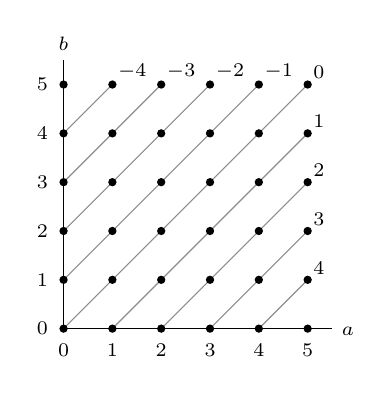
\begin{tikzpicture}[font=\scriptsize, x=0.62cm, y=0.62cm]
\foreach \k in {-4,...,4} {
  \pgfmathsetmacro\xs{max(0,\k)}
  \pgfmathsetmacro\ys{max(0,-\k)}
  \pgfmathsetmacro\xe{min(5,5+\k)}
  \pgfmathsetmacro\ye{min(5,5-\k)}
  \draw[black!45, line width=0.4pt] (\xs,\ys) -- (\xe,\ye);}
\draw[line width=0.4pt] (0,0) -- (5.5,0); \draw[line width=0.4pt] (0,0) -- (0,5.5);
\foreach \i in {0,...,5} {\node[below] at (\i,-0.12) {$\i$}; \node[left] at (-0.12,\i) {$\i$};}
\foreach \a in {0,...,5} \foreach \b in {0,...,5} {\fill (\a,\b) circle (1.5pt);}
\foreach \k in {-4,...,-1} {\pgfmathtruncatemacro\yy{5+\k}\node[anchor=south west, inner sep=1pt] at (\yy+0.05,5.05) {$\k$};}
\foreach \k in {0,...,4} {\pgfmathtruncatemacro\yy{5-\k}\node[anchor=south west, inner sep=1pt] at (5.05,\yy+0.05) {$\k$};}
\node[anchor=west] at (5.5,-0.05) {$a$};
\node[anchor=south] at (0,5.5) {$b$};
\end{tikzpicture}}{The integers as classes of pairs. A pair $(a,b)$ of natural numbers stands for the difference $a-b$; the pairs on one diagonal line form one equivalence class, labelled at the end of the line by its integer value. The class of $0$ is the main diagonal, the classes of the positive integers lie below it and those of the negative integers above it.\label{fig:integers}}
\end{figure}

Since a class has many representatives, we must check that the definitions do not depend on the choice, as explained in \cref{sec:equivalence}.

\begin{proposition}
\label{prop:z-well-defined}
Addition and multiplication of integers are well defined.
\end{proposition}

\begin{proof}
Let $(a,b)\sim(a',b')$, that is, $a+b'=b+a'$, and let $(c,d)$ be any pair. For addition, $(a+c)+(b'+d)=(b+d)+(a'+c)$ follows by adding $c+d$ to both sides of $a+b'=b+a'$, so $(a+c,b+d)\sim(a'+c,b'+d)$. For multiplication we must show
\[
(ac+bd)+(a'd+b'c)=(ad+bc)+(a'c+b'd).
\]
Multiplying $a+b'=b+a'$ by $c$ gives $ac+b'c=bc+a'c$, and multiplying it by $d$ gives $ad+b'd=bd+a'd$. Adding the first equation to the second, read from right to left, gives exactly the required identity. So the result does not change when the first factor is replaced by an equivalent pair; by the commutativity of the formulas, the same holds for the second factor, and replacing both factors one after the other shows that the operations are well defined.
\end{proof}

The natural numbers sit inside $\mathbb Z$ through the map $n\mapsto[(n,0)]$. It is injective, because $(m,0)\sim(n,0)$ means $m=n$, and it respects the operations: $[(m,0)]+[(n,0)]=[(m+n,0)]$ and $[(m,0)]\cdot[(n,0)]=[(mn,0)]$. We therefore identify $n$ with $[(n,0)]$ and regard $\mathbb N$ as a subset of $\mathbb Z$. The \term{negative} of $x=[(a,b)]$ is $-x\coloneqq[(b,a)]$; it satisfies $x+(-x)=[(a+b,a+b)]=[(0,0)]=0$. With subtraction defined by $x-y\coloneqq x+(-y)$, we get $[(a,b)]=[(a,0)]+[(0,b)]=a-b$, as intended.

\begin{proposition}
\label{prop:z-sign}
Every integer is either a natural number $n$ or the negative $-n$ of a natural number $n\ge1$, and not both.
\end{proposition}

\begin{proof}
Let $x=[(a,b)]$. By \cref{thm:n-order}\,(i), $b\le a$ or $a<b$. If $b\le a$, say $a=b+n$, then $(a,b)\sim(n,0)$, so $x=n$. If $a<b$, say $b=a+n$ with $n\ge1$, then $(a,b)\sim(0,n)$, so $x=-n$. A natural number $m$ cannot equal $-n$ with $n\ge1$, since $(m,0)\sim(0,n)$ would mean $m+n=0$, which forces $n=0$.
\end{proof}

So $\mathbb Z=\{\ldots,-2,-1,0,1,2,\ldots\}$, as we have always written it, and every equation $m+x=n$ with $m,n\in\mathbb Z$ now has exactly one solution $x=n-m$. The construction has done its job.

\subsection{Rings}

The laws of arithmetic that $\mathbb Z$ satisfies are shared by many other systems in this series: the rational, real and complex numbers, the integers modulo $n$ of \cref{sec:congruences}, polynomials, and square matrices (although the last are not commutative). It pays to name them once.

\begin{definition}[Commutative ring, field]
\label{def:ring}
A \term{commutative ring} is a set $R$ with two operations, addition $(a,b)\mapsto a+b$ and multiplication $(a,b)\mapsto ab$, and two elements $0$ and $1$, that satisfy the axioms A1--A4, M1--M3 and D of \cref{tab:axioms}. A \term{field} is a commutative ring that satisfies in addition the axioms M4 and N.
\end{definition}

\begin{table}
\sdfloat{%
\begin{sdtable}{colspec={lll}, row{1}={font=\small\bfseries}}
\toprule
 & Axiom & Name \\
\midrule
A1 & $(a+b)+c=a+(b+c)$ & associativity of addition \\
A2 & $a+b=b+a$ & commutativity of addition \\
A3 & $a+0=a$ & zero \\
A4 & for each $a$ there is $-a$ with $a+(-a)=0$ & negatives \\
M1 & $(ab)c=a(bc)$ & associativity of multiplication \\
M2 & $ab=ba$ & commutativity of multiplication \\
M3 & $a\cdot1=a$ & one \\
D & $a(b+c)=ab+ac$ & distributivity \\
\midrule
M4 & for each $a\ne0$ there is $a^{-1}$ with $aa^{-1}=1$ & inverses \\
N & $0\ne1$ & nontriviality \\
\midrule
O1 & exactly one of $a\in P$, $a=0$, $-a\in P$ holds & trichotomy \\
O2 & $a,b\in P$ implies $a+b\in P$ and $ab\in P$ & closure of $P$ \\
\bottomrule
\end{sdtable}}{The axioms of arithmetic, for all elements $a$, $b$, $c$. A commutative ring satisfies the first eight; a field satisfies the first ten. An ordered ring or ordered field has in addition a set $P$ of positive elements satisfying O1 and O2 (\cref{def:ordered}).\label{tab:axioms}}
\end{table}

\begin{theorem}
\label{thm:z-ring}
The integers form a commutative ring in which $0\ne1$. Moreover, $\mathbb Z$ has no zero divisors: if $ab=0$, then $a=0$ or $b=0$.
\end{theorem}

\begin{proof}
Each axiom follows from the corresponding law of \cref{thm:n-arith} by computing with representatives. For example, the distributive law reads
\[
[(a,b)]\bigl([(c,d)]+[(e,f)]\bigr)=\bigl[\bigl(a(c+e)+b(d+f),\,a(d+f)+b(c+e)\bigr)\bigr],
\]
and expanding with the laws of $\mathbb N$ shows that this is the sum of $[(ac+bd,ad+bc)]$ and $[(ae+bf,af+be)]$. Axiom A4 was verified above, and $0\ne1$ because $(0,0)\not\sim(1,0)$. For the absence of zero divisors, write $a=\pm m$ and $b=\pm n$ with $m,n\in\mathbb N$ by \cref{prop:z-sign}. Then $ab=\pm mn$, so $ab=0$ implies $mn=0$, and $m=0$ or $n=0$ by \cref{thm:n-arith}\,(vi).
\end{proof}

A commutative ring with $0\ne1$ and without zero divisors is called an \term{integral domain}. In an integral domain one may cancel nonzero factors: if $ac=bc$ and $c\ne0$, then $(a-b)c=0$, so $a=b$. We shall meet rings in which this fails in \cref{sec:congruences}.

Many familiar rules of sign follow from the ring axioms alone, and therefore hold in every commutative ring.

\begin{proposition}
\label{prop:ring-rules}
In every commutative ring, for all elements $a$ and $b$:
\begin{enumerate}
\item the elements $0$ and $1$ are unique, and so is the negative of each element;
\item $a\cdot0=0$;
\item $(-a)b=-(ab)$ and $(-a)(-b)=ab$; in particular $(-1)a=-a$ and $(-1)(-1)=1$.
\end{enumerate}
\end{proposition}

\begin{proof}
(i) If $0'$ also satisfies A3, then $0'=0'+0=0+0'=0$. If $b$ and $c$ are both negatives of $a$, then $b=b+(a+c)=(b+a)+c=c$. The argument for $1$ is the same as for $0$.

(ii) By A3 and D, $a\cdot0=a(0+0)=a\cdot0+a\cdot0$. Adding $-(a\cdot0)$ to both sides gives $0=a\cdot0$.

(iii) By D and (ii), $ab+(-a)b=\bigl(a+(-a)\bigr)b=0\cdot b=0$, so $(-a)b$ is a negative of $ab$, and by (i) it is \emph{the} negative, $-(ab)$. Applying this twice, $(-a)(-b)=-\bigl(a(-b)\bigr)=-\bigl(-(ab)\bigr)=ab$, since $x$ is the negative of $-x$.
\end{proof}

Part (iii) answers a question that school arithmetic usually leaves open: ``minus times minus is plus'' is not a convention that could have been chosen otherwise, but a consequence of the distributive law. Anyone who wants the distributive law must accept it.

\subsection{Order}

\begin{definition}[Ordered ring]
\label{def:ordered}
An \term{ordered ring} is a commutative ring $R$ with $0\ne1$ together with a subset $P\subseteq R$ satisfying the axioms O1 and O2 of \cref{tab:axioms}. The elements of $P$ are called \term{positive}. We write $a<b$ if $b-a\in P$, and $a\le b$ if $a<b$ or $a=b$. An \term{ordered field} is an ordered ring that is a field.
\end{definition}

For $\mathbb Z$ we take $P\coloneqq\mathbb N\setminus\{0\}$. Axiom O1 is \cref{prop:z-sign}, and O2 holds because sums and products of nonzero natural numbers are nonzero natural numbers (\cref{thm:n-arith}\,(vi)). On $\mathbb N$ the order of \cref{def:ordered} agrees with that of \cref{def:n-order}, since $n-m\in\mathbb N$ means $n=m+k$ for some $k\in\mathbb N$. Hence $\mathbb Z$ is an ordered ring. In any ordered ring, the order is total, by O1, and it obeys the familiar rules.

\begin{proposition}[Rules for inequalities]
\label{prop:order-rules}
In every ordered ring, for all elements $a$, $b$ and $c$:
\begin{enumerate}
\item $\le$ is a total order, and exactly one of $a<b$, $a=b$, $b<a$ holds;
\item if $a<b$, then $a+c<b+c$;
\item if $a<b$ and $c>0$, then $ac<bc$; if $a<b$ and $c<0$, then $ac>bc$;
\item $a^2\ge0$, with equality only for $a=0$; in particular $1>0$.
\end{enumerate}
\end{proposition}

\begin{proof}
(i) Trichotomy is O1 applied to $b-a$, since $-(b-a)=a-b$. Transitivity follows from O2, because $c-a=(c-b)+(b-a)$, and antisymmetry from trichotomy.

(ii) $(b+c)-(a+c)=b-a\in P$.

(iii) If $b-a\in P$ and $c\in P$, then $bc-ac=(b-a)c\in P$ by O2. If $-c\in P$, then $ac-bc=(b-a)(-c)\in P$, using \cref{prop:ring-rules}\,(iii).

(iv) If $a\in P$, then $a^2=aa\in P$. If $-a\in P$, then $a^2=(-a)(-a)\in P$ by \cref{prop:ring-rules}\,(iii). By O1 one of the two cases holds when $a\ne0$. Finally $1=1^2$, and $1\ne0$.
\end{proof}

These are the ``usual rules for inequalities'' of \cref{asm:numbers}\,(i). For the integers there is one more rule, which is not a consequence of the axioms of an ordered ring (the rational numbers satisfy those axioms and violate it) and which was stated as \cref{asm:numbers}\,(iii).

\begin{proposition}[Discreteness of the integers]
\label{prop:z-discrete}
There is no integer $n$ with $0<n<1$. Consequently, if $m<n$ are integers, then $m+1\le n$.
\end{proposition}

\begin{proof}
If $0<n$, then $n\in P=\mathbb N\setminus\{0\}$, so $n=k+1$ for some $k\in\mathbb N$ by \cref{prop:peano-basic}\,(i), and $n-1=k\ge0$, that is, $n\ge1$. For the second statement apply the first to $n-m>0$.
\end{proof}

The well-ordering principle extends from $\mathbb N$ to sets of integers that are bounded on the appropriate side.

\begin{corollary}
\label{cor:z-well-order}
Every nonempty set of integers that is bounded below has a least element, and every nonempty set of integers that is bounded above has a greatest element.
\end{corollary}

\begin{proof}
Let $S\subseteq\mathbb Z$ be nonempty with lower bound $c\in\mathbb Z$. The set $\{s-c: s\in S\}$ consists of natural numbers, so it has a least element $s_0-c$ by \cref{thm:n-order}\,(iv), and $s_0$ is the least element of $S$. If $S$ is bounded above by $c$, apply this to $\{-s: s\in S\}$, which is bounded below by $-c$; the negative of its least element is the greatest element of $S$.
\end{proof}

All the properties of $\mathbb N$ and $\mathbb Z$ listed in \cref{asm:numbers}\,(i)--(iii) have now been derived from Peano's axioms, apart from those that involve division, to which we turn next. A computer can represent the whole of $\mathbb Z$ only approximately: a fixed number of bits holds only finitely many integers. Libraries for \term{arbitrary-precision} integers lift this restriction by storing an integer as a list of digits in a large base and lengthening the list as needed~\cite[Sect.~4.3]{knuth1997taocp2}. They implement $\mathbb Z$ exactly, at a cost that grows with the length of the numbers.

\section{Divisibility and the Division Theorem}
\label{sec:division}

Division is not always possible in $\mathbb Z$: $7$ divided by $3$ is not an integer. What is always possible is division with a remainder, as taught in primary school: $7=3\cdot2+1$. This section proves that such a division exists and is unique, introduces the floor and ceiling functions that describe it, and discusses how negative numbers are treated, a point on which programming languages disagree.

\subsection{Division with Remainder}

Recall from \cref{def:even-odd} that $a\mid b$ means $b=ak$ for some integer $k$, and from \cref{prop:divisibility} the basic rules: divisibility is reflexive and transitive, a common divisor of $b$ and $c$ divides every combination $bx+cy$, and a divisor $a$ of a nonzero integer $b$ satisfies $|a|\le|b|$. These rules were proved in \cref{ch:logic} from \cref{asm:numbers}\,(i)--(iii), all of which have now been derived from Peano's axioms.

\begin{theorem}[Division with remainder]
\label{thm:division}
Let $a$ and $b$ be integers with $b>0$. There are unique integers $q$ and $r$ such that
\[
a=bq+r\qquad\text{and}\qquad0\le r<b .
\]
\end{theorem}

\begin{proof}
\emph{Existence.} Consider the set $S\coloneqq\{a-bk: k\in\mathbb Z\}\cap\mathbb N$ of nonnegative numbers of the form $a-bk$. It is nonempty: for $k=-|a|$ we get $a+b|a|\ge a+|a|\ge0$, because $b\ge1$ and $a\ge-|a|$ (\cref{prop:abs}\,(i)). By the well-ordering principle, $S$ has a least element $r$, say $r=a-bq$. Then $r\ge0$. If we had $r\ge b$, the number $r-b=a-b(q+1)$ would be a smaller element of $S$, contradicting the choice of $r$. Hence $0\le r<b$.

\emph{Uniqueness.} Suppose $a=bq+r=bq'+r'$ with $0\le r,r'<b$. Then $b(q-q')=r'-r$, and $-b<r'-r<b$, that is, $|b(q-q')|<b$. If $q\ne q'$, then $|q-q'|\ge1$ and $|b(q-q')|=b|q-q'|\ge b$, a contradiction. Hence $q=q'$, and then $r=r'$.
\end{proof}

The integers $q$ and $r$ are the \term{quotient} and the \term{remainder} of the division of $a$ by $b$. The remainder is written $a\bmod b$; for $b=2$ this is the notation $n\bmod2$ of \cref{ch:logic}. For example,
\[
17=5\cdot3+2,\qquad-17=5\cdot(-4)+3,\qquad 15=5\cdot3+0,
\]
so $17\bmod5=2$, $-17\bmod5=3$ and $15\bmod5=0$. By definition, $b\mid a$ if and only if $a\bmod b=0$. The remainder of a negative number deserves attention: $-17\bmod5$ is $3$ and not $-2$, because the theorem requires $0\le r<b$. \Cref{fig:division} shows why. The multiples of $b$ divide the number line into intervals of length $b$; the quotient $q$ says in which interval $a$ lies, namely in $[bq,bq+b)$, and the remainder $r$ is the distance from the left end of that interval to $a$.

\begin{figure}
\tikzset{dl/.style={line width=0.4pt}, dr/.style={{Bar[width=4pt]}-{Latex[length=1.5mm]}, line width=0.6pt}}
\sdpanel{A}{\begin{tikzpicture}[font=\scriptsize, x=0.24cm]
\fill[sdfill] (15,-0.07) rectangle (20,0.07);
\draw[dl] (-22,0) -- (22,0);
\foreach \k in {-20,-15,...,20} {\draw[dl] (\k,-0.08) -- (\k,0.08); \node[below] at (\k,-0.08) {$\k$};}
\fill (17,0) circle (1.7pt); \node[above] at (17,0.05) {$a$};
\draw[dr] (15,0.5) -- node[above] {$r=2$} (17,0.5);
\node[anchor=west] at (-22,0.5) {$a=17$: \ $q=3$, \ $a\in[15,20)$};
\end{tikzpicture}}
\sdpanelrow
\sdpanel{B}{\begin{tikzpicture}[font=\scriptsize, x=0.24cm]
\fill[sdfill] (-20,-0.07) rectangle (-15,0.07);
\draw[dl] (-22,0) -- (22,0);
\foreach \k in {-20,-15,...,20} {\draw[dl] (\k,-0.08) -- (\k,0.08); \node[below] at (\k,-0.08) {$\k$};}
\fill (-17,0) circle (1.7pt); \node[above] at (-17,0.05) {$a$};
\draw[dr] (-20,0.5) -- node[above] {$r=3$} (-17,0.5);
\draw[dr, black!50] (-15,1.05) -- node[above, black] {$r=-2$} (-17,1.05);
\node[anchor=west] at (0,0.5) {floor: \ $q=-4$, \ $r=3$};
\node[anchor=west] at (0,1.05) {truncation: \ $q=-3$, \ $r=-2$};
\end{tikzpicture}}
\caption{Division with remainder by $b=5$. The multiples of $5$ cut the number line into intervals of length $5$. (A) For $a=17$ the quotient $q=3$ locates $a$ in the shaded interval $[15,20)$, and the remainder $r=2$ is the distance from its left end. (B) For $a=-17$, \cref{thm:division} takes the interval $[-20,-15)$ and gives $q=-4$ and $r=3$ (lower arrow). Truncating division instead rounds the quotient towards zero, $q=-3$, and measures back from $-15$, giving $r=-2$ (upper, grey arrow).}
\label{fig:division}
\end{figure}

The theorem extends to negative divisors: for $b\ne0$ there are unique $q$ and $r$ with $a=bq+r$ and $0\le r<|b|$. Indeed, for $b<0$ we divide $a$ by $|b|=-b$ and obtain $a=(-b)q'+r$, that is, $a=b(-q')+r$; uniqueness follows as before. Division with remainder also settles the claim of \cref{sec:equivalence} that every integer is of exactly one of the forms $3k$, $3k+1$ and $3k+2$: these are the three possible remainders on division by $3$, and the remainder and the quotient $k$ are unique.

\subsection{Floor and Ceiling}

The quotient in \cref{thm:division} is the result of rounding the fraction $a/b$ down to an integer. Rounding down and rounding up occur so often that they have names and symbols, both introduced by Kenneth Iverson in the early 1960s~\cite[Sect.~3.1]{graham1994concrete}.

\begin{definition}[Floor, ceiling]
\label{def:floor}
For a real number $x$, the \term{floor} $\lfloor x\rfloor$ is the integer $n$ with $n\le x<n+1$, and the \term{ceiling} $\lceil x\rceil$ is the integer $n$ with $n-1<x\le n$.
\end{definition}

In words, $\lfloor x\rfloor$ is the greatest integer not exceeding $x$, and $\lceil x\rceil$ the least integer not less than $x$. Thus $\lfloor 2.7\rfloor=2$, $\lceil2.7\rceil=3$, $\lfloor-2.7\rfloor=-3$, $\lceil-2.7\rceil=-2$ and $\lfloor5\rfloor=\lceil5\rceil=5$. Note that $\lfloor-2.7\rfloor$ is $-3$ and not $-2$: the floor rounds towards $-\infty$, not towards zero.

Two things must be checked. There is at most one such integer: if $n\le x<n+1$ and $m\le x<m+1$, then $m<n+1$ and $n<m+1$, so $m\le n$ and $n\le m$ by \cref{prop:z-discrete}. And there is at least one. For a rational number $x=a/b$ with $b>0$ this follows from \cref{thm:division}: dividing $bq\le a<bq+b$ by $b$ gives $q\le a/b<q+1$, so
\begin{equation}
\Bigl\lfloor\frac ab\Bigr\rfloor=q\qquad\text{and}\qquad a\bmod b=a-b\Bigl\lfloor\frac ab\Bigr\rfloor .
\label{eq:mod-floor}
\end{equation}
For an arbitrary real number the existence of $\lfloor x\rfloor$ depends on the Archimedean property of the real numbers and is proved in \cref{thm:floor} below; the ceiling then exists by part (iii) of the next proposition. The proposition collects the rules that are used most often~\cite[Chap.~3]{graham1994concrete}.

\begin{proposition}[Rules for floor and ceiling]
\label{prop:floor}
For every real number $x$, every integer $n$, and all integers $a$ and $b$ with $b>0$:
\begin{enumerate}
\item $x-1<\lfloor x\rfloor\le x\le\lceil x\rceil<x+1$;
\item $\lfloor x+n\rfloor=\lfloor x\rfloor+n$ and $\lceil x+n\rceil=\lceil x\rceil+n$;
\item $\lceil x\rceil=-\lfloor-x\rfloor$;
\item $\lfloor x\rfloor=\lceil x\rceil$ if $x$ is an integer, and $\lceil x\rceil=\lfloor x\rfloor+1$ otherwise;
\item $n\le x$ if and only if $n\le\lfloor x\rfloor$, and $x\le n$ if and only if $\lceil x\rceil\le n$;
\item $\lceil a/b\rceil=\lfloor(a+b-1)/b\rfloor$.
\end{enumerate}
\end{proposition}

\begin{proof}
(i) This restates the definitions: $\lfloor x\rfloor\le x<\lfloor x\rfloor+1$ and $\lceil x\rceil-1<x\le\lceil x\rceil$.

(ii) The integer $\lfloor x\rfloor+n$ satisfies $\lfloor x\rfloor+n\le x+n<\lfloor x\rfloor+n+1$, so it is the floor of $x+n$. The ceiling is treated in the same way.

(iii) From $\lfloor-x\rfloor\le-x<\lfloor-x\rfloor+1$ we get $-\lfloor-x\rfloor-1<x\le-\lfloor-x\rfloor$, which says that $-\lfloor-x\rfloor$ is the ceiling of $x$.

(iv) If $x$ is an integer, then $n=x$ satisfies both definitions. Otherwise $\lfloor x\rfloor<x<\lfloor x\rfloor+1$, and the integer $\lfloor x\rfloor+1$ satisfies the definition of the ceiling.

(v) If $n\le\lfloor x\rfloor$, then $n\le x$ by (i). Conversely, if $n\le x$ but $n>\lfloor x\rfloor$, then $n\ge\lfloor x\rfloor+1>x$ by \cref{prop:z-discrete} and (i), a contradiction. The second statement follows from the first by (iii), applied to $-x$ and $-n$.

(vi) Write $a=bq+r$ with $0\le r<b$. If $r=0$, then $\lceil a/b\rceil=q$, and $(a+b-1)/b=q+(b-1)/b$ has floor $q$ because $0\le(b-1)/b<1$. If $r\ge1$, then $\lceil a/b\rceil=q+1$ by (iv), and $(a+b-1)/b=q+(r+b-1)/b$ with $1\le(r+b-1)/b<2$, so its floor is $q+1$.
\end{proof}

Rule (v) is the one to remember: an integer lies below $x$ exactly when it lies below $\lfloor x\rfloor$. It gives, for instance, the number of multiples of $b>0$ among $1,2,\ldots,n$. These multiples are $b,2b,\ldots,kb$ with $kb\le n$, that is, with $k\le n/b$, and by (v) this means $k\le\lfloor n/b\rfloor$; so there are $\lfloor n/b\rfloor$ of them. Similarly, $n$ items packed into boxes that hold $b$ items each need $\lceil n/b\rceil$ boxes, and rule (vi) computes this number with integer operations only. Volume~VI divides arrays into blocks for parallel processing in exactly this way.

\subsection{Negative Operands}

\Cref{thm:division} fixes the quotient as $\lfloor a/b\rfloor$ and the remainder as nonnegative. This is the choice made in mathematics, but it is not the only one in use. Computer hardware and many programming languages \emph{truncate} the quotient instead, rounding $a/b$ towards zero. For a real number $x$ let $\operatorname{trunc}(x)\coloneqq\lfloor x\rfloor$ if $x\ge0$ and $\operatorname{trunc}(x)\coloneqq\lceil x\rceil$ if $x<0$. For integers $a$ and $b\ne0$ the two conventions are:
\begin{itemize}
\item \term{floored division}: $q_{\mathrm F}\coloneqq\lfloor a/b\rfloor$ and $r_{\mathrm F}\coloneqq a-bq_{\mathrm F}$;
\item \term{truncated division}: $q_{\mathrm T}\coloneqq\operatorname{trunc}(a/b)$ and $r_{\mathrm T}\coloneqq a-bq_{\mathrm T}$.
\end{itemize}

\begin{proposition}
\label{prop:trunc-floor}
Let $a$ and $b\ne0$ be integers. Both conventions satisfy $a=bq+r$ and $|r|<|b|$. The remainder $r_{\mathrm F}$ is zero or has the sign of $b$, and $r_{\mathrm T}$ is zero or has the sign of $a$. The two conventions agree if $b\mid a$ or if $a$ and $b$ have the same sign; otherwise $q_{\mathrm F}=q_{\mathrm T}-1$ and $r_{\mathrm F}=r_{\mathrm T}+b$.
\end{proposition}

\begin{proof}
Put $t\coloneqq a/b-q$, so that $r=a-bq=bt$. For the floored quotient, $0\le t<1$ by \cref{prop:floor}\,(i); hence $r_{\mathrm F}=bt$ is zero or has the sign of $b$, and $|r_{\mathrm F}|=|b|\,t<|b|$. For the truncated quotient, $0\le t<1$ if $a/b\ge0$ and $-1<t\le0$ if $a/b<0$, so $r_{\mathrm T}$ is zero or has the sign of $b$ in the first case and the opposite sign in the second; in both cases this is the sign of $a$, and again $|r_{\mathrm T}|<|b|$. If $a/b\ge0$, which happens when $a=0$ or $a$ and $b$ have the same sign, then $\operatorname{trunc}(a/b)=\lfloor a/b\rfloor$; if $a/b$ is an integer, both quotients equal $a/b$. In the remaining case $a/b$ is negative and not an integer, so $q_{\mathrm T}=\lceil a/b\rceil=\lfloor a/b\rfloor+1$ by \cref{prop:floor}\,(iv), and $r_{\mathrm F}=a-b(q_{\mathrm T}-1)=r_{\mathrm T}+b$.
\end{proof}

\Cref{tab:division-conventions} lists the four sign combinations for $|a|=7$ and $|b|=3$. For a positive divisor, floored division is the division of \cref{thm:division}. The C language has prescribed truncation since its 1999 standard~\cite{iso9899-1999}, whereas Knuth defines the remainder with the floor function~\cite{graham1994concrete}, and several programming languages follow one convention or the other, or offer both~\cite{boute1992}. A third convention, the Euclidean one, always chooses $0\le r<|b|$, as in the extension of \cref{thm:division} above; it agrees with floored division when $b>0$. Boute compares the three and argues for the Euclidean one.

\begin{table}
\sdfloat{%
\begin{sdtable}{colspec={rrrrrr}, row{1}={font=\small}}
\toprule
$a$ & $b$ & $q_{\mathrm T}$ & $r_{\mathrm T}$ & $q_{\mathrm F}$ & $r_{\mathrm F}$ \\
\midrule
$7$ & $3$ & $2$ & $1$ & $2$ & $1$ \\
$-7$ & $3$ & $-2$ & $-1$ & $-3$ & $2$ \\
$7$ & $-3$ & $-2$ & $1$ & $-3$ & $-2$ \\
$-7$ & $-3$ & $2$ & $-1$ & $2$ & $-1$ \\
\bottomrule
\end{sdtable}}{Truncated and floored division. In every row $a=bq+r$. The truncated remainder has the sign of $a$, the floored remainder the sign of $b$; the conventions differ exactly when $a$ and $b$ have opposite signs and $b\nmid a$.\label{tab:division-conventions}}
\end{table}

The difference matters in practice. A test for odd numbers of the form ``$n$ leaves remainder $1$ on division by $2$'' is correct with floored division but fails for negative $n$ with truncated division, which gives the remainder $-1$ for $n=-3$. A program that uses $k\bmod m$ as an index into an array of length $m$ needs a remainder between $0$ and $m-1$, and with truncated division a negative $k$ yields a negative index. Volume~VI describes the convention followed by the array library and the reasons for it.

\section{Greatest Common Divisors and the Euclidean Algorithm}
\label{sec:gcd}

The Euclidean algorithm, which computes the greatest common divisor of two integers, is described in Book~VII of Euclid's \emph{Elements}~\cite{heath1956euclid}, and Knuth calls it the oldest nontrivial algorithm that has survived to the present day~\cite[Sect.~4.5.2]{knuth1997taocp2}. It is fast, it is easy to prove correct, and an extension of it solves linear equations in integers.

\subsection{The Greatest Common Divisor}

\begin{definition}[Greatest common divisor]
\label{def:gcd}
Let $a$ and $b$ be integers. An integer $d$ is a \term{common divisor} of $a$ and $b$ if $d\mid a$ and $d\mid b$. If $a$ and $b$ are not both zero, their \term{greatest common divisor} $\gcd(a,b)$ is the largest common divisor; we put $\gcd(0,0)\coloneqq0$. The integers $a$ and $b$ are \term{coprime} if $\gcd(a,b)=1$.
\end{definition}

The definition makes sense: $1$ is a common divisor, and if, say, $a\ne0$, then every common divisor satisfies $d\le|d|\le|a|$ by \cref{prop:divisibility}\,(iv), so the set of common divisors is nonempty and bounded above and has a greatest element by \cref{cor:z-well-order}. For example, the positive divisors of $12$ are $1,2,3,4,6,12$ and those of $18$ are $1,2,3,6,9,18$, so $\gcd(12,18)=6$; the integers $8$ and $15$ are coprime. The convention $\gcd(0,0)=0$ is explained by \cref{cor:gcd-lattice} below.

Listing all divisors is hopeless for large numbers. The Euclidean algorithm rests instead on the following observation.

\begin{lemma}
\label{lem:gcd-basic}
For all integers $a$, $b$ and $k$:
\begin{enumerate}
\item $\gcd(a,b)=\gcd(b,a)=\gcd(|a|,|b|)$ and $\gcd(a,0)=|a|$;
\item $\gcd(a,b)=\gcd(a-kb,b)$; in particular, $\gcd(a,b)=\gcd(b,\,a\bmod b)$ if $b>0$.
\end{enumerate}
\end{lemma}

\begin{proof}
(i) The definition is symmetric in $a$ and $b$, and $d\mid a$ if and only if $d\mid|a|$. Every integer divides $0$, so the common divisors of $a$ and $0$ are the divisors of $a$, the largest of which is $|a|$ when $a\ne0$; for $a=0$ the convention gives $0=|0|$.

(ii) If $d$ divides $a$ and $b$, it divides $a-kb$ by \cref{prop:divisibility}\,(iii). Conversely, if $d$ divides $a-kb$ and $b$, it divides $(a-kb)+kb=a$. So the pairs $(a,b)$ and $(a-kb,b)$ have the same common divisors, and therefore the same greatest common divisor; they are both $(0,0)$ only if $a=b=0$. The special case is $k=\lfloor a/b\rfloor$, by \eqref{eq:mod-floor}, together with (i).
\end{proof}

\subsection{The Euclidean Algorithm}

Repeating the step $(a,b)\mapsto(b,a\bmod b)$ replaces a pair by a smaller pair with the same greatest common divisor, until the second number becomes zero. \Cref{alg:euclid} states this precisely. For $a=240$ and $b=46$ it computes
\[
\gcd(240,46)=\gcd(46,10)=\gcd(10,6)=\gcd(6,4)=\gcd(4,2)=\gcd(2,0)=2,
\]
using the divisions $240=5\cdot46+10$, $46=4\cdot10+6$, $10=1\cdot6+4$, $6=1\cdot4+2$ and $4=2\cdot2+0$.

\begin{algorithm}
\begin{algorithmic}[1]
\Require natural numbers $a$ and $b$
\Ensure $\gcd(a,b)$
\Name{Euclid}{a,b}
\While{$b\ne0$} \Comment{invariant: $\gcd(a,b)$ is unchanged}
  \State $(a,b)\gets(b,\ a\bmod b)$
\EndWhile
\State \Return $a$
\end{algorithmic}
\caption{The Euclidean algorithm. The two assignments in line~2 happen simultaneously: both new values are computed from the old ones.}
\label{alg:euclid}
\end{algorithm}

\begin{theorem}
\label{thm:euclid-correct}
For all natural numbers $a$ and $b$, \cref{alg:euclid} stops and returns $\gcd(a,b)$.
\end{theorem}

\begin{proof}
\emph{Invariant.} Write $a_0$ and $b_0$ for the input. Each pass replaces $(a,b)$ by $(b,a\bmod b)$ with $b>0$, which by \cref{lem:gcd-basic}\,(ii) does not change the greatest common divisor; by induction on the number of passes, $\gcd(a,b)=\gcd(a_0,b_0)$ whenever the loop condition is tested. Both values stay natural numbers.

\emph{Termination.} Each pass replaces $b$ by $a\bmod b<b$. The successive values of $b$ therefore form a strictly decreasing sequence of natural numbers, which must end by the well-ordering principle, as in the proof of \cref{prop:tobinary}. The loop stops only when $b=0$.

\emph{Result.} When the loop stops, $b=0$ and the invariant gives $\gcd(a_0,b_0)=\gcd(a,0)=a$ by \cref{lem:gcd-basic}\,(i).
\end{proof}

The algorithm has a geometric picture, shown in \cref{fig:euclid-squares}. Cut a rectangle of sides $a$ and $b$ into as many squares of side $b$ as fit, leaving a rectangle of sides $b$ and $a\bmod b$, and repeat with the smaller rectangle. The process ends when the leftover rectangle is itself a square, and the side of the last squares is $\gcd(a,b)$, the largest length that measures both sides an exact number of times. This is how the Greeks thought of the algorithm: as finding a common measure of two lengths~\cite{heath1956euclid}.

\begin{figure}
\tikzset{sq/.style={draw, line width=0.5pt}}
\sdpanel{A}{\begin{tikzpicture}[font=\scriptsize, x=0.2cm, y=0.2cm]
\fill[sdfill] (24,6) rectangle (26,10);
\draw[sq] (0,0) rectangle (10,10); \node at (5,5) {$10$};
\draw[sq] (10,0) rectangle (20,10); \node at (15,5) {$10$};
\draw[sq] (20,0) rectangle (26,6); \node at (23,3) {$6$};
\draw[sq] (20,6) rectangle (24,10); \node at (22,8) {$4$};
\draw[sq] (24,6) rectangle (26,8); \draw[sq] (24,8) rectangle (26,10);
\draw[line width=0.8pt] (0,0) rectangle (26,10);
\draw[decorate, decoration={brace, amplitude=3pt, mirror}] (0,-0.6) -- node[below=3pt] {$26$} (26,-0.6);
\draw[decorate, decoration={brace, amplitude=3pt}] (-0.6,0) -- node[left=3pt] {$10$} (-0.6,10);
\end{tikzpicture}}\hfill
\sdpanel{B}{\begin{tikzpicture}[font=\scriptsize, x=0.25cm, y=0.25cm]
\fill[sdfill] (11,7) rectangle (13,8);
\draw[sq] (0,0) rectangle (8,8); \node at (4,4) {$8$};
\draw[sq] (8,0) rectangle (13,5); \node at (10.5,2.5) {$5$};
\draw[sq] (8,5) rectangle (11,8); \node at (9.5,6.5) {$3$};
\draw[sq] (11,5) rectangle (13,7); \node at (12,6) {$2$};
\draw[sq] (11,7) rectangle (12,8); \draw[sq] (12,7) rectangle (13,8);
\draw[line width=0.8pt] (0,0) rectangle (13,8);
\draw[decorate, decoration={brace, amplitude=3pt, mirror}] (0,-0.5) -- node[below=3pt] {$13$} (13,-0.5);
\draw[decorate, decoration={brace, amplitude=3pt}] (-0.5,0) -- node[left=3pt] {$8$} (-0.5,8);
\end{tikzpicture}}
\caption{The Euclidean algorithm as cutting squares from a rectangle. (A) For $26\times10$: two squares of side $10$, one of side $6$, one of side $4$ and two of side $2$ (shaded), so $\gcd(26,10)=2$. (B) For two consecutive Fibonacci numbers, $13\times8$, each division removes a single square, and the algorithm takes as many steps as possible for numbers of this size (\cref{thm:lame}).}
\label{fig:euclid-squares}
\end{figure}

\subsection{B\'ezout's Identity}

The greatest common divisor has a second description, which is less obvious and more useful than the definition: it is the smallest positive integer that can be written as a combination $ax+by$ with integer coefficients.

\begin{theorem}[B\'ezout's identity]
\label{thm:bezout}
Let $a$ and $b$ be integers and $d\coloneqq\gcd(a,b)$.
\begin{enumerate}
\item There are integers $x$ and $y$ with $ax+by=d$.
\item The set $L\coloneqq\{ax+by: x,y\in\mathbb Z\}$ of integer combinations of $a$ and $b$ equals $d\mathbb Z$.
\item Every common divisor of $a$ and $b$ divides $d$.
\end{enumerate}
\end{theorem}

\begin{proof}
If $a=b=0$, then $d=0$ and all three statements are trivial. Otherwise $L$ contains a positive element, for instance $|a|$ or $|b|$, and by the well-ordering principle it has a least positive element $e=ax_0+by_0$. We show $e=d$.

First, $e$ divides $a$. By \cref{thm:division}, $a=eq+r$ with $0\le r<e$, and
\[
r=a-eq=a-(ax_0+by_0)q=a(1-qx_0)+b(-qy_0)
\]
lies in $L$. Since $r<e$ and $e$ is the least positive element of $L$, we must have $r=0$. In the same way $e$ divides $b$. So $e$ is a common divisor and $e\le d$. Conversely, $d$ divides $a$ and $b$, hence it divides $ax_0+by_0=e$ by \cref{prop:divisibility}\,(iii), and $d\le e$ by \cref{prop:divisibility}\,(iv), because $e>0$. Thus $d=e$, which proves (i).

For (ii), every multiple $dk$ equals $a(x_0k)+b(y_0k)\in L$, and every element $ax+by$ of $L$ is a multiple of $d$, because $d$ divides $a$ and $b$. For (iii), a common divisor $c$ of $a$ and $b$ divides $ax_0+by_0=d$.
\end{proof}

Part (iii) says that the greatest common divisor is greatest not only in size but also in the sense of divisibility, a point taken up in \cref{cor:gcd-lattice}. The proof of (i) is not constructive in a useful way, since it does not say how to find the least positive element of $L$. The Euclidean algorithm can be extended to find $x$ and $y$: it suffices to record, along with each remainder, how it is composed from $a$ and $b$.

\begin{algorithm}
\begin{algorithmic}[1]
\Require natural numbers $a$ and $b$
\Ensure $d=\gcd(a,b)$ and integers $x$, $y$ with $ax+by=d$
\Name{ExtendedEuclid}{a,b}
\State $(r_0,s_0,t_0)\gets(a,1,0)$; \ $(r_1,s_1,t_1)\gets(b,0,1)$
\While{$r_1\ne0$} \Comment{invariant: $r_0=as_0+bt_0$ and $r_1=as_1+bt_1$}
  \State $q\gets\lfloor r_0/r_1\rfloor$
  \State $(r_0,r_1)\gets(r_1,\ r_0-qr_1)$
  \State $(s_0,s_1)\gets(s_1,\ s_0-qs_1)$
  \State $(t_0,t_1)\gets(t_1,\ t_0-qt_1)$
\EndWhile
\State \Return $r_0$, $s_0$, $t_0$
\end{algorithmic}
\caption{The extended Euclidean algorithm. The values $r_0$, $r_1$ run through the same sequence as in \cref{alg:euclid}; the coefficients $s$ and $t$ express each remainder as a combination of $a$ and $b$.}
\label{alg:ext-euclid}
\end{algorithm}

\begin{proposition}
\label{prop:ext-euclid}
For all natural numbers $a$ and $b$, \cref{alg:ext-euclid} stops and returns $d=\gcd(a,b)$ and integers $x$ and $y$ with $ax+by=d$.
\end{proposition}

\begin{proof}
The pair $(r_0,r_1)$ is updated exactly as $(a,b)$ in \cref{alg:euclid}, since $r_0-qr_1=r_0\bmod r_1$; so the loop stops and $r_0=\gcd(a,b)$ at the end, by \cref{thm:euclid-correct}. The invariant holds initially, because $a=a\cdot1+b\cdot0$ and $b=a\cdot0+b\cdot1$. If it holds before a pass, then the new $r_1$ is
\[
r_0-qr_1=(as_0+bt_0)-q(as_1+bt_1)=a(s_0-qs_1)+b(t_0-qt_1),
\]
which is $as_1+bt_1$ with the new values of $s_1$ and $t_1$; the new $r_0$ is the old $r_1$, together with its coefficients. So the invariant holds after the pass, and at the end it gives $r_0=as_0+bt_0$.
\end{proof}

\Cref{tab:ext-euclid} traces the algorithm for $a=240$ and $b=46$; the result is $240\cdot(-9)+46\cdot47=2$. For the equation $7x+4y=1$ of \cref{sec:existence}, the divisions $7=1\cdot4+3$, $4=1\cdot3+1$ and $3=3\cdot1+0$ give, read backwards, $1=4-3=4-(7-4)=7\cdot(-1)+4\cdot2$, which is the solution $x=-1$, $y=2$ quoted there.

\begin{table}
\sdfloat{%
\begin{sdtable}{colspec={rrrrr}, row{1}={font=\small}}
\toprule
$i$ & $q_i$ & $r_i$ & $s_i$ & $t_i$ \\
\midrule
$0$ & & $240$ & $1$ & $0$ \\
$1$ & & $46$ & $0$ & $1$ \\
$2$ & $5$ & $10$ & $1$ & $-5$ \\
$3$ & $4$ & $6$ & $-4$ & $21$ \\
$4$ & $1$ & $4$ & $5$ & $-26$ \\
$5$ & $1$ & $2$ & $-9$ & $47$ \\
$6$ & $2$ & $0$ & $23$ & $-120$ \\
\bottomrule
\end{sdtable}}{The extended Euclidean algorithm for $a=240$ and $b=46$. Row $i$ shows the remainder $r_i=r_{i-2}-q_ir_{i-1}$ and its coefficients, with $r_i=240s_i+46t_i$ in every row. The last nonzero remainder is $\gcd(240,46)=2=240\cdot(-9)+46\cdot47$.\label{tab:ext-euclid}}
\end{table}

\subsection{The Least Common Multiple}

\begin{definition}[Least common multiple]
\label{def:lcm}
Let $a$ and $b$ be integers. If both are nonzero, their \term{least common multiple} $\operatorname{lcm}(a,b)$ is the least positive integer that is a multiple of both. If $a=0$ or $b=0$, we put $\operatorname{lcm}(a,b)\coloneqq0$.
\end{definition}

For nonzero $a$ and $b$ the positive common multiples include $|ab|$, so the least one exists by the well-ordering principle. For example, $\operatorname{lcm}(4,6)=12$. The least common multiple is determined by the greatest common divisor.

\begin{theorem}
\label{thm:lcm}
Let $a$ and $b$ be integers. Then
\begin{enumerate}
\item $\gcd(a,b)\cdot\operatorname{lcm}(a,b)=|ab|$;
\item every common multiple of $a$ and $b$ is a multiple of $\operatorname{lcm}(a,b)$;
\item $a\mathbb Z\cap b\mathbb Z=\operatorname{lcm}(a,b)\,\mathbb Z$.
\end{enumerate}
\end{theorem}

\begin{proof}
If $a=0$ or $b=0$, the only common multiple is $0$, and all three statements hold. Let $a,b\ne0$, let $d\coloneqq\gcd(a,b)>0$ and choose $x$, $y$ with $ax+by=d$ by \cref{thm:bezout}. Put $m\coloneqq|ab|/d$, an integer because $d\mid a$. It is a common multiple, since $m=|a|\cdot(|b|/d)=|b|\cdot(|a|/d)$. Let $c$ be any common multiple, say $c=au=bv$. Then
\[
cd=c(ax+by)=(bv)ax+(au)by=ab(vx+uy),
\]
so $c=(ab/d)(vx+uy)$, and $c$ is a multiple of $m=|ab/d|$. In particular every positive common multiple is at least $m$, so $m=\operatorname{lcm}(a,b)$. This proves (i) and (ii), and (iii) restates (ii) together with the fact that multiples of $m$ are common multiples.
\end{proof}

With $a=4$ and $b=6$, part (iii) gives $4\mathbb Z\cap6\mathbb Z=12\mathbb Z$, as claimed in \cref{sec:set-operations}; the product $24$ overcounts by the common factor $\gcd(4,6)=2$. The theorem also settles the claim of \cref{sec:orders} about the order of divisibility.

\begin{corollary}
\label{cor:gcd-lattice}
In the set $\mathbb N$ partially ordered by divisibility, every two elements $a$ and $b$ have an infimum and a supremum, namely $\inf\{a,b\}=\gcd(a,b)$ and $\sup\{a,b\}=\operatorname{lcm}(a,b)$.
\end{corollary}

\begin{proof}
The lower bounds of $\{a,b\}$ in this order are the common divisors in $\mathbb N$. The greatest common divisor is one of them, and by \cref{thm:bezout}\,(iii) every other one divides it, so it is the greatest lower bound in the sense of \cref{def:sup}. This includes the case $a=b=0$, where every natural number is a lower bound and $\gcd(0,0)=0$ is the greatest element of the order. The upper bounds are the common multiples in $\mathbb N$, and by \cref{thm:lcm}\,(ii) the least common multiple divides all of them.
\end{proof}

The corollary explains the convention $\gcd(0,0)=0$: with it, the greatest common divisor is always the infimum in the order of divisibility, in which $0$ is the largest element.

\subsection{The Speed of the Euclidean Algorithm}

How many passes does \cref{alg:euclid} need? Each pass replaces the pair $(a,b)$ by $(b,a\bmod b)$, and the remainder can be as large as $b-1$, so a single pass may make little progress. But two passes always make substantial progress, and the worst case can be identified exactly. It involves the \term{Fibonacci numbers}, defined by
\[
F_0\coloneqq0,\qquad F_1\coloneqq1,\qquad F_{n+2}\coloneqq F_{n+1}+F_n,
\]
so that the sequence begins $0,1,1,2,3,5,8,13,21,34,55,89,144$. By the following theorem, which Gabriel Lam\'e published in 1844~\cite{lame1844}, consecutive Fibonacci numbers are the slowest input for their size; \cref{fig:euclid-squares}B shows the pair $(13,8)$.

\begin{theorem}[Lam\'e]
\label{thm:lame}
Let $a>b\ge1$ be integers, and suppose that \cref{alg:euclid} applied to $a$ and $b$ performs $n$ passes through its loop. Then $b\ge F_{n+1}$ and $a\ge F_{n+2}$. Consequently, with $\phi\coloneqq(1+\sqrt5)/2$,
\[
n\le1+\log_\phi b ,
\]
and $n$ is at most five times the number of decimal digits of $b$.
\end{theorem}

\begin{proof}
Write $r_0\coloneqq a$ and $r_1\coloneqq b$, and let the passes perform the divisions $r_{i-1}=q_ir_i+r_{i+1}$ for $i=1,\ldots,n$, with $r_n\ge1$ and $r_{n+1}=0$. Since $r_{i+1}<r_i$, each $r_i$ for $i\le n$ is positive; since $r_{i-1}>r_i$ for $i\ge1$ (for $i=1$ by hypothesis), every quotient satisfies $q_i\ge1$; and $q_n\ge2$, because $r_{n-1}=q_nr_n$ and $r_{n-1}>r_n$. We show $r_{n-j}\ge F_{j+2}$ for $j=0,1,\ldots,n$ by induction on $j$. For $j=0$, $r_n\ge1=F_2$. For $j=1$, $r_{n-1}=q_nr_n\ge2=F_3$. For $j\ge2$,
\[
r_{n-j}=q_{n-j+1}r_{n-j+1}+r_{n-j+2}\ge r_{n-j+1}+r_{n-j+2}\ge F_{j+1}+F_j=F_{j+2}.
\]
Taking $j=n-1$ and $j=n$ gives $b=r_1\ge F_{n+1}$ and $a=r_0\ge F_{n+2}$.

For the bound on $n$ we show $F_{k+1}\ge\phi^{k-1}$ for every $k\ge1$. The number $\phi$ satisfies $\phi^2=\phi+1$, as one checks by squaring, and $1<\phi<2$. Now $F_2=1=\phi^0$ and $F_3=2>\phi$, and if the inequality holds for $k$ and $k+1$, then
\[
F_{k+3}=F_{k+2}+F_{k+1}\ge\phi^k+\phi^{k-1}=\phi^{k-1}(\phi+1)=\phi^{k+1}.
\]
Hence $b\ge F_{n+1}\ge\phi^{n-1}$, that is, $n\le1+\log_\phi b$. Finally, if $b$ has $D$ decimal digits, then $b<10^D$ and $\log_\phi b<D\log_\phi10<4.79\,D$, so $n<1+4.79\,D\le1+5D$, and $n\le5D$ because $n$ is an integer.
\end{proof}

The bound is attained: for $a=F_{n+2}$ and $b=F_{n+1}$ every quotient except the last equals $1$, and the algorithm performs exactly $n$ passes. \Cref{fig:lame} compares the bound with the true worst case for small $b$. The logarithmic growth is what makes the algorithm practical: two numbers of a hundred decimal digits need at most $500$ passes, while trying all candidate divisors one by one would take longer than the age of the universe. The average number of passes is smaller still: for a fixed $b$ and $a$ chosen at random, it is about $(12\ln2/\pi^2)\ln b\approx0.84\ln b$ plus a small constant. Knuth gives the full analysis~\cite[Sect.~4.5.3]{knuth1997taocp2}.

\begin{figure}
\sdfloat{%
\begin{tikzpicture}
\begin{axis}[sdplot, width=\textwidth, height=0.45\textwidth, xmode=log, xmin=0.85, xmax=230, ymin=0, ymax=12.5,
  xtick={1,2,5,10,20,50,100,200}, xticklabels={1,2,5,10,20,50,100,200}, ytick={0,2,4,6,8,10,12},
  xlabel={$b$ (logarithmic scale)}, ylabel={largest number of passes},
  legend style={at={(0.03,0.97)}, anchor=north west}]
\addplot[black, only marks, mark=*, mark size=0.8pt] coordinates {
(1,1) (2,2) (3,3) (4,3) (5,4) (6,3) (7,4) (8,5) (9,4) (10,4) (11,5) (12,5) (13,6) (14,5) (15,5) (16,5) (17,5) (18,6) (19,6) (20,5) (21,7) (22,5) (23,6) (24,5) (25,6) (26,6) (27,6) (28,6) (29,7) (30,7) (31,7) (32,6) (33,6) (34,8) (35,6) (36,6) (37,7) (38,6) (39,7) (40,7) (41,7) (42,7) (43,7) (44,7) (45,7) (46,7) (47,8) (48,7) (49,8) (50,8) (51,7) (52,7) (53,7) (54,6) (55,9) (56,7) (57,7) (58,7) (59,7) (60,8) (61,7) (62,7) (63,7) (64,8) (65,8) (66,8) (67,8) (68,8) (69,8) (70,7) (71,8) (72,7) (73,8) (74,8) (75,8) (76,9) (77,7) (78,7) (79,9) (80,9) (81,9) (82,8) (83,8) (84,7) (85,8) (86,8) (87,8) (88,8) (89,10) (90,7) (91,8) (92,8) (93,8) (94,8) (95,8) (96,7) (97,9) (98,8) (99,8) (100,8) (101,8) (102,8) (103,9) (104,8) (105,9) (106,8) (107,9) (108,9) (109,9) (110,9) (111,9) (112,9) (113,8) (114,8) (115,9) (116,9) (117,9) (118,9) (119,9) (120,8) (121,9) (122,8) (123,10) (124,8) (125,8) (126,8) (127,9) (128,10) (129,10) (130,9) (131,10) (132,8) (133,9) (134,9) (135,8) (136,8) (137,9) (138,8) (139,9) (140,9) (141,8) (142,9) (143,9) (144,11) (145,9) (146,9) (147,8) (148,9) (149,9) (150,8) (151,9) (152,9) (153,9) (154,9) (155,9) (156,8) (157,10) (158,9) (159,9) (160,9) (161,9) (162,9) (163,9) (164,8) (165,9) (166,9) (167,10) (168,9) (169,10) (170,10) (171,9) (172,9) (173,10) (174,9) (175,10) (176,9) (177,10) (178,10) (179,10) (180,9) (181,10) (182,8) (183,10) (184,9) (185,10) (186,10) (187,10) (188,10) (189,9) (190,9) (191,10) (192,10) (193,10) (194,10) (195,9) (196,10) (197,9) (198,9) (199,11) (200,8)};
\addlegendentry{worst case over all $a>b$}
\addplot[black, dashed, line width=0.7pt, domain=1:220, samples=60] {1+ln(x)/ln(1.6180339887)};
\addlegendentry{Lam\'e's bound $1+\log_\phi b$}
\addplot[black, only marks, mark=o, mark size=2.2pt, forget plot] coordinates {(1,1) (2,2) (3,3) (5,4) (8,5) (13,6) (21,7) (34,8) (55,9) (89,10) (144,11)};
\end{axis}
\end{tikzpicture}}{The largest number of passes of the Euclidean algorithm over all inputs $a>b$, for $b=1,\ldots,200$ (dots), and the bound of \cref{thm:lame} (dashed). The circled points are the Fibonacci numbers $b=F_{n+1}$, where the bound $b\ge F_{n+1}$ is attained. On the logarithmic scale the bound is a straight line.\label{fig:lame}}
\end{figure}

\section{Primes and Unique Factorisation}
\label{sec:primes}

\Cref{ch:logic} defined the primes (\cref{def:prime}), showed that every integer $n\ge2$ has a prime divisor (\cref{lem:prime-divisor}) and is a product of primes (\cref{cor:factorisation}), and proved Euclid's theorem that there are infinitely many primes (\cref{thm:euclid}). It left open whether the factorisation into primes is unique. With B\'ezout's identity this can now be proved.

\subsection{Euclid's Lemma}

\begin{lemma}[Euclid's lemma]
\label{lem:euclid}
Let $p$ be a prime and $a$, $b$ integers. If $p\mid ab$, then $p\mid a$ or $p\mid b$.
\end{lemma}

\begin{proof}
Suppose $p\mid ab$ and $p\nmid a$. The positive divisors of $p$ are $1$ and $p$, and $p$ does not divide $a$, so $\gcd(p,a)=1$. By \cref{thm:bezout} there are integers $x$ and $y$ with $px+ay=1$. Multiplying by $b$ gives $b=pbx+aby$. Both terms on the right are divisible by $p$, the second because $p\mid ab$; hence $p\mid b$.
\end{proof}

The lemma is Proposition~30 of Book~VII of the \emph{Elements}~\cite{heath1956euclid}. It fails for numbers that are not prime: $6\mid4\cdot9$, but $6$ divides neither $4$ nor $9$. The same proof gives two variants that are used as often as the lemma itself.

\begin{corollary}
\label{cor:euclid-lemma}
Let $a$, $b$ and $c$ be integers.
\begin{enumerate}
\item If $a\mid bc$ and $\gcd(a,b)=1$, then $a\mid c$.
\item If $a\mid c$, $b\mid c$ and $\gcd(a,b)=1$, then $ab\mid c$.
\item If a prime $p$ divides a product $a_1a_2\cdots a_k$, then it divides at least one factor $a_i$.
\end{enumerate}
\end{corollary}

\begin{proof}
(i) Write $ax+by=1$ and multiply by $c$: $c=acx+bcy$, and $a$ divides both terms. (ii) Write $c=au$. Then $b\mid au$ and $\gcd(b,a)=1$, so $b\mid u$ by (i), say $u=bv$, and $c=abv$. (iii) By induction on $k$, using \cref{lem:euclid} for the product $(a_1\cdots a_{k-1})\cdot a_k$.
\end{proof}

Part (i) completes the theory of the linear equation $ax+by=c$ in integers, which \cref{sec:existence} raised with the example $7x+4y=1$.

\begin{proposition}[Linear equations in integers]
\label{prop:diophantine}
Let $a$, $b$ and $c$ be integers, with $a$ and $b$ not both zero, and let $d\coloneqq\gcd(a,b)$. The equation $ax+by=c$ has an integer solution if and only if $d\mid c$. If $(x_0,y_0)$ is one solution, then the solutions are exactly the pairs
\[
x=x_0+\frac bd\,k,\qquad y=y_0-\frac ad\,k,\qquad k\in\mathbb Z .
\]
\end{proposition}

\begin{proof}
By \cref{thm:bezout}\,(ii), the values of $ax+by$ are exactly the multiples of $d$, which proves the first statement. The given pairs are solutions, since $a(b/d)k-b(a/d)k=0$. Conversely, let $(x,y)$ be a solution. Subtracting $ax_0+by_0=c$ gives $a(x-x_0)=b(y_0-y)$, and dividing by $d$, $a'(x-x_0)=b'(y_0-y)$ with $a'\coloneqq a/d$ and $b'\coloneqq b/d$. These are coprime: if $e\ge1$ divides both, then $de$ divides $a$ and $b$, so $de\le d$ and $e=1$. If $b'=0$, then $b=0$ and $a'=\pm1$, so $x=x_0$, while $y$ is arbitrary; the pair has the stated form with $k\coloneqq a'(y_0-y)$, since $a'^2=1$. If $b'\ne0$, then $b'\mid x-x_0$ by \cref{cor:euclid-lemma}\,(i), say $x-x_0=b'k$; substituting gives $a'b'k=b'(y_0-y)$, and cancelling $b'$ gives $y=y_0-a'k$.
\end{proof}

The solutions of $7x+4y=1$ are therefore $x=-1+4k$, $y=2-7k$ for $k\in\mathbb Z$; for instance $k=1$ gives $7\cdot3+4\cdot(-5)=1$. Such equations, in which only integer solutions are sought, are called \term{Diophantine equations}.

\subsection{The Fundamental Theorem of Arithmetic}

\begin{theorem}[Fundamental theorem of arithmetic]
\label{thm:fta-arith}
Every integer $n\ge2$ can be written as a product $n=p_1p_2\cdots p_k$ of primes, and this factorisation is unique apart from the order of the factors: if also $n=q_1q_2\cdots q_l$ with primes $q_j$, then $k=l$ and the $q_j$ are the $p_i$ in some order.
\end{theorem}

\begin{proof}
Existence is \cref{cor:factorisation}. For uniqueness, suppose some integer has two factorisations that differ other than in the order of the factors, and let $n$ be the least such integer, by the well-ordering principle. Write $n=p_1\cdots p_k=q_1\cdots q_l$. The prime $p_1$ divides $q_1\cdots q_l$, so it divides some $q_j$ by \cref{cor:euclid-lemma}\,(iii); since $q_j$ is prime and $p_1>1$, we get $p_1=q_j$. Cancelling this factor, $n/p_1=p_2\cdots p_k$ equals the product of the $q$'s other than $q_j$. If $n/p_1=1$, both remaining products are empty, since a product of one or more primes is at least $2$; then $k=l=1$ and the two factorisations agree. If $n/p_1\ge2$, then $n/p_1<n$ has a unique factorisation by the choice of $n$, so $p_2,\ldots,p_k$ are the remaining $q$'s in some order, and again the two factorisations of $n$ agree. Either way we contradict the choice of $n$.
\end{proof}

The theorem was known in substance to Euclid, whose \emph{Elements} contain the lemma on which it rests; its first explicit statement and proof are due to Gauss~\cite{gauss1801,hardywright2008}. Collecting equal primes, every integer $n\ge2$ can be written uniquely as
\[
n=p_1^{e_1}p_2^{e_2}\cdots p_r^{e_r},\qquad p_1<p_2<\cdots<p_r\text{ primes},\quad e_i\ge1,
\]
its \term{canonical factorisation}. For instance $240=2^4\cdot3\cdot5$ and $360=2^3\cdot3^2\cdot5$. It is often convenient to let the product run over all primes, with exponent $0$ for the primes that do not occur: for a prime $p$ and an integer $n\ge1$, let $v_p(n)$ be the exponent of $p$ in the factorisation of $n$, so that $n=\prod_pp^{v_p(n)}$, a product in which only finitely many factors differ from $1$. Unique factorisation turns questions about divisibility into questions about exponents.

\begin{proposition}
\label{prop:valuations}
For positive integers $a$ and $b$:
\begin{enumerate}
\item $v_p(ab)=v_p(a)+v_p(b)$ for every prime $p$;
\item $a\mid b$ if and only if $v_p(a)\le v_p(b)$ for every prime $p$;
\item $\gcd(a,b)=\prod_pp^{\min(v_p(a),v_p(b))}$ and $\operatorname{lcm}(a,b)=\prod_pp^{\max(v_p(a),v_p(b))}$.
\end{enumerate}
\end{proposition}

\begin{proof}
(i) Multiplying the factorisations of $a$ and $b$ gives a factorisation of $ab$, which is the factorisation by uniqueness. (ii) If $b=ac$, then $v_p(b)=v_p(a)+v_p(c)\ge v_p(a)$ by (i). Conversely, if the inequalities hold, then $c\coloneqq\prod_pp^{v_p(b)-v_p(a)}$ is an integer with $ac=b$. (iii) By (ii), the positive common divisors of $a$ and $b$ are the numbers $\prod_pp^{f_p}$ with $f_p\le\min(v_p(a),v_p(b))$ for every $p$, and the largest of them has $f_p=\min(v_p(a),v_p(b))$. The statement about the least common multiple follows in the same way, or from \cref{thm:lcm}\,(i), since $\min(e,f)+\max(e,f)=e+f$.
\end{proof}

For $360=2^3\cdot3^2\cdot5$ and $84=2^2\cdot3\cdot7$, part (iii) gives $\gcd(360,84)=2^2\cdot3=12$ and $\operatorname{lcm}(360,84)=2^3\cdot3^2\cdot5\cdot7=2520$, and indeed $12\cdot2520=30240=360\cdot84$. For small numbers this is a convenient way to compute greatest common divisors by hand. For large numbers it is useless, because no efficient method of factoring large integers is known, whereas the Euclidean algorithm is fast. This asymmetry between multiplying and factoring is the basis of the RSA cryptosystem~\cite{rsa1978}.

A composite number $n$ has a prime factor $p\le\sqrt n$: if $n=ab$ with $1<a\le b$, then $a^2\le ab=n$, and any prime factor of $a$ will do. To test whether $n$ is prime it therefore suffices to try the primes up to $\sqrt n$. For $n=221$ the primes $2,3,5,7,11,13$ have to be tried, and $13$ succeeds: $221=13\cdot17$. For $n=223$ none of them succeeds, so $223$ is prime. The method of trial division is hopeless for numbers of a hundred digits, and \cref{sec:congruences} describes a better test.

\begin{note}{When factorisation is not unique}
Unique factorisation is a property of the integers, not a law of logic. In the set $E=\{1,5,9,13,17,\ldots\}$ of positive integers that leave the remainder $1$ on division by $4$, products of elements stay in $E$, since $(4a+1)(4b+1)=4(4ab+a+b)+1$. Call an element of $E$ other than $1$ irreducible if it is not a product of two elements of $E$ other than $1$. Then $9$, $21$ and $49$ are irreducible (their only factorisations in $\mathbb N$ use $3$ and $7$, which are not in $E$), and
\[
441=9\cdot49=21\cdot21
\]
has two different factorisations into irreducibles. The proof of \cref{thm:fta-arith} breaks down because $E$ has no analogue of B\'ezout's identity. The same phenomenon occurs in number systems of great importance in algebra: among the numbers $a+b\sqrt{-5}$ with integers $a$ and $b$, one has $6=2\cdot3=(1+\sqrt{-5})(1-\sqrt{-5})$, and all four factors are irreducible~\cite{hardywright2008}.
\end{note}

\section{Congruences and Modular Arithmetic}
\label{sec:congruences}

Clocks count hours modulo $12$, calendars count weekdays modulo $7$, and computers count with $k$-bit integers modulo $2^k$. In each case numbers that differ by a multiple of a fixed modulus are treated as the same. \Cref{sec:relations} introduced the corresponding relation, congruence modulo $n$, and showed that it is an equivalence relation; this section develops its arithmetic, which goes back to Gauss~\cite{gauss1801}. Throughout, $n\ge1$ is an integer.

\subsection{Congruences}

Recall that $a\equiv b\pmod n$ means $n\mid a-b$. The equivalence class of $a$ is $[a]=\{a+kn: k\in\mathbb Z\}$, called the \term{residue class} of $a$ modulo $n$, and the quotient set is denoted $\mathbb Z/n\mathbb Z$. Division with remainder describes the classes completely.

\begin{proposition}
\label{prop:congruence-remainder}
Two integers are congruent modulo $n$ if and only if they leave the same remainder on division by $n$: $a\equiv b\pmod n$ if and only if $a\bmod n=b\bmod n$. Consequently $\mathbb Z/n\mathbb Z=\{[0],[1],\ldots,[n-1]\}$, and these $n$ classes are different.
\end{proposition}

\begin{proof}
Write $a=nq+r$ and $b=nq'+r'$ with $0\le r,r'<n$, so that $a-b=n(q-q')+(r-r')$. If $r=r'$, then $n\mid a-b$. Conversely, if $n\mid a-b$, then $n$ divides $r-r'=(a-b)-n(q-q')$; since $|r-r'|<n$, \cref{prop:divisibility}\,(iv) forces $r-r'=0$. For the second statement, every $a$ is congruent to its remainder $a\bmod n\in\{0,\ldots,n-1\}$, and two different numbers in $\{0,\ldots,n-1\}$ are their own remainders, so they are not congruent.
\end{proof}

The remainders $0,1,\ldots,n-1$ are the \term{canonical representatives} of the classes. The point of congruences is that they can be added and multiplied like equations.

\begin{proposition}
\label{prop:congruence-arith}
If $a\equiv a'\pmod n$ and $b\equiv b'\pmod n$, then
\[
a+b\equiv a'+b',\qquad a-b\equiv a'-b',\qquad ab\equiv a'b'\pmod n,
\]
and $a^k\equiv a'^k\pmod n$ for every $k\in\mathbb N$.
\end{proposition}

\begin{proof}
The differences $(a+b)-(a'+b')=(a-a')+(b-b')$ and $(a-b)-(a'-b')=(a-a')-(b-b')$ are sums of multiples of $n$. For the product,
\[
ab-a'b'=a(b-b')+b'(a-a'),
\]
which is a multiple of $n$ by \cref{prop:divisibility}\,(iii). The statement about powers follows by induction on $k$, multiplying $a^k\equiv a'^k$ by $a\equiv a'$.
\end{proof}

The proposition allows us to reduce intermediate results modulo $n$ at any time without changing the final residue, which keeps the numbers small. To find the last decimal digit of $7^{100}$, that is, $7^{100}\bmod10$, note that $7^2=49\equiv-1$, so $7^4\equiv1\pmod{10}$ and $7^{100}=(7^4)^{25}\equiv1$: the last digit is $1$. Since $10\equiv1\pmod9$, every power of $10$ is congruent to $1$ modulo $9$, and a number is congruent modulo $9$ to the sum of its decimal digits; thus $2026\equiv2+0+2+6=10\equiv1\pmod9$. This is the old rule of ``casting out nines'' for checking computations, and it shows that a number is divisible by $3$ or by $9$ exactly when its digit sum is.

\subsection{The Ring of Integers Modulo $n$}

By \cref{prop:congruence-arith}, the sum and the product of two classes do not depend on the representatives chosen, so the following definition is well defined in the sense of \cref{sec:equivalence}.

\begin{definition}[Integers modulo $n$]
\label{def:zn}
On $\mathbb Z/n\mathbb Z$ we define $[a]+[b]\coloneqq[a+b]$ and $[a]\cdot[b]\coloneqq[ab]$.
\end{definition}

\begin{theorem}
\label{thm:zn-ring}
$\mathbb Z/n\mathbb Z$ is a commutative ring with $n$ elements, with zero $[0]$ and one $[1]$. It satisfies $[0]\ne[1]$ if and only if $n\ge2$.
\end{theorem}

\begin{proof}
Each axiom of \cref{tab:axioms} for classes is the same axiom for representatives. For example, $[a]([b]+[c])=[a(b+c)]=[ab+ac]=[a][b]+[a][c]$, and the negative of $[a]$ is $[-a]$. The number of elements is \cref{prop:congruence-remainder}, and $[0]=[1]$ means $n\mid1$, that is, $n=1$.
\end{proof}

The ring $\mathbb Z/n\mathbb Z$ is the clock with $n$ hours. Computations in it are done with the canonical representatives, reducing every result modulo $n$; we often write $a$ for $[a]$ when the modulus is clear. \Cref{tab:zn-mult} shows the multiplication tables for $n=6$ and $n=7$, and the two tables look quite different. In $\mathbb Z/6\mathbb Z$ we find $2\cdot3=0$: the ring has zero divisors, unlike $\mathbb Z$. The rows of $2$, $3$ and $4$ repeat values and miss others, so the equation $2x=1$ has no solution, while the rows of $1$ and $5$ contain every value once. In $\mathbb Z/7\mathbb Z$ every row except that of $0$ contains every value exactly once, so every equation $ax=c$ with $a\ne0$ has exactly one solution.

\begin{table}
\sdfloat{%
\begin{sdtable}{colspec={ccccccc}, column{2}={leftsep=12pt}}
\toprule
$\cdot$ & 0 & 1 & 2 & 3 & 4 & 5 \\
\midrule
0 & 0 & 0 & 0 & 0 & 0 & 0 \\
1 & 0 & 1 & 2 & 3 & 4 & 5 \\
2 & 0 & 2 & 4 & 0 & 2 & 4 \\
3 & 0 & 3 & 0 & 3 & 0 & 3 \\
4 & 0 & 4 & 2 & 0 & 4 & 2 \\
5 & 0 & 5 & 4 & 3 & 2 & 1 \\
\bottomrule
\end{sdtable}\hspace{1.2em}%
\begin{sdtable}{colspec={cccccccc}, column{2}={leftsep=12pt}}
\toprule
$\cdot$ & 0 & 1 & 2 & 3 & 4 & 5 & 6 \\
\midrule
0 & 0 & 0 & 0 & 0 & 0 & 0 & 0 \\
1 & 0 & 1 & 2 & 3 & 4 & 5 & 6 \\
2 & 0 & 2 & 4 & 6 & 1 & 3 & 5 \\
3 & 0 & 3 & 6 & 2 & 5 & 1 & 4 \\
4 & 0 & 4 & 1 & 5 & 2 & 6 & 3 \\
5 & 0 & 5 & 3 & 1 & 6 & 4 & 2 \\
6 & 0 & 6 & 5 & 4 & 3 & 2 & 1 \\
\bottomrule
\end{sdtable}}{Multiplication in $\mathbb Z/6\mathbb Z$ (left) and in $\mathbb Z/7\mathbb Z$ (right), with each class written as its canonical representative. Modulo $6$ there are zero divisors, $2\cdot3=3\cdot4=0$, and only $1$ and $5$ have inverses; modulo $7$ every nonzero row is a rearrangement of $1,\ldots,6$, so every nonzero class has an inverse.\label{tab:zn-mult}}
\end{table}

\subsection{Inverses}

An element $x$ of a commutative ring is \term{invertible}, or a \term{unit}, if $xy=1$ for some $y$, the \term{inverse} of $x$, which is unique and written $x^{-1}$. \Cref{tab:zn-mult} suggests which classes are invertible, and B\'ezout's identity confirms it.

\begin{theorem}
\label{thm:zn-units}
The class $[a]$ is invertible in $\mathbb Z/n\mathbb Z$ if and only if $\gcd(a,n)=1$. In that case, if $ax+ny=1$, then $[a]^{-1}=[x]$.
\end{theorem}

\begin{proof}
$[a][x]=[1]$ means $ax\equiv1\pmod n$, that is, $ax+ny=1$ for some integer $y$. By \cref{prop:diophantine} such $x$ and $y$ exist if and only if $\gcd(a,n)$ divides $1$, that is, equals $1$.
\end{proof}

The inverse is computed with the extended Euclidean algorithm. From $7\cdot(-1)+4\cdot2=1$ we read off that $4^{-1}=2$ in $\mathbb Z/7\mathbb Z$ and $7^{-1}=-1=3$ in $\mathbb Z/4\mathbb Z$. For a prime modulus every nonzero class is invertible, and the arithmetic of $\mathbb Z/p\mathbb Z$ obeys all the field axioms.

\begin{corollary}
\label{cor:zp-field}
$\mathbb Z/n\mathbb Z$ is a field if and only if $n$ is prime.
\end{corollary}

\begin{proof}
If $n=p$ is prime and $[a]\ne[0]$, then $p\nmid a$, so $\gcd(a,p)=1$ and $[a]$ is invertible by \cref{thm:zn-units}; and $[0]\ne[1]$. If $n=1$, then $[0]=[1]$ and the ring is not a field. If $n=ab$ with $1<a,b<n$, then $[a][b]=[0]$ with $[a],[b]\ne[0]$. A field has no zero divisors, because $xy=0$ with $x\ne0$ gives $y=x^{-1}xy=0$; so $\mathbb Z/n\mathbb Z$ is not a field.
\end{proof}

Finite fields of this kind are used in error-correcting codes, in cryptography and in exact algorithms of computer algebra, where a computation with integers is carried out modulo several primes and the result recovered by the Chinese remainder theorem below~\cite[Sect.~4.3.2]{knuth1997taocp2}.

\subsection{Fermat's Little Theorem}

Powers in $\mathbb Z/n\mathbb Z$ repeat: since there are only $n$ classes, the sequence $a,a^2,a^3,\ldots$ modulo $n$ must eventually return to a value it has taken before. For a prime modulus the period is controlled by a theorem that Fermat stated in 1640 and of which Euler published the first proof~\cite{hardywright2008,ribenboim1996}.

\begin{theorem}[Fermat's little theorem]
\label{thm:fermat}
Let $p$ be a prime and $a$ an integer with $p\nmid a$. Then $a^{p-1}\equiv1\pmod p$. Consequently $a^p\equiv a\pmod p$ for every integer $a$.
\end{theorem}

\begin{proof}
Consider the $p-1$ numbers $a,2a,\ldots,(p-1)a$. None of them is divisible by $p$, by \cref{lem:euclid}, since $p$ divides neither $a$ nor any $i\in\{1,\ldots,p-1\}$. No two of them are congruent: if $ia\equiv ja\pmod p$, then $p\mid(i-j)a$, so $p\mid i-j$, and since $|i-j|<p$, $i=j$. Hence their classes are the $p-1$ nonzero classes $[1],\ldots,[p-1]$ in some order, and the products of the two lists agree:
\[
a^{p-1}\cdot(p-1)!\equiv(p-1)!\pmod p .
\]
The factor $(p-1)!=1\cdot2\cdots(p-1)$ is not divisible by $p$, by \cref{cor:euclid-lemma}\,(iii), so its class is invertible, and multiplying by its inverse gives $a^{p-1}\equiv1$. Multiplying by $a$ gives $a^p\equiv a$, which also holds when $p\mid a$, as both sides are then $\equiv0$.
\end{proof}

For example, $2^{10}=1024=93\cdot11+1\equiv1\pmod{11}$, and in $\mathbb Z/7\mathbb Z$ every nonzero $a$ satisfies $a^6=1$. The same argument, applied to the invertible classes instead of the nonzero ones, proves a generalisation due to Euler. Let $\varphi(n)$ denote the number of integers $k$ with $1\le k\le n$ and $\gcd(k,n)=1$, the number of invertible classes in $\mathbb Z/n\mathbb Z$; it is called \term{Euler's function}. Thus $\varphi(p)=p-1$ for a prime $p$, and $\varphi(6)=2$.

\begin{theorem}[Euler]
\label{thm:euler-phi}
If $\gcd(a,n)=1$, then $a^{\varphi(n)}\equiv1\pmod n$.
\end{theorem}

\begin{proof}
Let $u_1,\ldots,u_m$, with $m=\varphi(n)$, be the integers in $\{1,\ldots,n\}$ coprime to $n$. The products $au_1,\ldots,au_m$ are coprime to $n$, because a prime dividing $n$ and $au_i$ would divide $a$ or $u_i$ by \cref{lem:euclid}. They are pairwise incongruent, because $au_i\equiv au_j$ can be multiplied by the inverse of $[a]$ to give $u_i\equiv u_j$. So their classes are the classes of $u_1,\ldots,u_m$ in some order, and as in the proof of \cref{thm:fermat}, $a^mu_1\cdots u_m\equiv u_1\cdots u_m$, where the product $u_1\cdots u_m$ is invertible modulo $n$ and can be cancelled.
\end{proof}

Fermat's theorem gives a quick way to prove that a number is \emph{not} prime: if $a^{n-1}\not\equiv1\pmod n$ for some $a$ with $n\nmid a$, then $n$ is composite, although the test does not reveal a factor. The converse fails. The smallest composite number $n$ with $2^{n-1}\equiv1\pmod n$ is $341=11\cdot31$, so the test with $a=2$ alone would wrongly accept $341$. Refinements of the test, which choose $a$ at random and check a stronger condition, are the primality tests used in practice; Volume~IV discusses them as examples of randomised algorithms.

Such tests need powers $a^e\bmod n$ with exponents of hundreds of digits. Multiplying $a$ by itself $e-1$ times is out of the question, but the binary digits of $e$ give a shortcut: $a^{13}=a^8\cdot a^4\cdot a$, because $13=(1101)_2$, and the powers $a,a^2,a^4,a^8,\ldots$ are obtained by repeated squaring. \Cref{alg:powmod} combines this idea with \cref{alg:binary}, reducing modulo $n$ after every multiplication.

\begin{algorithm}
\begin{algorithmic}[1]
\Require an integer $a$, a natural number $e$, an integer $n\ge1$
\Ensure $a^e\bmod n$
\Name{PowerMod}{a,e,n}
\State $x\gets1\bmod n$; \ $y\gets a\bmod n$
\While{$e>0$} \Comment{invariant: $x\,y^e\equiv a^{e_0}\pmod n$}
  \If{$e\bmod2=1$}
    \State $x\gets(x\cdot y)\bmod n$
  \EndIf
  \State $y\gets(y\cdot y)\bmod n$
  \State $e\gets\lfloor e/2\rfloor$
\EndWhile
\State \Return $x$
\end{algorithmic}
\caption{Modular exponentiation by repeated squaring; $e_0$ denotes the input value of $e$. The loop runs once for each binary digit of $e_0$.}
\label{alg:powmod}
\end{algorithm}

\begin{proposition}
\label{prop:powmod}
\Cref{alg:powmod} returns $a^{e_0}\bmod n$ after as many passes as $e_0$ has binary digits, using at most two multiplications modulo $n$ per pass.
\end{proposition}

\begin{proof}
The invariant holds initially, with $x\equiv1$ and $y\equiv a$. Suppose it holds before a pass, and write $e=2e'+\beta$ with $\beta=e\bmod2$. If $\beta=1$, the pass replaces $x$ by $xy$, $y$ by $y^2$ and $e$ by $e'$, and $(xy)(y^2)^{e'}=xy^{2e'+1}=xy^e$. If $\beta=0$, it replaces $y$ by $y^2$ and $e$ by $e'$, and $x(y^2)^{e'}=xy^e$. Reductions modulo $n$ do not change these congruences, by \cref{prop:congruence-arith}. The loop removes one binary digit of $e$ per pass, as in \cref{prop:tobinary}, and stops with $e=0$, when the invariant reads $x\equiv a^{e_0}$; since $x$ is a remainder modulo $n$, it equals $a^{e_0}\bmod n$.
\end{proof}

For $2^{340}\bmod341$ the exponent $340=(101010100)_2$ has nine binary digits, so nine passes and at most eighteen multiplications of numbers below $341$ suffice, instead of $339$ multiplications of ever larger numbers. The result is $1$.

\subsection{The Chinese Remainder Theorem}

The Chinese \emph{Sunzi Suanjing} (Master Sun's Mathematical Manual), a text more than fifteen hundred years old, contains a problem that asks for a number leaving the remainder $2$ when divided by $3$, the remainder $3$ when divided by $5$ and the remainder $2$ when divided by $7$~\cite{shen1988}. The general answer is the following theorem.

\begin{theorem}[Chinese remainder theorem]
\label{thm:crt}
Let $n_1,\ldots,n_k$ be pairwise coprime positive integers and $N\coloneqq n_1n_2\cdots n_k$. For all integers $a_1,\ldots,a_k$ the system of congruences
\[
x\equiv a_1\pmod{n_1},\quad x\equiv a_2\pmod{n_2},\quad\ldots,\quad x\equiv a_k\pmod{n_k}
\]
has a solution $x$, and the solutions form exactly one residue class modulo $N$.
\end{theorem}

\begin{proof}
For each $i$ put $N_i\coloneqq N/n_i$, the product of the other moduli. Then $\gcd(N_i,n_i)=1$, because a prime dividing $n_i$ and $N_i$ would divide some $n_j$ with $j\ne i$ (\cref{cor:euclid-lemma}\,(iii)), contradicting $\gcd(n_i,n_j)=1$. By \cref{thm:zn-units} there is an integer $y_i$ with $N_iy_i\equiv1\pmod{n_i}$. Put
\[
x\coloneqq a_1N_1y_1+a_2N_2y_2+\cdots+a_kN_ky_k .
\]
For $j\ne i$ the modulus $n_j$ divides $N_i$, so modulo $n_j$ every term except the $j$th vanishes, and $x\equiv a_jN_jy_j\equiv a_j\pmod{n_j}$. So $x$ is a solution. Every $x'\equiv x\pmod N$ is also a solution, since each $n_j$ divides $N$. Conversely, if $x'$ is a solution, then every $n_i$ divides $x'-x$. By \cref{cor:euclid-lemma}\,(ii) and induction on $i$, the product $n_1\cdots n_i$ divides $x'-x$ for every $i$; the induction works because $n_1\cdots n_i$ and $n_{i+1}$ are coprime, by the argument just given. For $i=k$ this says $x'\equiv x\pmod N$.
\end{proof}

For the problem of Sunzi, $N=105$, $N_1=35$, $N_2=21$ and $N_3=15$. Modulo $3$, $35\equiv2$ has inverse $2$; modulo $5$, $21\equiv1$; modulo $7$, $15\equiv1$. So
\[
x=2\cdot35\cdot2+3\cdot21\cdot1+2\cdot15\cdot1=233\equiv23\pmod{105},
\]
and the smallest positive answer is $23$. In the language of \cref{sec:injections}, the theorem says that the map
\[
\mathbb Z/N\mathbb Z\to\mathbb Z/n_1\mathbb Z\times\cdots\times\mathbb Z/n_k\mathbb Z,\qquad[x]\mapsto\bigl([x]_{n_1},\ldots,[x]_{n_k}\bigr),
\]
which is well defined because each $n_i$ divides $N$, is a bijection, and by \cref{prop:congruence-arith} it respects sums and products. A large number modulo $N$ can therefore be represented by its small residues modulo $n_1,\ldots,n_k$, and additions and multiplications can be carried out on the residues independently of one another. This is the principle of the modular methods mentioned above~\cite[Sect.~4.3.2]{knuth1997taocp2}.

\subsection{Arithmetic Modulo $2^k$}

We can now say precisely what the machine integers of \cref{fig:peano}B are. An unsigned integer of $k$ bits holds a value in $\{0,1,\ldots,2^k-1\}$, and the processor adds, subtracts and multiplies such values by computing the exact result and keeping only its lowest $k$ bits. Keeping the lowest $k$ bits of a natural number is the same as taking its remainder modulo $2^k$, because the discarded bits contribute a multiple of $2^k$. So $k$-bit unsigned arithmetic is arithmetic in $\mathbb Z/2^k\mathbb Z$, with the canonical representatives. With $k=8$, for instance, $200+100$ gives $300\bmod256=44$, and $0-1$ gives $255$. The ``overflow'' that discards the carry is not an error of the hardware; it is the correct result in $\mathbb Z/2^k\mathbb Z$.

Signed integers use the same residue classes with different representatives. In the \term{two's complement} representation, the class of $x$ is represented by the unique integer in $\{-2^{k-1},\ldots,2^{k-1}-1\}$ congruent to $x$ modulo $2^k$, and the bit pattern of a negative value $x$ is that of the unsigned value $x+2^k$~\cite[Sect.~4.1]{knuth1997taocp2}. Since the classes are the same, the same circuits add, subtract and multiply both kinds of integers; only the reading of the result differs. With $k=8$, the signed sum $127+1$ is the class of $128$, whose representative in $\{-128,\ldots,127\}$ is $-128$. \Cref{fig:wrap} shows the two readings for $k=3$.

\begin{figure}
\sdfloat{%
\begin{tikzpicture}[font=\scriptsize]
\draw[line width=0.5pt] (0,0) circle (1.15);
\foreach \k/\s in {0/0,1/1,2/2,3/3,4/-4,5/-3,6/-2,7/-1} {
  \pgfmathsetmacro\ang{90-45*\k}
  \fill (\ang:1.15) circle (1.6pt);
  \node at (\ang:0.82) {$\k$};
  \pgfmathtruncatemacro\bA{int(\k/4)}
  \pgfmathtruncatemacro\bB{int(mod(\k,4)/2)}
  \pgfmathtruncatemacro\bC{int(mod(\k,2))}
  \node at (\ang:1.58) {\texttt{\bA\bB\bC}};
  \node at (\ang:2.2) {$\s$};}
\draw[line width=1.6pt] (112.5:1.0) -- (112.5:1.3);
\draw[line width=1.6pt] (-67.5:1.0) -- (-67.5:1.3);
\draw[line width=0.3pt, black!60] (112.5:1.33) -- (112.5:2.45) node[anchor=south east, inner sep=1pt, black] {unsigned wrap};
\draw[line width=0.3pt, black!60] (-67.5:1.33) -- (-67.5:2.45) node[anchor=north west, inner sep=1pt, black] {signed wrap};
\draw[-{Latex[length=1.4mm]}, line width=0.4pt] (80:0.45) arc[start angle=80, end angle=10, radius=0.45];
\node at (0,0) {$+1$};
\end{tikzpicture}}{Three-bit integers as $\mathbb Z/8\mathbb Z$. Each bit pattern (middle ring) represents one residue class; read as an unsigned integer it is the canonical representative (inner ring), and read in two's complement it is the representative in $\{-4,\ldots,3\}$ (outer ring). Adding $1$ moves one step clockwise. The thick marks show where each reading jumps: from $7$ to $0$ for unsigned and from $3$ to $-4$ for signed integers.\label{fig:wrap}}
\end{figure}

What does not carry over from $\mathbb Z$ is everything that depends on the representative rather than the class. The order is one example: in $8$-bit signed arithmetic $127+1<127$, because the order of the representatives is not compatible with the operations of $\mathbb Z/2^k\mathbb Z$, and no order on $\mathbb Z/n\mathbb Z$ is compatible with them in the sense of \cref{def:ordered} (a sum of $n$ copies of the positive element $1$ would be positive and equal to $0$). Division is another: $4\equiv260\pmod{256}$, but halving gives $2$ and $130$, which are not congruent. Integer division and comparison are therefore operations on the representatives, and an overflow changes their results in ways that no congruence can repair. Volume~IV describes the representation of integers in hardware, and Volume~VI the rules that the array library follows for integer overflow.

\section{Positional Notation}
\label{sec:positional}

We write numbers with ten digits whose meaning depends on their position: in $2026$ the first $2$ stands for two thousands and the second for two units. \Cref{thm:binary} established the binary version of this system. Division with remainder extends it to every base, and to fractions, where it explains why a computer cannot store $0.1$ exactly.

\subsection{Integers in Base $b$}

\begin{theorem}[Positional representation]
\label{thm:base}
Let $b\ge2$ be an integer. Every integer $n\ge1$ can be written in exactly one way as
\[
n=\sum_{i=0}^{k}d_ib^i
\]
with $k\in\mathbb N$, digits $d_i\in\{0,1,\ldots,b-1\}$ and leading digit $d_k\ne0$. Moreover $b^k\le n<b^{k+1}$, so that $n$ has $k+1=\lfloor\log_bn\rfloor+1$ digits.
\end{theorem}

\begin{proof}
\emph{Existence.} We use strong induction on $n$. If $n<b$, take $k=0$ and $d_0=n$. If $n\ge b$, divide: $n=bq+r$ with $0\le r<b$. Then $q\ge1$, since $bq=n-r>n-b\ge0$, and $q<n$, since $q\le n/b\le n/2$. By the inductive hypothesis $q=\sum_{i=0}^{j}c_ib^i$ with $c_j\ne0$, and $n=r+\sum_{i=0}^{j}c_ib^{i+1}$ is a representation with $d_0=r$, $d_{i+1}=c_i$ and leading digit $c_j\ne0$.

\emph{Uniqueness.} Again by strong induction on $n$. Let $n=\sum_{i=0}^{k}d_ib^i$ be a representation. Then
\[
n=b\sum_{i=1}^{k}d_ib^{i-1}+d_0,\qquad0\le d_0<b,
\]
so by the uniqueness in \cref{thm:division}, $d_0=n\bmod b$ and $\sum_{i=1}^kd_ib^{i-1}=\lfloor n/b\rfloor$. If $n<b$, the quotient is $0$, which forces $k=0$, since $d_k\ne0$ would make the sum positive. If $n\ge b$, the quotient is a positive integer smaller than $n$, so by the inductive hypothesis its digits $d_1,\ldots,d_k$ are determined. In both cases all digits of $n$ are determined.

\emph{Size.} On the one hand $n\ge d_kb^k\ge b^k$. On the other hand, by \eqref{eq:sum-geom}, $n\le\sum_{i=0}^k(b-1)b^i=b^{k+1}-1$. Taking logarithms in $b^k\le n<b^{k+1}$ gives $k\le\log_bn<k+1$, that is, $k=\lfloor\log_bn\rfloor$.
\end{proof}

We write $n=(d_kd_{k-1}\cdots d_0)_b$. In base $16$, the \term{hexadecimal} system, the digits $10,\ldots,15$ are written $\mathrm A,\ldots,\mathrm F$. For example,
\[
2026=(11111101010)_2=(3752)_8=(\mathrm{7EA})_{16},
\]
since $7\cdot16^2+14\cdot16+10=2026$. Because $16=2^4$, a hexadecimal digit corresponds to a group of four binary digits, counted from the right: $(0111\ 1110\ 1010)_2=(\mathrm{7EA})_{16}$. This is why hexadecimal notation is used to display bit patterns. The digit count shows, for instance, that the numbers with $64$ binary digits are those in $[2^{63},2^{64})$, and that the largest $64$-bit unsigned integer, $2^{64}-1=18\,446\,744\,073\,709\,551\,615$, has $20$ decimal digits.

The existence proof is an algorithm, the base-$b$ version of \cref{alg:binary}: repeatedly divide by $b$, and the remainders are the digits from the lowest to the highest (\cref{alg:to-base}). The reverse conversion, from digits to the number, could evaluate the powers $b^i$ separately, but it is better to factor the sum as
\[
\sum_{i=0}^kd_ib^i=\Bigl(\cdots\bigl((d_kb+d_{k-1})b+d_{k-2}\bigr)b+\cdots\Bigr)b+d_0 ,
\]
which needs only $k$ multiplications and $k$ additions. This is \term{Horner's scheme} (\cref{alg:from-base}); applied to an arbitrary polynomial, it is the standard way of evaluating polynomials, and Volume~V analyses its rounding errors~\cite[Sect.~4.6.4]{knuth1997taocp2}.

\begin{algorithm}
\begin{algorithmic}[1]
\Require an integer $n\ge1$, a base $b\ge2$
\Ensure the base-$b$ digits $d_0,\ldots,d_k$ of $n$, lowest first
\Name{ToBase}{n,b}
\State $m\gets n$; \ $i\gets0$
\While{$m>0$} \Comment{invariant: $n=m\,b^i+\sum_{j=0}^{i-1}d_jb^j$}
  \State $d_i\gets m\bmod b$
  \State $m\gets\lfloor m/b\rfloor$
  \State $i\gets i+1$
\EndWhile
\State \Return $d_0,\ldots,d_{i-1}$
\end{algorithmic}
\caption{Conversion of an integer to base $b$ by repeated division.}
\label{alg:to-base}
\end{algorithm}

\begin{algorithm}
\begin{algorithmic}[1]
\Require digits $d_k,\ldots,d_0$ in $\{0,\ldots,b-1\}$, a base $b\ge2$
\Ensure the number $n=(d_k\cdots d_0)_b$
\Name{FromBase}{d,b}
\State $n\gets0$
\For{$i\gets k$ \textbf{down to} $0$} \Comment{invariant: $n=(d_k\cdots d_{i+1})_b$}
  \State $n\gets n\cdot b+d_i$
\EndFor
\State \Return $n$
\end{algorithmic}
\caption{Conversion of digits to a number by Horner's scheme.}
\label{alg:from-base}
\end{algorithm}

The correctness of \cref{alg:to-base} is proved exactly as \cref{prop:tobinary}, with $2$ replaced by $b$ and \cref{thm:binary} by \cref{thm:base}. For \cref{alg:from-base}, the invariant holds before the first pass with the empty digit string read as $0$, and the pass for $i$ turns $(d_k\cdots d_{i+1})_b$ into $(d_k\cdots d_{i+1})_b\cdot b+d_i=(d_k\cdots d_i)_b$; after the pass for $i=0$ the invariant gives $n=(d_k\cdots d_0)_b$.

\subsection{Fractions in Base $b$}

Digits after the point represent negative powers of the base: $(0.d_1d_2d_3\ldots)_b$ stands for $d_1b^{-1}+d_2b^{-2}+d_3b^{-3}+\cdots$. An infinite sum of this kind is a limit, and limits are treated in Chapter~8. For digit expansions there is a simple way to avoid them, which we take as the definition: an infinite expansion represents $x$ if each truncation approximates $x$ from below with the error that the remaining digits allow.

\begin{definition}[Base-$b$ expansion]
\label{def:expansion}
Let $b\ge2$ and let $x$ be a real number with $0\le x\le1$. A sequence of digits $d_1,d_2,\ldots$ in $\{0,\ldots,b-1\}$ is a \term{base-$b$ expansion} of $x$, written $x=(0.d_1d_2d_3\ldots)_b$, if for every $m\in\mathbb N$ the truncation $s_m\coloneqq\sum_{j=1}^{m}d_jb^{-j}$ satisfies
\[
s_m\le x\le s_m+b^{-m}.
\]
\end{definition}

An expansion whose digits are $0$ from some point on is written as a finite expansion, as in $(0.25)_{10}$. Repeating blocks of digits are marked by a bar: $(0.1\overline{6})_{10}=(0.1666\ldots)_{10}$. The definition allows the equality $x=s_m+b^{-m}$, and it has to: the expansion $(0.0999\ldots)_{10}$ satisfies the definition for $x=1/10$, because its truncation with $m$ digits is $1/10-10^{-m}$. So $1/10=(0.1)_{10}=(0.0\overline9)_{10}$ has two expansions. \Cref{sec:reals} shows that every real number in $[0,1]$ has an expansion, that every digit sequence is the expansion of exactly one real number, and that the only numbers with two expansions are those of the form $k/b^m$. Here we need two simple facts.

\begin{lemma}
\label{lem:expansion-basic}
Let $(d_j)$ be a base-$b$ expansion of $x$.
\begin{enumerate}
\item If $(d_j)$ is also an expansion of $y$, then $x=y$.
\item The shifted sequence $d_2,d_3,\ldots$ is an expansion of $bx-d_1$.
\end{enumerate}
\end{lemma}

\begin{proof}
(i) Both $x$ and $y$ lie in the interval $[s_m,s_m+b^{-m}]$, so $|x-y|\le b^{-m}$ for every $m$. Since $b^m\ge2^m\ge m+1$ (\cref{thm:bernoulli} with $x=1$), we get $|x-y|\le1/(m+1)$ for every $m$, and this forces $x=y$ by the Archimedean property of the real numbers (\cref{cor:archimedes}).

(ii) The truncations of the shifted sequence are $s'_m\coloneqq\sum_{j=1}^md_{j+1}b^{-j}=bs_{m+1}-d_1$. Multiplying $s_{m+1}\le x\le s_{m+1}+b^{-(m+1)}$ by $b$ and subtracting $d_1$ gives $s'_m\le bx-d_1\le s'_m+b^{-m}$; for $m=0$ this shows $0\le bx-d_1\le1$.
\end{proof}

For a rational number the digits are produced by long division, as at school. Let $x=p/q$ with integers $0\le p<q$. Put $r_0\coloneqq p$ and, for $j\ge1$, divide $br_{j-1}$ by $q$:
\begin{equation}
br_{j-1}=qd_j+r_j,\qquad0\le r_j<q .
\label{eq:long-division}
\end{equation}
Since $qd_j\le br_{j-1}<bq$, every $d_j$ is a digit in $\{0,\ldots,b-1\}$. \Cref{tab:long-division} carries out the process for $1/7$ in base $10$ and for $1/10$ in base $2$.

\begin{table}
\sdfloat{%
\begin{sdtable}{colspec={ccccccc}, column{2,5}={leftsep=14pt}}
\toprule
 & \SetCell[c=3]{c} $1/7$ in base $10$ & & & \SetCell[c=3]{c} $1/10$ in base $2$ & & \\
\cmidrule[lr]{2-4}\cmidrule[lr]{5-7}
$j$ & $10r_{j-1}$ & $d_j$ & $r_j$ & $2r_{j-1}$ & $d_j$ & $r_j$ \\
\midrule
1 & 10 & 1 & 3 & 2 & 0 & 2 \\
2 & 30 & 4 & 2 & 4 & 0 & 4 \\
3 & 20 & 2 & 6 & 8 & 0 & 8 \\
4 & 60 & 8 & 4 & 16 & 1 & 6 \\
5 & 40 & 5 & 5 & 12 & 1 & 2 \\
6 & 50 & 7 & 1 & 4 & 0 & 4 \\
\bottomrule
\end{sdtable}}{Long division \eqref{eq:long-division}. Left: $1/7$ in base $10$; the remainder returns to $r_6=1=r_0$, so the digits $142857$ repeat and $1/7=(0.\overline{142857})_{10}$. Right: $1/10$ in base $2$; the remainder returns to $r_5=2=r_1$, so after the first digit the block $0011$ repeats and $1/10=(0.0\overline{0011})_2$.\label{tab:long-division}}
\end{table}

\begin{theorem}[Expansions of rational numbers]
\label{thm:rational-expansion}
Let $b\ge2$.
\begin{enumerate}
\item Let $x=p/q$ with integers $0\le p<q$, and let $d_j$ and $r_j$ be defined by \eqref{eq:long-division}. Then $x-s_m=r_m/(qb^m)$ for every $m$, so $(d_j)$ is a base-$b$ expansion of $x$. Its digits are \term{eventually periodic}: there are $s\ge0$ and $t\ge1$ with $d_{j+t}=d_j$ for all $j>s$.
\item Conversely, every real number in $[0,1]$ that has an eventually periodic base-$b$ expansion is rational.
\end{enumerate}
\end{theorem}

\begin{proof}
(i) The formula holds for $m=0$, since $x-s_0=p/q=r_0/q$. If it holds for $m$, then by \eqref{eq:long-division}
\[
x-s_{m+1}=\frac{r_m}{qb^m}-\frac{d_{m+1}}{b^{m+1}}=\frac{br_m-qd_{m+1}}{qb^{m+1}}=\frac{r_{m+1}}{qb^{m+1}}.
\]
Since $0\le r_m<q$, it follows that $s_m\le x<s_m+b^{-m}$, so the digits form an expansion. The remainders $r_0,r_1,\ldots,r_q$ are $q+1$ numbers in the set $\{0,\ldots,q-1\}$ of $q$ elements, so two of them agree, say $r_s=r_{s+t}$ with $t\ge1$ (this is the pigeonhole principle of \cref{ch:counting}, which here follows from \cref{lem:pigeonhole}). Each step of \eqref{eq:long-division} computes $d_j$ and $r_j$ from $r_{j-1}$ alone. Hence, by induction on $j$, $r_{j+t}=r_j$ for all $j\ge s$, and $d_{j+t}=d_j$ for all $j>s$.

(ii) Suppose first that the expansion $(d_j)$ of $x$ is \emph{purely} periodic, $d_{j+t}=d_j$ for all $j\ge1$, and let $C\coloneqq(d_1d_2\cdots d_t)_b$, an integer. Applying \cref{lem:expansion-basic}\,(ii) $t$ times shows that $d_{t+1},d_{t+2},\ldots$ is an expansion of $b^tx-C$ (each step multiplies by $b$ and subtracts the leading digit, and $b(b^ix-c)-d=b^{i+1}x-(cb+d)$, as in Horner's scheme). But this sequence is $(d_j)$ itself, which is an expansion of $x$. By \cref{lem:expansion-basic}\,(i), $b^tx-C=x$, so $x=C/(b^t-1)$ is rational. In general the digits $d_{s+1},d_{s+2},\ldots$ are purely periodic, and by the same argument they form an expansion of $b^sx-A$ with $A\coloneqq(d_1\cdots d_s)_b$. This number is rational by the first case, and so is $x=(A+(b^sx-A))/b^s$.
\end{proof}

The proof of (ii) contains a recipe. For $x=(0.\overline{142857})_{10}$, it gives $x=142857/(10^6-1)=142857/999999=1/7$, and for $x=(0.\overline{9})_{10}$ it gives $x=9/9=1$. The periodic part of the expansion of $1/7$ has length $6=7-1$, and this is no accident.

\begin{proposition}
\label{prop:period}
Let $0<p<q$ with $\gcd(p,q)=1$ and $\gcd(b,q)=1$. Then the base-$b$ expansion of $p/q$ by long division is purely periodic, and its shortest period is the least $t\ge1$ with $b^t\equiv1\pmod q$. This $t$ divides $\varphi(q)$; in particular it divides $q-1$ if $q$ is prime.
\end{proposition}

\begin{proof}
By \eqref{eq:long-division}, $r_j\equiv br_{j-1}\pmod q$, so $r_t\equiv b^tp\pmod q$. Both $r_t$ and $p=r_0$ lie in $\{0,\ldots,q-1\}$, so $r_t=r_0$ if and only if $b^tp\equiv p$, which, after multiplying by the inverse of $p$ modulo $q$ (\cref{thm:zn-units}), means $b^t\equiv1\pmod q$. If $r_t=r_0$, the remainders and hence the digits repeat with period $t$ from the start. Conversely, if the digits are purely periodic with period $t'$, the proof of \cref{thm:rational-expansion}\,(ii) gives $(b^{t'}-1)p/q=C$, an integer, so $q\mid(b^{t'}-1)p$, hence $q\mid b^{t'}-1$ by \cref{cor:euclid-lemma}\,(i); thus $t'\ge t$. A least $t$ exists, because $b^{\varphi(q)}\equiv1$ by \cref{thm:euler-phi}. Finally, write $\varphi(q)=ut+v$ with $0\le v<t$. Then $1\equiv b^{\varphi(q)}=(b^t)^ub^v\equiv b^v$, so $v=0$ by the minimality of $t$.
\end{proof}

For $q=7$ and $b=10$ the powers of $10$ modulo $7$ are $3,2,6,4,5,1$, so $t=6$; these are the remainders in \cref{tab:long-division}. Which rational numbers have a finite expansion? This is the question behind $0.1+0.2$.

\begin{proposition}
\label{prop:terminating}
Let $x=p/q$ be a rational number in $[0,1)$ in lowest terms. Its base-$b$ expansion by long division terminates if and only if every prime factor of $q$ divides $b$.
\end{proposition}

\begin{proof}
If the expansion terminates after $m$ digits, then it is also an expansion of $s_m$, so $x=s_m$ by \cref{lem:expansion-basic}\,(i), and $x=A/b^m$ with an integer $A$, so $pb^m=Aq$ and $q\mid pb^m$. Since $\gcd(q,p)=1$, \cref{cor:euclid-lemma}\,(i) gives $q\mid b^m$, and every prime factor of $q$ divides $b^m$, hence $b$. Conversely, if every prime factor of $q$ divides $b$, then $q\mid b^m$ for large $m$ by \cref{prop:valuations}\,(ii), since $v_\ell(b^m)=m\,v_\ell(b)\ge v_\ell(q)$ for each prime $\ell\mid q$ once $m$ is large. Then $xb^m$ is an integer, and so is $s_mb^m$; by \cref{thm:rational-expansion}\,(i), $r_m/q=xb^m-s_mb^m$ is an integer in $[0,1)$, so $r_m=0$, and all later remainders and digits are $0$.
\end{proof}

In base $10$, whose prime factors are $2$ and $5$, the fractions $1/2=0.5$, $1/8=0.125$ and $3/20=0.15$ terminate, while $1/3$, $1/7$ and $1/6=0.1\overline6$ do not. In base $2$ only fractions whose denominator is a power of $2$ terminate, and $1/10$, with the prime factor $5$ in its denominator, does not: $1/10=(0.0\overline{0011})_2$, as \cref{tab:long-division} shows.

A floating-point number in the binary64 format stores $53$ significant binary digits (Volume~V). It cannot store the infinite expansion of $1/10$, and it holds instead the number nearest to $1/10$ among all numbers $m/2^e$ with integers $0\le m<2^{53}$ and $e$, which is
\[
\frac{3602879701896397}{2^{55}}=0.1000000000000000055511151231\ldots.
\]
(Near $1/10$ these numbers are spaced $2^{-56}$ apart, since $m<2^{53}$ and $m/2^e\approx1/10$ force $e\le56$; the multiple of $2^{-56}$ nearest to $1/10$ is $7205759403792794/2^{56}$, the fraction above.) The literals $0.2$ and $0.3$ are rounded in the same way, to numbers slightly above $0.2$ and slightly below $0.3$. Adding the stored values of $0.1$ and $0.2$ and rounding the exact sum gives
\[
0.3000000000000000444089209850\ldots,
\]
whereas the stored value of $0.3$ is
\[
0.2999999999999999888977697537\ldots.
\]
(All three are fractions with a power of $2$ as denominator, so their decimal expansions terminate, after $52$ to $55$ digits.) These are two different binary64 numbers, adjacent to each other, and so the comparison \code{0.1 + 0.2 == 0.3} of the abstract of \cref{ch:logic} yields false~\cite{goldberg1991,ieee754-2019}. Nothing has gone wrong in the arithmetic: each operation produced the binary64 number nearest to its exact result. The decimal numbers in the program text simply were not the numbers that the machine used. Volume~V develops the theory of such rounding errors.

\section{The Rational Numbers}
\label{sec:rationals}

In $\mathbb Z$ the equation $bx=a$ with $b\ne0$ has a solution only when $b\mid a$. The rational numbers make division by every nonzero number possible. \Cref{sec:equivalence} already sketched the construction: a fraction $p/q$ is a pair of integers, and two pairs that express the same ratio are identified.

\subsection{Construction}

By \cref{prop:fractions}, the relation $(p,q)\sim(r,s)\iff ps=qr$ is an equivalence relation on $\mathbb Z\times(\mathbb Z\setminus\{0\})$.

\begin{definition}[Rational numbers]
\label{def:rationals}
The set of \term{rational numbers} is $\mathbb Q\coloneqq\bigl(\mathbb Z\times(\mathbb Z\setminus\{0\})\bigr)/{\sim}$. The class of $(p,q)$ is written $p/q$ or $\frac pq$, and
\[
\frac pq+\frac rs\coloneqq\frac{ps+qr}{qs},\qquad\frac pq\cdot\frac rs\coloneqq\frac{pr}{qs}.
\]
\end{definition}

The denominators $qs$ are nonzero because $\mathbb Z$ has no zero divisors (\cref{thm:z-ring}). As in \cref{sec:integers}, the definitions must be shown to be independent of the representatives.

\begin{proposition}
\label{prop:q-well-defined}
Addition and multiplication of rational numbers are well defined.
\end{proposition}

\begin{proof}
Let $(p,q)\sim(p',q')$, that is, $pq'=qp'$. For the sum we must show $(ps+qr)\,q's=qs\,(p's+q'r)$. Expanding, the left side is $pq's^2+qq'rs$ and the right side is $qp's^2+qq'rs$, and these agree because $pq'=qp'$. For the product, $pr\cdot q's=pq'\cdot rs=qp'\cdot rs=qs\cdot p'r$. By symmetry the same holds when the second fraction is replaced by an equivalent one.
\end{proof}

The integers are embedded in $\mathbb Q$ by $n\mapsto n/1$, an injective map that respects sums and products, and we identify $n$ with $n/1$. Then $p/q$ is indeed the quotient of $p$ by $q$: $(p/1)\cdot(1/q)=p/q$.

\begin{theorem}
\label{thm:q-field}
$\mathbb Q$ is a field. Every nonzero element $p/q$ has the inverse $q/p$.
\end{theorem}

\begin{proof}
The axioms A1--A4, M1--M3 and D are verified by computing with representatives and using the corresponding laws of $\mathbb Z$, as for \cref{thm:z-ring}; the zero is $0/1$, the one is $1/1$ and the negative of $p/q$ is $(-p)/q$. A fraction $p/q$ is zero exactly when $p=0$, since $(p,q)\sim(0,1)$ means $p=0$. If $p\ne0$, then $q/p$ is defined and $(p/q)(q/p)=pq/(qp)=1/1$, which proves M4. Finally $0/1\ne1/1$.
\end{proof}

\Cref{lem:lowest-terms} showed that every rational number can be written in lowest terms. With the results of \cref{sec:primes} we can add that this form is unique, so that it serves as a canonical representative of the class, as the remainder does for $\mathbb Z/n\mathbb Z$.

\begin{proposition}
\label{prop:lowest-unique}
Every rational number has exactly one representation $p/q$ in lowest terms, that is, with $q>0$ and $\gcd(p,q)=1$. If $p/q$ is any representation and $d=\gcd(p,q)$, with the sign chosen so that $q/d>0$, the lowest terms are $(p/d)/(q/d)$.
\end{proposition}

\begin{proof}
Existence is \cref{lem:lowest-terms}, whose condition ``no integer $d\ge2$ divides both'' means $\gcd(p,q)=1$. If $p/q=p'/q'$ are both in lowest terms, then $pq'=qp'$, so $q\mid pq'$, and since $\gcd(q,p)=1$, \cref{cor:euclid-lemma}\,(i) gives $q\mid q'$. In the same way $q'\mid q$, and as both are positive, $q=q'$; then $p=p'$. The last statement holds because $p/d$ and $q/d$ are coprime, as in the proof of \cref{prop:diophantine}.
\end{proof}

Exact rational arithmetic on a computer stores each rational number as a pair of arbitrary-precision integers in lowest terms and reduces every result with the Euclidean algorithm. It is exact, but the numerators and denominators tend to grow with every operation, so it is too slow for most numerical work. Floating-point numbers are rational numbers too, all of the form $m\cdot2^e$ with integers $m$ and $e$. Numbers of this form are closed under addition, subtraction and multiplication but not under division, since $1/3$ is not of this form, as \cref{prop:terminating} shows.

\subsection{Order}

\begin{theorem}
\label{thm:q-ordered}
Let $P_{\mathbb Q}\coloneqq\{p/q\in\mathbb Q: pq>0\}$. This set is well defined, and with it as the set of positive elements, $\mathbb Q$ is an ordered field. On $\mathbb Z$ its order agrees with the order of the integers.
\end{theorem}

\begin{proof}
If $p/q=p'/q'$, then $pq'=qp'$, and multiplying by $qq'$ gives $(pq)q'^2=(p'q')q^2$; since $q^2>0$ and $q'^2>0$ (\cref{prop:order-rules}\,(iv)), $pq$ and $p'q'$ have the same sign. So membership in $P_{\mathbb Q}$ does not depend on the representative. Axiom O1 follows from trichotomy for the integer $pq$, since $-(p/q)=(-p)/q$. For O2, let $pq>0$ and $rs>0$. Then the sum $(ps+qr)/(qs)$ is positive because $(ps+qr)qs=(pq)s^2+(rs)q^2>0$, and the product $pr/(qs)$ is positive because $(pr)(qs)=(pq)(rs)>0$. Finally, $n/1\in P_{\mathbb Q}$ if and only if $n>0$.
\end{proof}

Everything proved for ordered rings in \cref{prop:order-rules} holds in $\mathbb Q$, and in an ordered field there are a few more rules, which concern division.

\begin{proposition}
\label{prop:field-order}
In every ordered field, for all elements $x$ and $y$:
\begin{enumerate}
\item if $x>0$, then $1/x>0$;
\item if $0<x<y$, then $0<1/y<1/x$;
\item if $x<y$, then $x<\frac{x+y}2<y$.
\end{enumerate}
\end{proposition}

\begin{proof}
(i) $1/x\ne0$, and if $1/x<0$, then $1=x\cdot(1/x)<0$ by \cref{prop:order-rules}\,(iii), contradicting $1>0$. (ii) Multiply $x<y$ by the positive number $1/(xy)$. (iii) Since $2=1+1>0$, we may multiply the inequalities $2x<x+y<2y$, which follow from $x<y$ by adding $x$ or $y$, by $1/2>0$.
\end{proof}

Part (iii) shows that between two rational numbers there is always a third, and hence infinitely many: the rational numbers are \term{dense} in themselves. There is no ``next'' rational number after $0$, in contrast to the integers, where $1$ follows $0$. The ordered field $\mathbb Q$ is also \term{Archimedean}: for every $x\in\mathbb Q$ there is an integer $n>x$. Indeed, if $x=p/q$ with $q>0$, then $x\le|p|/q\le|p|<|p|+1$.

\subsection{The Gaps in $\mathbb Q$}

Dense as they are, the rational numbers leave gaps. \Cref{thm:sqrt2} showed that no rational number has the square $2$; that is, the point of the number line at distance $\sqrt2$ from $0$ is missed. The following proposition expresses the gap in the language of orders from \cref{sec:orders}, which is the form in which it is repaired in the next section.

\begin{proposition}
\label{prop:q-gap}
The set $A\coloneqq\{x\in\mathbb Q: x\le0\text{ or }x^2<2\}$ is nonempty and bounded above in $\mathbb Q$, but it has no supremum in $\mathbb Q$.
\end{proposition}

\begin{proof}
$A$ contains $1$, and $2$ is an upper bound: if $x>2$, then $x^2>4>2$, so $x\notin A$. The proof rests on the map
\[
f(r)\coloneqq\frac{2r+2}{r+2}\qquad(r\in\mathbb Q,\ r>0),
\]
which takes positive values and satisfies, by direct computation,
\begin{equation}
f(r)-r=\frac{2-r^2}{r+2},\qquad f(r)^2-2=\frac{2(r^2-2)}{(r+2)^2}.
\label{eq:sqrt2-map}
\end{equation}
Suppose $s\in\mathbb Q$ were the supremum of $A$. Then $s\ge1>0$ because $1\in A$, and $s^2\ne2$ by \cref{thm:sqrt2}. If $s^2<2$, then by \eqref{eq:sqrt2-map} $f(s)>s$ and $f(s)^2<2$, so $f(s)\in A$ is larger than the upper bound $s$, which is impossible. If $s^2>2$, then $f(s)<s$ and $f(s)^2>2$. In that case $f(s)$ is an upper bound of $A$: elements $x\le0$ of $A$ are below $f(s)>0$, and an element $x>0$ with $x^2<2<f(s)^2$ satisfies $x<f(s)$, because $x\ge f(s)>0$ would give $x^2\ge f(s)^2$. So $f(s)$ is an upper bound smaller than $s$, which is impossible too.
\end{proof}

The map $f$ is more than a device for the proof: starting from $r=1$, it produces $4/3$, $7/5$, $24/17$, $41/29$, \ldots, with squares $1.78$, $1.96$, $1.993$, $1.9988$, \ldots, rational numbers that creep up towards the gap without ever reaching it. The set $A$ thus has rational elements arbitrarily close to $\sqrt2$ and rational upper bounds arbitrarily close to $\sqrt2$, but there is no rational number at the place where they meet. The real numbers are obtained by filling every gap of this kind.

\section{The Real Numbers}
\label{sec:reals}

Calculus needs a number line without gaps. The limit of a sequence that ``ought to'' converge, the point where a continuous function that changes sign crosses zero, the length of a diagonal or the area of a circle must all be numbers. The real numbers are the system in which this is guaranteed. We describe them by axioms, as anticipated in \cref{sec:orders}: they form a complete ordered field.

\subsection{The Completeness Axiom}

\begin{definition}[Complete ordered field]
\label{def:complete}
An ordered field $F$ is \term{complete} if every nonempty subset of $F$ that is bounded above has a supremum in $F$. This requirement is the \term{completeness axiom}, or the \term{least upper bound property}.
\end{definition}

By \cref{prop:q-gap}, $\mathbb Q$ is not complete.

\begin{assumption}[The real numbers]
\label{asm:reals}
There is a complete ordered field. We fix one, denote it by $\mathbb R$, and call its elements the \term{real numbers}.
\end{assumption}

Every ordered field contains a copy of $\mathbb Q$. The elements $0$, $1$, $1+1$, $1+1+1$, \ldots\ are all different, since each is larger than the previous one, and they form a Peano system with the successor $x\mapsto x+1$; by \cref{prop:peano-unique} they are a copy of $\mathbb N$, with the same addition, multiplication and order. Their negatives give a copy of $\mathbb Z$, and the quotients of these give a copy of $\mathbb Q$. In this sense $\mathbb N\subset\mathbb Z\subset\mathbb Q\subset\mathbb R$, as in \cref{fig:number-sets}.

\Cref{asm:reals} postulates the existence of a complete ordered field. It can also be proved, by constructing one from $\mathbb Q$, as the note at the end of this section explains. Once a complete ordered field exists, it is essentially unique.

\begin{theorem}[Uniqueness of the real numbers]
\label{thm:r-unique}
If $F$ and $F'$ are complete ordered fields, there is exactly one bijection $\varphi\colon F\to F'$ that preserves sums and products; it also preserves the order.
\end{theorem}

\begin{proof}
Let $\varphi$ be a bijection that preserves sums and products. Then $\varphi(0)$ and $\varphi(1)$ are the zero and the one of $F'$, so $\varphi$ maps the elements $1+\cdots+1$ of $F$ to the corresponding elements of $F'$, and, since it preserves negatives and quotients, it maps each rational element $q$ of $F$ to the corresponding rational element $q'$ of $F'$. It preserves the order, because in a complete ordered field the elements $x\ge0$ are exactly the squares, by \cref{prop:order-rules}\,(iv) and \cref{thm:roots} below, whose proof uses only the axioms, and $\varphi$ maps squares to squares. If $\varphi$ preserves the order and fixes the rational elements in this sense, then $\varphi(x)=\sup\{q': q\text{ rational},\ q<x\}$ for every $x\in F$, by the density of the rational elements (\cref{thm:q-dense} below); this proves uniqueness. For existence one defines $\varphi$ by this formula and checks, with the Archimedean property and the density proved below, that it is a bijection that preserves sums and products. Spivak gives the complete proof in the last part of his \emph{Calculus}~\cite{spivak2008calculus}.
\end{proof}

So it does not matter which complete ordered field \cref{asm:reals} fixes, and from now on all properties of the real numbers are derived from the axioms of an ordered field (\cref{tab:axioms}) and the completeness axiom. The ordered field axioms give the algebra and the rules for inequalities, including those of the absolute value: the proofs of \cref{prop:abs} and \cref{cor:reverse-triangle} used nothing else. Everything that distinguishes $\mathbb R$ from $\mathbb Q$ comes from completeness.

\subsection{Suprema and Infima}

The supremum of a set may lie outside the set, as $\sup[0,1)=1$ shows (\cref{prop:sup-interval}). The following characterisation is the form in which the supremum is used in practice; \cref{fig:sup-cut}A illustrates it.

\begin{lemma}[Approximation property]
\label{lem:sup-approx}
Let $S\subseteq\mathbb R$ be nonempty and bounded above, and let $s$ be an upper bound of $S$. Then $s=\sup S$ if and only if for every $\varepsilon>0$ there is an element $x\in S$ with $x>s-\varepsilon$.
\end{lemma}

\begin{proof}
If $s=\sup S$ and $\varepsilon>0$, then $s-\varepsilon<s$ is not an upper bound, since $s$ is the least one; so some $x\in S$ satisfies $x>s-\varepsilon$. Conversely, suppose the condition holds, and let $u$ be any upper bound of $S$. If $u<s$, take $\varepsilon\coloneqq s-u$; then some $x\in S$ satisfies $x>s-\varepsilon=u$, contradicting that $u$ is an upper bound. Hence $s\le u$ for every upper bound $u$, and $s$ is the least one.
\end{proof}

\begin{proposition}
\label{prop:inf}
Every nonempty subset $S$ of $\mathbb R$ that is bounded below has an infimum, and $\inf S=-\sup(-S)$, where $-S\coloneqq\{-x: x\in S\}$.
\end{proposition}

\begin{proof}
If $c$ is a lower bound of $S$, then $-c$ is an upper bound of $-S$, so $\sigma\coloneqq\sup(-S)$ exists. Since $-x\le\sigma$ for all $x\in S$, the number $-\sigma$ is a lower bound of $S$. If $c$ is any lower bound of $S$, then $-c$ is an upper bound of $-S$, so $\sigma\le-c$, that is, $c\le-\sigma$. Hence $-\sigma$ is the greatest lower bound.
\end{proof}

\begin{figure}
\sdpanel{A}{\begin{tikzpicture}[font=\scriptsize, x=1.0cm]
\fill[sdfill] (3.6,-0.13) rectangle (5.2,0.13);
\draw[line width=0.4pt] (-0.2,0) -- (5.2,0);
\draw[line width=2pt] (0.4,0) -- (1.6,0);
\draw[line width=2pt] (2.2,0) -- (3.0,0);
\foreach \x in {3.25,3.42,3.52,3.56,3.58} {\fill (\x,0) circle (1.3pt);}
\draw[line width=0.5pt] (3.6,-0.2) -- (3.6,0.2);
\node[above] at (3.6,0.22) {$s=\sup S$};
\draw[line width=0.5pt] (2.8,-0.12) -- (2.8,0.12);
\node[below] at (2.8,-0.14) {$s-\varepsilon$};
\node[below] at (1.0,-0.14) {$S$};
\node[below] at (4.5,-0.16) {upper bounds};
\end{tikzpicture}}
\sdpanelrow
\sdpanel{B}{\begin{tikzpicture}[font=\scriptsize, x=4.2cm]
\fill[sdfill] (0.85,-0.13) rectangle (1.41421,0.13);
\draw[line width=0.4pt] (0.85,0) -- (2.1,0);
\foreach \v/\l in {1/$1$, 2/$2$} {\draw[line width=0.4pt] (\v,-0.08) -- (\v,0.08); \node[below] at (\v,-0.14) {\l};}
\foreach \v/\l in {1.33333/$\tfrac43$, 1.5/$\tfrac32$} {\draw[line width=0.4pt] (\v,0) -- (\v,0.2); \node[above] at (\v,0.2) {\l};}
\draw[line width=0.5pt, fill=white] (1.41421,0) circle (2pt);
\node[below] at (1.41421,-0.14) {$\sqrt2$};
\node[above] at (1.08,0.2) {$A$};
\node[above] at (1.8,0.2) {$\mathbb Q\setminus A$};
\end{tikzpicture}}
\caption{Suprema and gaps. (A) A set $S$ (thick segments and dots) and its supremum $s$; the upper bounds form the shaded ray $[s,\infty)$. For every $\varepsilon>0$ some element of $S$ lies above $s-\varepsilon$ (\cref{lem:sup-approx}). (B) The set $A$ of \cref{prop:q-gap} (shaded; only its part near $\sqrt2$ is shown) divides the rational numbers into two parts, here represented by $\tfrac43\in A$ and $\tfrac32\notin A$. The rational numbers of $A$ come arbitrarily close to the open circle from the left, and those of $\mathbb Q\setminus A$ from the right, but the circle itself is not a rational number. In $\mathbb R$ the point $\sqrt2=\sup A$ fills the gap.}
\label{fig:sup-cut}
\end{figure}

\subsection{The Archimedean Property}

The first consequence of completeness is that the natural numbers are not bounded in $\mathbb R$. This may seem too obvious to need a proof, but it does not follow from the axioms of an ordered field. The quotients $p(t)/q(t)$ of polynomials with real coefficients form a field, and it becomes an ordered field if $p/q$ is declared positive when the leading coefficients of $p$ and $q$ have the same sign; in this field $t-n$ is positive for every natural number $n$, so the element $t$ is larger than every natural number. The property must therefore come from completeness.

\begin{theorem}[Archimedean property]
\label{thm:archimedes}
The set $\mathbb N$ is not bounded above in $\mathbb R$: for every real number $x$ there is a natural number $n>x$.
\end{theorem}

\begin{proof}
Suppose $\mathbb N$ were bounded above, and let $s\coloneqq\sup\mathbb N$. By \cref{lem:sup-approx} with $\varepsilon=1$, some $n\in\mathbb N$ satisfies $n>s-1$. Then $n+1>s$, and $n+1\in\mathbb N$, contradicting that $s$ is an upper bound of $\mathbb N$.
\end{proof}

\begin{corollary}
\label{cor:archimedes}
\leavevmode
\begin{enumerate}
\item For every real number $\varepsilon>0$ there is an integer $n\ge1$ with $1/n<\varepsilon$.
\item For all real numbers $x>0$ and $y$ there is an integer $n$ with $nx>y$.
\item If $a\ge0$ and $a\le1/n$ for every integer $n\ge1$, then $a=0$.
\end{enumerate}
\end{corollary}

\begin{proof}
(i) Choose $n>1/\varepsilon$ by \cref{thm:archimedes}; then $n\ge1$, and $1/n<\varepsilon$ by \cref{prop:field-order}\,(ii). (ii) Choose $n>y/x$. (iii) If $a>0$, then (i) with $\varepsilon=a$ gives an $n$ with $1/n<a$, contrary to the hypothesis.
\end{proof}

Part (ii) says that however small $x$ and however large $y$, enough copies of $x$ exceed $y$. In this form the property appears in Definition~4 of Book~V of Euclid's \emph{Elements}, as the condition for two magnitudes to have a ratio~\cite{heath1956euclid}. Part (i) justifies the identities $\bigcup_{n\ge1}[1/n,1]=(0,1]$ and $\bigcap_{n\ge1}(-1/n,1/n)=\{0\}$ used in \cref{sec:set-operations}, and part (iii) is the device ``a number smaller than every positive number is zero'' from the proof of \cref{thm:limit-unique}. The Archimedean property also gives every real number a floor, as promised in \cref{sec:division}.

\begin{theorem}
\label{thm:floor}
For every real number $x$ there is exactly one integer $n$ with $n\le x<n+1$.
\end{theorem}

\begin{proof}
Uniqueness was shown after \cref{def:floor}. By \cref{thm:archimedes} there is a natural number $N>|x|$, so that $-N<x<N$. The set $K\coloneqq\{k\in\mathbb Z: k\le x\}$ contains $-N$ and is bounded above by $N$, so it has a greatest element $n$ by \cref{cor:z-well-order}. Then $n\le x$, and $n+1\notin K$, that is, $x<n+1$.
\end{proof}

In particular the intervals $[k,k+1)$, $k\in\mathbb Z$, cover $\mathbb R$, which completes the example of a partition in \cref{sec:equivalence}: $x$ lies in the block with $k=\lfloor x\rfloor$.

\subsection{Roots}

The rational numbers have no square root of $2$; the real numbers have square roots of all nonnegative numbers, and more.

\begin{theorem}[Existence of roots]
\label{thm:roots}
Let $n\ge1$ be an integer. For every real number $a\ge0$ there is exactly one real number $y\ge0$ with $y^n=a$.
\end{theorem}

\begin{proof}
\emph{Uniqueness.} If $0\le y<y'$, then $y^n<y'^n$, by induction on $n$: $y^{n+1}=y^ny\le y'^ny<y'^ny'$ for $n\ge1$, where the last step uses $y'^n>0$. So two different nonnegative numbers have different $n$th powers.

\emph{Existence.} For $a=0$ take $y=0$, and let $a>0$. We use the identity
\begin{equation}
v^n-u^n=(v-u)\sum_{k=0}^{n-1}v^ku^{n-1-k},
\label{eq:power-difference}
\end{equation}
which is checked by expanding the right side, where all terms but two cancel. For $0\le u\le v$ each of the $n$ terms of the sum is at most $v^{n-1}$, so
\begin{equation}
0\le v^n-u^n\le n\,(v-u)\,v^{n-1}\qquad(0\le u\le v).
\label{eq:power-bound}
\end{equation}
Let $S\coloneqq\{t\ge0: t^n\le a\}$. It contains the positive number $\min(1,a)$, since $\min(1,a)^n\le\min(1,a)\le a$. It is bounded above by $\max(1,a)$, since $t>\max(1,a)$ implies $t^n\ge t>a$. By completeness, $y\coloneqq\sup S$ exists, and $y\ge\min(1,a)>0$. We exclude $y^n<a$ and $y^n>a$.

Suppose $y^n<a$. Choose $h$ with $0<h<1$ and $h<(a-y^n)/\bigl(n(y+1)^{n-1}\bigr)$. By \eqref{eq:power-bound} with $u=y$ and $v=y+h\le y+1$,
\[
(y+h)^n\le y^n+nh\,(y+1)^{n-1}<y^n+(a-y^n)=a ,
\]
so $y+h\in S$, contradicting that $y$ is an upper bound of $S$.

Suppose $y^n>a$. Put $k\coloneqq(y^n-a)/(ny^{n-1})$, a positive number, with $k\le y^n/(ny^{n-1})=y/n\le y$. Let $t\in S$. Then $t\le y$, and if $t>y-k$, then \eqref{eq:power-bound} with $u=t$ and $v=y$ gives
\[
y^n-t^n\le n\,(y-t)\,y^{n-1}<nk\,y^{n-1}=y^n-a ,
\]
so $t^n>a$, contradicting $t\in S$. Hence every $t\in S$ satisfies $t\le y-k$, and $y-k<y$ is an upper bound of $S$, contradicting that $y$ is the least one. Therefore $y^n=a$.
\end{proof}

The number $y$ is the \term{$n$th root} of $a$, written $\sqrt[n]a$ or $a^{1/n}$; for $n=2$ it is the square root $\sqrt a$ of \cref{asm:numbers}\,(iv), whose existence is now proved. For $a>0$ and a rational exponent $p/q$ in lowest terms one defines $a^{p/q}\coloneqq(a^{1/q})^p$, and the familiar laws of exponents follow from the uniqueness of roots. Powers with irrational exponents, such as $2^{\sqrt2}$, require the exponential function and are defined in Chapter~9.

With $\sqrt2$ available, the gap of \cref{prop:q-gap} is filled: the set $A$ there, regarded as a subset of $\mathbb R$, has the supremum $\sqrt2$, as \cref{fig:sup-cut}B shows. The set of real numbers below the gap and the set above it meet in exactly one point.

\subsection{Density of the Rational Numbers}

The rational numbers have gaps, but they are everywhere in $\mathbb R$: every interval, however short, contains rational numbers, and irrational ones as well.

\begin{theorem}[Density]
\label{thm:q-dense}
Let $x<y$ be real numbers. There is a rational number $q$ and an irrational number $z$ with $x<q<y$ and $x<z<y$.
\end{theorem}

\begin{proof}
By \cref{cor:archimedes}\,(i) choose an integer $n\ge1$ with $1/n<y-x$, and put $m\coloneqq\lfloor nx\rfloor+1$, which exists by \cref{thm:floor}. Then $m-1\le nx<m$, so
\[
nx<m\le nx+1<nx+n(y-x)=ny ,
\]
and dividing by $n$ gives $x<m/n<y$. Take $q\coloneqq m/n$. For the irrational number, apply the first part to $x-\sqrt2<y-\sqrt2$ to obtain a rational $q'$ between them; then $z\coloneqq q'+\sqrt2$ lies between $x$ and $y$, and it is irrational, since otherwise $\sqrt2=z-q'$ would be rational.
\end{proof}

The proof is constructive: to find a rational number between $x$ and $y$, choose a denominator $n$ so large that the grid of multiples of $1/n$ is finer than the interval, and take the first grid point to the right of $x$. This is the fact used in \cref{cor:r-power-set} and listed in \cref{tab:translations}. Both the rational and the irrational numbers are dense, but they are very different in size: the rational numbers are countable and the irrational numbers are not (\cref{thm:q-countable,thm:r-uncountable}).

\subsection{Intervals}

\Cref{sec:sets} defined the intervals as particular sets of real numbers. Completeness shows that they are exactly the sets without holes, a characterisation that the intermediate value theorem of Chapter~5 relies on.

\begin{proposition}
\label{prop:intervals}
A set $I\subseteq\mathbb R$ is an interval (possibly unbounded, possibly empty or a single point) if and only if it has the property that $x,y\in I$ and $x<z<y$ imply $z\in I$.
\end{proposition}

\begin{proof}
Every interval has the property, directly from the definitions. Conversely, let $I$ have the property, and suppose $I$ is nonempty and bounded; the unbounded cases are handled in the same way with $\pm\infty$ in place of the missing bounds. Let $a\coloneqq\inf I$ and $b\coloneqq\sup I$, which exist by completeness and \cref{prop:inf}. Clearly $I\subseteq[a,b]$. Let $a<z<b$. By \cref{lem:sup-approx} there is $y\in I$ with $y>z$, and by the analogous property of the infimum there is $x\in I$ with $x<z$; by hypothesis $z\in I$. Hence $(a,b)\subseteq I\subseteq[a,b]$, and $I$ is one of the four intervals with ends $a$ and $b$, according to which of the ends belong to it.
\end{proof}

The set $\{q\in\mathbb Q: 0<q<2\}$ has the property of the proposition as a subset of $\mathbb Q$, but not as a subset of $\mathbb R$: it is a ``rational interval'' full of holes.

\subsection{Monotone Sequences}

Completeness can be expressed through limits instead of suprema. \Cref{def:sequence-limit} defined the convergence of a sequence. A sequence $(a_n)$ is \term{increasing} if $a_n\le a_{n+1}$ for all $n$, \term{decreasing} if $a_n\ge a_{n+1}$, and \term{bounded above} if the set of its terms is.

\begin{theorem}[Monotone convergence]
\label{thm:monotone}
Every increasing sequence of real numbers that is bounded above converges to the supremum of its terms. Every decreasing sequence that is bounded below converges to the infimum of its terms.
\end{theorem}

\begin{proof}
Let $(a_n)$ be increasing and bounded above, and $s\coloneqq\sup\{a_n: n\in\mathbb N\}$. Let $\varepsilon>0$. By \cref{lem:sup-approx} there is $N$ with $a_N>s-\varepsilon$. For $n\ge N$, $s-\varepsilon<a_N\le a_n\le s$, so $|a_n-s|<\varepsilon$. The decreasing case follows by applying this to $(-a_n)$ and using \cref{prop:inf}.
\end{proof}

The theorem fails in $\mathbb Q$: the increasing rational sequence of truncated decimal expansions $1,\ 1.4,\ 1.41,\ 1.414,\ 1.4142,\ \ldots$ of $\sqrt2$ is bounded above by $2$ and does not converge to any rational number. For an example in which the limit is computed, take $0<r<1$ (the case $r=0$ is trivial). The sequence $(r^n)$ is decreasing and bounded below by $0$, so it converges to $L\coloneqq\inf\{r^n\}$. Since $L\le r^{n+1}$ for all $n$, we have $L/r\le r^n$ for all $n$, so $L/r$ is a lower bound and $L/r\le L$; as $L\ge0$ and $1/r>1$, this forces $L=0$. Thus
\begin{equation}
r^n\to0\qquad\text{for }0\le r<1,
\label{eq:rn-zero}
\end{equation}
a fact used constantly in the analysis of iterative methods. Chapter~8 builds the theory of series on \cref{thm:monotone}, and Volume~II shows that completeness can be stated equivalently in terms of Cauchy sequences.

\subsection{Expansions of Real Numbers}

\Cref{sec:positional} defined base-$b$ expansions and treated those of rational numbers. Completeness shows that expansions and real numbers correspond almost perfectly.

\begin{theorem}[Expansions of real numbers]
\label{thm:real-expansion}
Let $b\ge2$.
\begin{enumerate}
\item Every sequence of digits $d_1,d_2,\ldots$ in $\{0,\ldots,b-1\}$ is the base-$b$ expansion of exactly one real number $x\in[0,1]$, namely $x=\sup_ms_m$, and $s_m\to x$.
\item Every $x\in[0,1)$ has the expansion with digits $d_m\coloneqq\lfloor b^mx\rfloor-b\lfloor b^{m-1}x\rfloor$, whose truncations are $s_m=\lfloor b^mx\rfloor/b^m$ and satisfy $s_m\le x<s_m+b^{-m}$. The number $1$ has the expansion whose digits all equal $b-1$.
\item A number $x\in[0,1]$ has two different expansions if $x=k/b^m$ with integers $m\ge1$ and $0<k<b^m$, one ending in zeros and one ending in the digit $b-1$; every other $x\in[0,1]$ has exactly one expansion.
\end{enumerate}
\end{theorem}

\begin{proof}
(i) The truncations $s_m$ increase with $m$. For $m\ge k$, the digits after position $k$ contribute at most
\[
\sum_{j=k+1}^m(b-1)b^{-j}=b^{-k}-b^{-m}<b^{-k}
\]
by \eqref{eq:sum-geom}, so $s_k\le s_m\le s_k+b^{-k}$. Hence the set $\{s_m\}$ is bounded above, $x\coloneqq\sup_ms_m$ exists, and $s_k\le x\le s_k+b^{-k}$ for every $k$. So the digits are an expansion of $x$, which is unique by \cref{lem:expansion-basic}\,(i). Since $0\le x-s_m\le b^{-m}\le2^{-m}$ and $2^{-m}\to0$ by \eqref{eq:rn-zero}, $s_m\to x$.

(ii) With $y\coloneqq b^{m-1}x$, the digit is $d_m=\lfloor by\rfloor-b\lfloor y\rfloor$. From $b\lfloor y\rfloor\le by<b\lfloor y\rfloor+b$ and \cref{prop:floor}\,(v) we get $b\lfloor y\rfloor\le\lfloor by\rfloor\le b\lfloor y\rfloor+b-1$, so $d_m\in\{0,\ldots,b-1\}$. The sum of $d_jb^{-j}$ for $j=1,\ldots,m$ telescopes to $\lfloor b^mx\rfloor b^{-m}-\lfloor x\rfloor=\lfloor b^mx\rfloor/b^m$, since $\lfloor x\rfloor=0$, and $\lfloor b^mx\rfloor\le b^mx<\lfloor b^mx\rfloor+1$ gives the inequalities. For $x=1$ and the digits $b-1$, \eqref{eq:sum-geom} gives $s_m=1-b^{-m}$, so $s_m\le1\le s_m+b^{-m}$.

(iii) Let $(d_j)$ and $(d'_j)$ be two expansions of $x$ that first differ at position $m$, say $d_m<d'_m$, with truncations $s_k$ and $s'_k$. Then $s'_m-s_m=(d'_m-d_m)b^{-m}\ge b^{-m}$, and
\[
x\le s_m+b^{-m}\le s'_m\le x ,
\]
so all three are equal: $d'_m=d_m+1$ and $x=s'_m=k/b^m$ with an integer $k$. Here $k>0$ because $s'_m>s_m\ge0$, and $k<b^m$ because $x=1$ would force $s_m=1-b^{-m}$, that is, $d_1=\cdots=d_m=b-1$, and then $d'_m=b$ would not be a digit. For $l>m$, the condition $s'_l\le x=s'_m$ forces the digits of the second expansion after position $m$ to vanish, and the condition $x\le s_l+b^{-l}$, that is, $\sum_{j=m+1}^ld_jb^{-j}\ge b^{-m}-b^{-l}=\sum_{j=m+1}^l(b-1)b^{-j}$, forces the digits of the first to equal $b-1$. Conversely, a number $k/b^m$ with $0<k<b^m$ does have these two expansions: the finite one from \cref{thm:base}, and the one obtained from it by lowering the last nonzero digit by $1$ and appending the digit $b-1$ forever, which satisfies \cref{def:expansion} by the computation just made.
\end{proof}

Part (i) shows that the decimal expansion of a real number really is a sequence of approximations converging to it, and part (iii) explains the identities $1=(0.\overline9)_{10}$ and $(0.1)_2=(0.0\overline1)_2$ met in \cref{sec:cardinality}. Since every real number $x\ge0$ is $\lfloor x\rfloor+(x-\lfloor x\rfloor)$ with $0\le x-\lfloor x\rfloor<1$, combining \cref{thm:base,thm:real-expansion} gives every nonnegative real number an expansion $(d_k\cdots d_0.d_1d_2\ldots)_b$, which is how numbers are written.

\subsection{Constructing the Real Numbers}

\Cref{asm:reals} postulates a complete ordered field. Within set theory, such a field can be constructed from $\mathbb Q$, which was itself constructed from $\mathbb N$, so that the whole edifice rests on Peano's axioms. Two constructions are standard, both from 1872: Dedekind's, which fills each gap of $\mathbb Q$ by the cut it makes, as in \cref{fig:sup-cut}B, and Cantor's, which defines a real number as a sequence of rational numbers whose terms come arbitrarily close to one another~\cite{dedekind1872,ebbinghaus1991}. The note below outlines both. For computing they are of no direct use, but they settle that the axioms of the real numbers are not contradictory, provided those of $\mathbb N$ are not.

\begin{note}{Dedekind cuts and Cauchy sequences}
A \emph{Dedekind cut} is a subset $\alpha\subset\mathbb Q$ that is nonempty, not all of $\mathbb Q$, closed downwards ($p\in\alpha$ and $q<p$ imply $q\in\alpha$), and without a greatest element. Each rational number $r$ gives the cut $\{q\in\mathbb Q: q<r\}$, and the set $A$ of \cref{prop:q-gap} is a cut that comes from no rational number; it \emph{is} the real number $\sqrt2$. Cuts are ordered by inclusion, and the supremum of a bounded family of cuts is their union, which makes completeness almost automatic. Addition is defined by $\alpha+\beta\coloneqq\{p+q: p\in\alpha,\ q\in\beta\}$; multiplication requires a case distinction according to signs, and the verification of the field axioms is long but elementary. Rudin's textbook carries it out in full~\cite{rudin1976}, and Landau's book builds the whole tower $\mathbb N\subset\mathbb Z\subset\mathbb Q\subset\mathbb R\subset\mathbb C$ in this way~\cite{landau1930}.

In Cantor's construction, a sequence $(q_n)$ of rational numbers is a \emph{Cauchy sequence} if for every rational $\varepsilon>0$ there is $N$ with $|q_m-q_n|<\varepsilon$ for all $m,n\ge N$, and two Cauchy sequences are equivalent if their difference tends to $0$. The real numbers are the equivalence classes, and sums and products are computed term by term; the truncated decimal expansions of $\sqrt2$ form one such sequence. This construction generalises to the completion of any metric space, which Volume~II treats~\cite{ebbinghaus1991}. Constructive mathematics, mentioned in \cref{sec:existence}, prefers it~\cite{bishop1967}, because a Cauchy sequence with a known rate of convergence is a recipe for computing the number to any accuracy.
\end{note}

\section{The Complex Numbers}
\label{sec:complex}

In an ordered field every square is nonnegative (\cref{prop:order-rules}\,(iv)), so the equation $x^2+1=0$ has no real solution. The complex numbers add a solution $i$ of this equation, and it turns out that nothing more needs to be added: every polynomial equation then has a solution. Complex numbers first appeared in the sixteenth century as intermediate quantities in the solution of cubic equations, and they were long regarded with suspicion; their acceptance came with their interpretation as points of a plane, and William Rowan Hamilton defined them in 1837 as pairs of real numbers~\cite{ebbinghaus1991}. We follow Hamilton. In this series they appear in the eigenvalues of matrices (Part~III), in the solution of linear differential equations (Part~IV), in the Fourier transform (Volume~XI) and as a data type of the array library (Volume~VI).

\subsection{Definition and Arithmetic}

\begin{definition}[Complex numbers]
\label{def:complex}
The set of \term{complex numbers} is $\mathbb C\coloneqq\mathbb R^2$ with the operations
\[
(a,b)+(c,d)\coloneqq(a+c,\,b+d),\qquad(a,b)\cdot(c,d)\coloneqq(ac-bd,\,ad+bc).
\]
\end{definition}

\begin{theorem}
\label{thm:c-field}
$\mathbb C$ is a field. The map $a\mapsto(a,0)$ is an injection of $\mathbb R$ into $\mathbb C$ that respects sums and products, and with $i\coloneqq(0,1)$,
\[
i^2=-1\qquad\text{and}\qquad(a,b)=a+bi\quad\text{for all }a,b\in\mathbb R .
\]
The inverse of $a+bi\ne0$ is
\[
(a+bi)^{-1}=\frac{a}{a^2+b^2}-\frac{b}{a^2+b^2}\,i .
\]
\end{theorem}

\begin{proof}
The axioms of addition hold componentwise, with zero $(0,0)$ and negative $(-a,-b)$. Commutativity of multiplication is visible from the formula, the one is $(1,0)$, and associativity and distributivity are verified by expanding both sides with the laws of $\mathbb R$; for instance, both $\bigl((a,b)(c,d)\bigr)(e,f)$ and $(a,b)\bigl((c,d)(e,f)\bigr)$ equal $(ace-adf-bcf-bde,\ acf+ade+bce-bdf)$. If $(a,b)\ne(0,0)$, then $a^2+b^2>0$ by \cref{prop:order-rules}\,(iv), and
\[
(a,b)\cdot\Bigl(\frac a{a^2+b^2},\frac{-b}{a^2+b^2}\Bigr)=\Bigl(\frac{a^2+b^2}{a^2+b^2},\frac{-ab+ba}{a^2+b^2}\Bigr)=(1,0).
\]
The map $a\mapsto(a,0)$ is injective, and $(a,0)+(c,0)=(a+c,0)$, $(a,0)(c,0)=(ac,0)$. Finally $i^2=(0,1)(0,1)=(-1,0)=-1$, and $a+bi=(a,0)+(b,0)(0,1)=(a,0)+(0,b)=(a,b)$.
\end{proof}

From now on we write complex numbers as $z=a+bi$ with real $a$ and $b$, and compute with the usual rules of algebra together with $i^2=-1$. For example,
\begin{gather*}
(3+4i)(1-2i)=3-6i+4i-8i^2=11-2i,\\
\frac{1+2i}{3-4i}=\frac{(1+2i)(3+4i)}{(3-4i)(3+4i)}=\frac{-5+10i}{25}=-\frac15+\frac25i .
\end{gather*}
The second computation multiplies numerator and denominator by $3+4i$ to make the denominator real, a step that the next definition formalises.

\begin{definition}[Real part, imaginary part, conjugate, modulus]
\label{def:conjugate}
For $z=a+bi$ with $a,b\in\mathbb R$, the \term{real part} is $\operatorname{Re}z\coloneqq a$, the \term{imaginary part} is $\operatorname{Im}z\coloneqq b$, the \term{complex conjugate} is $\bar z\coloneqq a-bi$, and the \term{modulus}, or absolute value, is $|z|\coloneqq\sqrt{a^2+b^2}$.
\end{definition}

The imaginary part is the real number $b$, not $bi$. For a real number $z=a$, the modulus is $\sqrt{a^2}=|a|$, the absolute value of \cref{ch:logic}, so the notation is consistent. In the \term{complex plane} of \cref{fig:complex}A, the number $a+bi$ is the point $(a,b)$, the conjugate is its mirror image in the real axis, and the modulus is its distance from $0$, by the theorem of Pythagoras.

\begin{proposition}
\label{prop:conjugate}
For all complex numbers $z$ and $w$:
\begin{enumerate}
\item $\overline{z+w}=\bar z+\bar w$, $\overline{zw}=\bar z\,\bar w$ and $\bar{\bar z}=z$;
\item $z\bar z=|z|^2$, $\operatorname{Re}z=\frac12(z+\bar z)$ and $\operatorname{Im}z=\frac1{2i}(z-\bar z)$;
\item $z$ is real if and only if $z=\bar z$;
\item if $z\ne0$, then $z^{-1}=\bar z/|z|^2$.
\end{enumerate}
\end{proposition}

\begin{proof}
(i) With $z=a+bi$ and $w=c+di$, $\overline{zw}=(ac-bd)-(ad+bc)i$ and $\bar z\,\bar w=(a-bi)(c-di)=(ac-bd)-(ad+bc)i$. The other two identities are immediate. (ii) $z\bar z=(a+bi)(a-bi)=a^2+b^2$, and $z+\bar z=2a$, $z-\bar z=2bi$. (iii) $z=\bar z$ means $b=-b$, that is, $b=0$. (iv) By (ii), $z\cdot\bar z/|z|^2=1$.
\end{proof}

\begin{proposition}[Properties of the modulus]
\label{prop:modulus}
For all complex numbers $z$ and $w$:
\begin{enumerate}
\item $|z|\ge0$, and $|z|=0$ if and only if $z=0$;
\item $|zw|=|z|\,|w|$ and $|\bar z|=|z|$;
\item $|\operatorname{Re}z|\le|z|$ and $|\operatorname{Im}z|\le|z|$;
\item $|z+w|\le|z|+|w|$ and $\bigl||z|-|w|\bigr|\le|z-w|$.
\end{enumerate}
\end{proposition}

\begin{proof}
(i) $a^2+b^2\ge0$, with equality only if $a=b=0$. (ii) By \cref{prop:conjugate}, $|zw|^2=zw\,\overline{zw}=z\bar z\,w\bar w=|z|^2|w|^2$, and since both $|zw|$ and $|z|\,|w|$ are nonnegative, the uniqueness in \cref{thm:roots} gives $|zw|=|z|\,|w|$. The second identity is clear. (iii) $a^2\le a^2+b^2$, and square roots preserve the order. (iv) By \cref{prop:conjugate},
\[
|z+w|^2=(z+w)(\bar z+\bar w)=|z|^2+z\bar w+\overline{z\bar w}+|w|^2=|z|^2+2\operatorname{Re}(z\bar w)+|w|^2 ,
\]
and by (iii) and (ii), $\operatorname{Re}(z\bar w)\le|z\bar w|=|z|\,|w|$. Hence $|z+w|^2\le(|z|+|w|)^2$, and taking square roots gives the triangle inequality. The second inequality follows from the first in the same way as \cref{cor:reverse-triangle} follows from \cref{prop:abs}\,(iv).
\end{proof}

For the example above, $|3+4i|=5$ and $|1-2i|=\sqrt5$, and indeed $|11-2i|=\sqrt{125}=5\sqrt5$. Geometrically, $|z-w|$ is the distance between the points $z$ and $w$ of the plane, and the triangle inequality says that one side of a triangle is no longer than the sum of the other two, which explains its name.

\subsection{Polar Form}

Every point of the plane other than the origin is determined by its distance from the origin and the direction in which it lies. To describe directions we need the trigonometric functions. Their rigorous definition belongs to Chapter~9; here we use the following facts from school mathematics, measuring angles in radians.

\begin{assumption}[Trigonometric functions]
\label{asm:trig}
The functions $\cos,\sin\colon\mathbb R\to\mathbb R$ satisfy, for all real $\alpha$ and $\beta$:
\begin{enumerate}
\item $\cos^2\alpha+\sin^2\alpha=1$, $\cos0=1$ and $\sin0=0$;
\item $\cos(\alpha+\beta)=\cos\alpha\cos\beta-\sin\alpha\sin\beta$ and $\sin(\alpha+\beta)=\sin\alpha\cos\beta+\cos\alpha\sin\beta$;
\item for all real $u$ and $v$ with $u^2+v^2=1$ there is a real $\theta$ with $\cos\theta=u$ and $\sin\theta=v$, and $(\cos\theta,\sin\theta)=(\cos\theta',\sin\theta')$ holds exactly when $\theta-\theta'$ is an integer multiple of $2\pi$.
\end{enumerate}
\end{assumption}

Let $z\ne0$. Then $z/|z|$ has modulus $1$, so by (iii) there is a real number $\theta$ with $z/|z|=\cos\theta+i\sin\theta$, that is,
\begin{equation}
z=r(\cos\theta+i\sin\theta),\qquad r=|z| .
\label{eq:polar}
\end{equation}
This is the \term{polar form} of $z$. Any such $\theta$ is an \term{argument} of $z$, written $\arg z$; it is determined up to an integer multiple of $2\pi$. The arguments of $z$ form a set $\theta+2\pi\mathbb Z$, and exactly one of them lies in the interval $(-\pi,\pi]$ of length $2\pi$, namely $\theta-2\pi k$ with $k=\lceil(\theta-\pi)/(2\pi)\rceil$; it is the \term{principal argument} $\operatorname{Arg}z$. On the unit circle, $\operatorname{Arg}$ is a right inverse, in the sense of \cref{sec:injections}, of the surjection $\theta\mapsto\cos\theta+i\sin\theta$ from $\mathbb R$ onto the circle: it picks one preimage of each point. For example, $1+i=\sqrt2\,(\cos\frac\pi4+i\sin\frac\pi4)$, $-2=2(\cos\pi+i\sin\pi)$ and $-i=\cos(-\frac\pi2)+i\sin(-\frac\pi2)$. The number $0$ has modulus $0$ and no argument. Numerical libraries compute the principal argument of $a+bi$ by a two-argument arctangent function, which Volume~X describes.

The polar form makes multiplication transparent.

\begin{proposition}
\label{prop:polar-mult}
If $z=r(\cos\alpha+i\sin\alpha)$ and $w=s(\cos\beta+i\sin\beta)$, then
\[
zw=rs\bigl(\cos(\alpha+\beta)+i\sin(\alpha+\beta)\bigr),
\]
and, if $w\ne0$, $z/w=(r/s)\bigl(\cos(\alpha-\beta)+i\sin(\alpha-\beta)\bigr)$.
\end{proposition}

\begin{proof}
Multiplying out and using \cref{asm:trig}\,(ii),
\begin{align*}
&(\cos\alpha+i\sin\alpha)(\cos\beta+i\sin\beta)\\
&\qquad=(\cos\alpha\cos\beta-\sin\alpha\sin\beta)+i(\sin\alpha\cos\beta+\cos\alpha\sin\beta)\\
&\qquad=\cos(\alpha+\beta)+i\sin(\alpha+\beta).
\end{align*}
For the quotient, the formula for the product shows that $(r/s)\bigl(\cos(\alpha-\beta)+i\sin(\alpha-\beta)\bigr)\cdot w=z$.
\end{proof}

So multiplication by $w$ stretches the plane by the factor $|w|$ and rotates it about the origin by the angle $\arg w$: moduli multiply and arguments add. Multiplication by $i=\cos\frac\pi2+i\sin\frac\pi2$ is the rotation by a right angle, and multiplying twice by $i$ turns $1$ into $-1$, which is the geometric content of $i^2=-1$. \Cref{fig:complex}B shows a product. Repeating the multiplication gives a formula named after Abraham de Moivre.

\begin{theorem}[De Moivre's formula]
\label{thm:de-moivre}
For every real $\theta$ and every integer $n$,
\[
(\cos\theta+i\sin\theta)^n=\cos n\theta+i\sin n\theta .
\]
\end{theorem}

\begin{proof}
For $n\ge0$ we use induction. For $n=0$ both sides equal $1$ by \cref{asm:trig}\,(i). If the formula holds for $n$, then by \cref{prop:polar-mult}
\[
(\cos\theta+i\sin\theta)^{n+1}=(\cos n\theta+i\sin n\theta)(\cos\theta+i\sin\theta)=\cos(n+1)\theta+i\sin(n+1)\theta .
\]
For $n=-m<0$, the quotient rule of \cref{prop:polar-mult} with $z=1$ and $w=\cos m\theta+i\sin m\theta$ gives $(\cos\theta+i\sin\theta)^{-m}=1/w=\cos(-m\theta)+i\sin(-m\theta)$.
\end{proof}

For example, $(1+i)^8=(\sqrt2)^8(\cos2\pi+i\sin2\pi)=16$, and $(1+i\sqrt3)^6=2^6(\cos2\pi+i\sin2\pi)=64$, since $1+i\sqrt3=2(\cos\frac\pi3+i\sin\frac\pi3)$. The formula also produces trigonometric identities. Expanding $(\cos\theta+i\sin\theta)^3$ by the binomial formula and comparing real parts gives
\[
\cos3\theta=\cos^3\theta-3\cos\theta\sin^2\theta=4\cos^3\theta-3\cos\theta .
\]

The rule ``arguments add when numbers are multiplied'' is the rule $e^\alpha e^\beta=e^{\alpha+\beta}$ of the exponential function, and this is no coincidence. One writes
\begin{equation}
e^{i\theta}\coloneqq\cos\theta+i\sin\theta ,
\label{eq:euler}
\end{equation}
so that \cref{prop:polar-mult} reads $e^{i\alpha}e^{i\beta}=e^{i(\alpha+\beta)}$, de Moivre's formula reads $(e^{i\theta})^n=e^{in\theta}$, and the polar form is $z=re^{i\theta}$. For the moment \eqref{eq:euler} is a notation. Chapter~9 extends the exponential function to complex arguments by its power series and shows that \eqref{eq:euler} is then a theorem, Euler's formula; the special case $\theta=\pi$ gives $e^{i\pi}=-1$.

\subsection{Roots}

In $\mathbb R$ a negative number has no square root, and a positive number has two. In $\mathbb C$ every nonzero number has exactly $n$ roots of order $n$, and the polar form finds them all.

\begin{theorem}[Roots of complex numbers]
\label{thm:complex-roots}
Let $n\ge1$ and $w=se^{i\beta}$ with $s>0$. The equation $z^n=w$ has exactly $n$ solutions, namely
\[
z_k=s^{1/n}e^{i(\beta+2\pi k)/n},\qquad k=0,1,\ldots,n-1 .
\]
\end{theorem}

\begin{proof}
A solution is nonzero; write it as $z=re^{i\theta}$ with $r>0$. By \cref{thm:de-moivre}, $z^n=r^ne^{in\theta}$, and this equals $se^{i\beta}$ if and only if the moduli agree, $r^n=s$, and the directions agree, $e^{in\theta}=e^{i\beta}$. The first condition means $r=s^{1/n}$, by \cref{thm:roots}. By \cref{asm:trig}\,(iii) the second means $n\theta=\beta+2\pi k$ for some integer $k$, that is, $\theta=(\beta+2\pi k)/n$. Two integers $k$ and $k'$ give the same $z$ if and only if $(2\pi k-2\pi k')/n$ is a multiple of $2\pi$, that is, $k\equiv k'\pmod n$. So the solutions correspond to the residue classes modulo $n$, represented by $k=0,\ldots,n-1$.
\end{proof}

For $w=1$ the solutions are the \term{$n$th roots of unity}
\[
1,\ \omega,\ \omega^2,\ \ldots,\ \omega^{n-1},\qquad\omega\coloneqq e^{2\pi i/n},
\]
which are the vertices of a regular $n$-gon inscribed in the unit circle, with one vertex at $1$ (\cref{fig:complex}C). For $n=3$ they are $1$ and $-\frac12\pm\frac{\sqrt3}2i$. Multiplying by $\omega$ rotates the polygon onto itself, and since the powers of $\omega$ repeat with period $n$, the exponents of the roots of unity are added modulo $n$: the roots of unity are a multiplicative copy of $\mathbb Z/n\mathbb Z$. For $n\ge2$ their sum is zero,
\[
1+\omega+\cdots+\omega^{n-1}=\frac{\omega^n-1}{\omega-1}=0 ,
\]
by the geometric sum \eqref{eq:sum-geom}, whose proof is valid in every field. The roots of unity are the foundation of the discrete Fourier transform of Volume~XI.

\begin{figure}
\tikzset{cax/.style={-{Latex[length=1.4mm]}, line width=0.4pt}, cpt/.style={circle, fill=black, inner sep=0pt, minimum size=3.4pt}}
\sdpanel{A}{\begin{tikzpicture}[font=\scriptsize, scale=0.62]
\draw[cax] (-0.6,0) -- (4.1,0) node[right] {$\operatorname{Re}$};
\draw[cax] (0,-2.6) -- (0,2.9) node[above] {$\operatorname{Im}$};
\draw[line width=0.6pt] (0,0) -- (3,2) node[pos=0.5, above left=-1pt] {$|z|$};
\draw[black!55, dashed, line width=0.4pt] (3,2) -- (3,-2) (3,2) -- (0,2) (3,-2) -- (0,-2);
\draw[line width=0.4pt] (0.9,0) arc[start angle=0, end angle=33.69, radius=0.9];
\node at (1.25,0.33) {$\theta$};
\node[cpt] at (3,2) {}; \node[right] at (3.05,2.05) {$z=a+bi$};
\node[cpt] at (3,-2) {}; \node[right] at (3.05,-2.05) {$\bar z=a-bi$};
\node[below, fill=white, inner sep=1pt] at (3,-0.1) {$a$}; \node[left] at (-0.05,2) {$b$}; \node[left] at (-0.05,-2) {$-b$};
\end{tikzpicture}}\hfill
\sdpanel{B}{\begin{tikzpicture}[font=\scriptsize, scale=1.05]
\fill[sdfill] (0,0) -- (1,0) -- (1.6,0.6) -- cycle;
\fill[sdfill] (0,0) -- (0.8,1.2) -- (0.56,2.4) -- cycle;
\draw[cax] (-0.4,0) -- (2.2,0) node[right] {$\operatorname{Re}$};
\draw[cax] (0,-0.4) -- (0,2.75) node[above] {$\operatorname{Im}$};
\draw[line width=0.5pt] (0,0) -- (1,0) -- (1.6,0.6) -- cycle;
\draw[line width=0.5pt] (0,0) -- (0.8,1.2) -- (0.56,2.4) -- cycle;
\node[cpt] at (1,0) {}; \node[below] at (1,-0.03) {$1$};
\node[cpt] at (1.6,0.6) {}; \node[right] at (1.62,0.6) {$z$};
\node[cpt] at (0.8,1.2) {}; \node[right] at (0.82,1.2) {$w$};
\node[cpt] at (0.56,2.4) {}; \node[right] at (0.6,2.42) {$zw$};
\draw[line width=0.4pt] (0.55,0) arc[start angle=0, end angle=20.56, radius=0.55];
\draw[line width=0.4pt] (0.34,0.51) arc[start angle=56.31, end angle=76.87, radius=0.616];
\end{tikzpicture}}\hfill
\sdpanel{C}{\begin{tikzpicture}[font=\scriptsize, scale=1.05]
\draw[cax] (-1.45,0) -- (1.6,0) node[right] {$\operatorname{Re}$};
\draw[cax] (0,-1.35) -- (0,1.45) node[above] {$\operatorname{Im}$};
\draw[black!45, line width=0.4pt] (0,0) circle (1);
\draw[line width=0.5pt] (0:1) -- (60:1) -- (120:1) -- (180:1) -- (240:1) -- (300:1) -- cycle;
\foreach \k/\l/\p in {0/1/{below right}, 1/\omega/{above right}, 2/\omega^2/{above left}, 3/-1/{below left}, 4/\omega^4/{below left}, 5/\omega^5/{below right}} {
  \node[cpt] at (60*\k:1) {}; \node[\p, inner sep=1.5pt] at (60*\k:1) {$\l$};}
\end{tikzpicture}}
\caption{The complex plane. (A) The number $z=a+bi$ is the point $(a,b)$; its modulus $|z|$ is the distance from $0$, its argument $\theta$ the angle with the positive real axis, and its conjugate $\bar z$ the reflection in the real axis. (B) Multiplication by $z$ maps the triangle $0,1,w$ to the similar triangle $0,z,zw$ (shaded): the modulus of $zw$ is $|z|\,|w|$ and its argument is the sum of the arguments of $z$ and $w$ (arcs). (C) The sixth roots of unity $\omega^k$, $\omega=e^{2\pi i/6}$, are the vertices of a regular hexagon on the unit circle.}
\label{fig:complex}
\end{figure}

\subsection{Polynomial Equations}

Square roots in $\mathbb C$ exist by \cref{thm:complex-roots}, and so every quadratic equation can be solved. If $a\ne0$, completing the square gives
\[
az^2+bz+c=a\Bigl(\Bigl(z+\frac b{2a}\Bigr)^2-\frac{b^2-4ac}{4a^2}\Bigr),
\]
so the solutions of $az^2+bz+c=0$ are $z=(-b\pm w)/(2a)$, where $w$ is either square root of $b^2-4ac$. This is the school formula, valid now for all complex coefficients and without any condition on the sign of $b^2-4ac$. For $z^2+2z+5=0$, $b^2-4ac=-16$, $w=4i$, and the solutions are $-1\pm2i$. For equations of higher degree we do not need a formula to know that solutions exist.

\begin{theorem}[Fundamental theorem of algebra]
\label{thm:fta}
Every polynomial $p(z)=a_nz^n+a_{n-1}z^{n-1}+\cdots+a_0$ of degree $n\ge1$ with complex coefficients, $a_n\ne0$, has a complex root: there is $z_0\in\mathbb C$ with $p(z_0)=0$.
\end{theorem}

\begin{proof}
The proof uses a property of continuous functions that belongs to analysis. Since the leading term dominates for large $|z|$, $|p(z)|\to\infty$ as $|z|\to\infty$, and one deduces from the compactness of closed discs that $|p|$ attains a smallest value at some point $z_0$. Suppose $p(z_0)\ne0$. Expanding $p$ around $z_0$ gives $p(z_0+h)=p(z_0)+ch^k+h^{k+1}g(h)$ with $c\ne0$, some $k\ge1$ and a polynomial $g$. By \cref{thm:complex-roots} there is $u$ with $u^k=-p(z_0)/c$. For $h=tu$ with small $t>0$, the term $ch^k=-t^kp(z_0)$ points from $p(z_0)$ towards $0$, and the remainder is too small to undo this, so $|p(z_0+tu)|<|p(z_0)|$, contradicting the minimality. Hence $p(z_0)=0$. The details are carried out in Volume~II, which also gives the shortest proof, by Liouville's theorem of complex analysis. Aigner and Ziegler present the argument sketched here in full~\cite{aigner2018proofs}, and Remmert's chapter in the book of Ebbinghaus and others discusses it together with several other proofs and their history~\cite{ebbinghaus1991}.
\end{proof}

Gauss gave a proof in his doctoral dissertation of 1799, and the argument above goes back to d'Alembert and Argand~\cite{ebbinghaus1991}. A root can be split off as a linear factor, and repeating this factors every polynomial completely.

\begin{corollary}
\label{cor:factor}
\leavevmode
\begin{enumerate}
\item If $p$ is a polynomial of degree $n\ge1$ and $p(z_0)=0$, then $p(z)=(z-z_0)q(z)$ for a polynomial $q$ of degree $n-1$.
\item Every polynomial of degree $n\ge1$ with complex coefficients factors as $p(z)=a_n(z-z_1)(z-z_2)\cdots(z-z_n)$ with $z_1,\ldots,z_n\in\mathbb C$, and it has at most $n$ different roots.
\item If the coefficients of $p$ are real and $p(z_0)=0$, then $p(\bar z_0)=0$.
\end{enumerate}
\end{corollary}

\begin{proof}
(i) Since $p(z_0)=0$,
\[
p(z)=p(z)-p(z_0)=\sum_{k=1}^na_k(z^k-z_0^k),
\]
and by the identity \eqref{eq:power-difference}, which holds in every commutative ring, each $z^k-z_0^k$ equals $z-z_0$ times a polynomial of degree $k-1$ in $z$. Collecting these polynomials gives $q$, whose coefficient of $z^{n-1}$ is $a_n\ne0$.

(ii) By induction on $n$, using \cref{thm:fta} and (i). A root $z$ of $p$ makes the product vanish, so one of the factors $z-z_j$ is zero, since $\mathbb C$ is a field and has no zero divisors; hence $z$ is one of the $z_j$.

(iii) By \cref{prop:conjugate}\,(i), $\overline{p(z)}=\sum\bar a_k\bar z^k=\sum a_k\bar z^k=p(\bar z)$ when all $a_k$ are real, so $p(\bar z_0)=\overline{p(z_0)}=0$.
\end{proof}

By (ii) and (iii), the nonreal roots of a real polynomial come in pairs $z_0,\bar z_0$, and $(z-z_0)(z-\bar z_0)=z^2-2\operatorname{Re}(z_0)z+|z_0|^2$ has real coefficients. So every real polynomial is a product of real linear factors and real quadratic factors without real roots. In Part~III these facts guarantee that every square matrix has an eigenvalue, at least among the complex numbers.

\subsection{No Order on $\mathbb C$}

The price of the new square roots is the loss of the order.

\begin{proposition}
\label{prop:c-not-ordered}
There is no subset $P$ of $\mathbb C$ with which $\mathbb C$ is an ordered field.
\end{proposition}

\begin{proof}
In an ordered field the square of every nonzero element is positive (\cref{prop:order-rules}\,(iv)). Then $1=1^2$ and $-1=i^2$ would both be positive, and so would their sum $0$ by axiom O2, which contradicts axiom O1.
\end{proof}

Inequalities between complex numbers are therefore meaningless; inequalities in $\mathbb C$ are always inequalities between real quantities such as moduli or real parts. In practice complex numbers are stored as pairs of floating-point numbers, and the arithmetic of \cref{def:complex} is carried out on the pairs. Even this simple representation has pitfalls: computing $|a+bi|$ as $\sqrt{a^2+b^2}$ can overflow when $a^2$ exceeds the largest floating-point number although $|a+bi|$ itself does not. Volumes~VI and~X describe how such problems are avoided.

\begin{note}{Algebraic and transcendental numbers}
A complex number is \emph{algebraic} if it is a root of a nonzero polynomial with integer coefficients, and \emph{transcendental} otherwise. Every rational number $p/q$ is algebraic (a root of $qz-p$), and so are $\sqrt2$, $i$, $\sqrt[3]{5}$ and the roots of unity. Since there are only countably many polynomials with integer coefficients, each with finitely many roots, the set of algebraic numbers is countable; this was Cantor's observation~\cite{cantor1874}, mentioned in \cref{sec:cardinality}. By \cref{thm:r-uncountable}, almost all real numbers are therefore transcendental. Exhibiting a single one is much harder. Liouville constructed the first examples in 1844, Hermite proved in 1873 that $e$ is transcendental, and Lindemann proved the same for $\pi$ in 1882, which settled the ancient problem of squaring the circle with ruler and compass in the negative~\cite{baker1975,hardywright2008}. The number $\sqrt2^{\sqrt2}$ of \cref{thm:irrational-power} is transcendental by the Gelfond--Schneider theorem quoted there.
\end{note}

\section{Inequalities}
\label{sec:inequalities}

Much of numerical analysis consists of inequalities. A theorem about an algorithm rarely says that the computed result equals the exact one; it says that the error is at most some bound, and the proof is a chain of inequalities. This section collects the elementary inequalities from which such chains are built. Several have already appeared: the rules of \cref{prop:order-rules,prop:field-order}, the triangle inequality (\cref{prop:abs,prop:modulus}), Bernoulli's inequality (\cref{thm:bernoulli}) and the inequality $x^2+1\ge2x$ (\cref{prop:amgm-simple}).

\subsection{Elementary Rules}

\begin{proposition}
\label{prop:ineq-rules}
For all real numbers:
\begin{enumerate}
\item if $a\le b$ and $c\le d$, then $a+c\le b+d$;
\item if $0\le a\le b$ and $0\le c\le d$, then $ac\le bd$;
\item if $0\le a<b$ and $n\ge1$, then $a^n<b^n$ and $a^{1/n}<b^{1/n}$;
\item $|x_1+\cdots+x_n|\le|x_1|+\cdots+|x_n|$, and the same holds for complex numbers.
\end{enumerate}
\end{proposition}

\begin{proof}
(i) $a+c\le b+c\le b+d$ by \cref{prop:order-rules}\,(ii). (ii) $ac\le bc\le bd$ by \cref{prop:order-rules}\,(iii), the inequalities being equalities when the multiplier is $0$. (iii) The first inequality was shown in the proof of \cref{thm:roots}. If $a^{1/n}\ge b^{1/n}$, then raising to the power $n$ would give $a\ge b$, by the first part; so $a^{1/n}<b^{1/n}$. (iv) By induction on $n$, the step being $|(x_1+\cdots+x_n)+x_{n+1}|\le|x_1+\cdots+x_n|+|x_{n+1}|$ by the triangle inequality.
\end{proof}

Part (ii) needs the signs: $-2\le-1$ and $-3\le1$, but $(-2)(-3)=6>-1$. Inequalities may be added but not, in general, subtracted or divided; from $a\le b$ and $c\le d$ nothing follows about $a-c$ and $b-d$. A common way to bound a difference is to insert an intermediate term and apply the triangle inequality,
\[
|x-z|\le|x-y|+|y-z| ,
\]
which is how errors of successive approximation steps are added up.

\subsection{Arithmetic and Geometric Means}

For positive real numbers $x_1,\ldots,x_n$, the \term{arithmetic mean} is $A\coloneqq(x_1+\cdots+x_n)/n$ and the \term{geometric mean} is $G\coloneqq(x_1x_2\cdots x_n)^{1/n}$. For two numbers the inequality $G\le A$ is $\sqrt{xy}\le(x+y)/2$, which follows from $(\sqrt x-\sqrt y)^2\ge0$, and \cref{fig:amgm} shows it as a fact of geometry. For $n$ numbers it is a classical theorem with many proofs~\cite{hardy1952inequalities,steele2004}. The following one uses Bernoulli's inequality, together with the case of equality in it.

\begin{lemma}
\label{lem:bernoulli-strict}
If $x\ge-1$, $x\ne0$ and $m\ge2$ is an integer, then $(1+x)^m>1+mx$.
\end{lemma}

\begin{proof}
By induction on $m$. For $m=2$, $(1+x)^2=1+2x+x^2>1+2x$. Suppose the inequality holds for $m$. If $x=-1$, then $(1+x)^{m+1}=0>-m=1+(m+1)x$. If $x>-1$, then $1+x>0$, and
\[
(1+x)^{m+1}>(1+mx)(1+x)=1+(m+1)x+mx^2\ge1+(m+1)x .
\]
\end{proof}

\begin{theorem}[Inequality of arithmetic and geometric means]
\label{thm:amgm}
For all nonnegative real numbers $x_1,\ldots,x_n$,
\[
(x_1x_2\cdots x_n)^{1/n}\le\frac{x_1+x_2+\cdots+x_n}n ,
\]
with equality if and only if $x_1=x_2=\cdots=x_n$.
\end{theorem}

\begin{proof}
If some $x_i$ is zero, the left side is $0$ and the claim is clear; equality then holds only if the right side is $0$ as well, that is, if all $x_i$ are $0$. So let all $x_i>0$, and write $A_k$ for the arithmetic mean of $x_1,\ldots,x_k$. We prove $A_n^n\ge x_1\cdots x_n$, with equality only if all $x_i$ are equal, by induction on $n$; the theorem follows by \cref{prop:ineq-rules}\,(iii). For $n=1$ there is nothing to prove. For the step, note that $(n+1)A_{n+1}=nA_n+x_{n+1}$. Bernoulli's inequality with exponent $n+1$ and $x\coloneqq A_{n+1}/A_n-1>-1$ gives
\[
\Bigl(\frac{A_{n+1}}{A_n}\Bigr)^{n+1}\ge1+(n+1)\Bigl(\frac{A_{n+1}}{A_n}-1\Bigr)=\frac{(n+1)A_{n+1}-nA_n}{A_n}=\frac{x_{n+1}}{A_n},
\]
so $A_{n+1}^{n+1}\ge A_n^n\,x_{n+1}\ge x_1\cdots x_n\,x_{n+1}$ by the inductive hypothesis. If equality holds throughout, then equality holds in Bernoulli's inequality, so $A_{n+1}=A_n$ by \cref{lem:bernoulli-strict}, which means $x_{n+1}=A_n$; and equality holds in the inductive hypothesis, so $x_1=\cdots=x_n$, whose mean $A_n$ is then $x_1$. Hence all $n+1$ numbers are equal. Conversely, equal numbers clearly give equality.
\end{proof}

\begin{figure}
\sdfloat{%
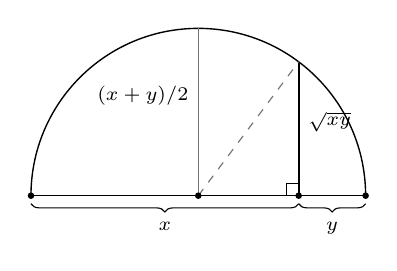
\begin{tikzpicture}[font=\scriptsize, scale=0.85]
\draw[line width=0.5pt] (5,0) arc[start angle=0, end angle=180, radius=2.5];
\draw[line width=0.5pt] (0,0) -- (5,0);
\draw[line width=0.8pt] (4,0) -- (4,2);
\draw[line width=0.5pt, black!55] (2.5,0) -- (2.5,2.5);
\draw[line width=0.4pt, black!55, dashed] (2.5,0) -- (4,2);
\fill (0,0) circle (1.4pt); \fill (4,0) circle (1.4pt); \fill (5,0) circle (1.4pt); \fill (2.5,0) circle (1.4pt);
\draw[decorate, decoration={brace, amplitude=3pt, mirror}] (0,-0.12) -- node[below=3pt] {$x$} (4,-0.12);
\draw[decorate, decoration={brace, amplitude=3pt, mirror}] (4,-0.12) -- node[below=3pt] {$y$} (5,-0.12);
\node[right] at (4,1.1) {$\sqrt{xy}$};
\node[left] at (2.5,1.5) {$(x+y)/2$};
\draw[line width=0.4pt] (3.82,0) -- (3.82,0.18) -- (4,0.18);
\end{tikzpicture}}{The inequality of the means for two numbers. On a diameter of length $x+y$, the radius (grey) is the arithmetic mean $(x+y)/2$. The perpendicular to the diameter at the point dividing it into $x$ and $y$ reaches the circle at height $\sqrt{xy}$, the geometric mean, by the theorem of Thales and similar triangles. A half-chord is never longer than the radius, and they are equal only when $x=y$.\label{fig:amgm}}
\end{figure}

A typical application is an optimisation without calculus. Among all boxes with given total edge length, which has the largest volume? If the edges are $a$, $b$ and $c$ with $a+b+c=s$ fixed, then $abc\le\bigl((a+b+c)/3\bigr)^3=(s/3)^3$, with equality exactly for the cube. Applied to the reciprocals $1/x_i$, the theorem also gives the \term{harmonic mean} inequality $n/(1/x_1+\cdots+1/x_n)\le G$.

\subsection{The Cauchy--Schwarz Inequality}

The next inequality bounds a sum of products by sums of squares. It is the most frequently used inequality in linear algebra, where $\sum a_ib_i$ is the inner product of two vectors (Part~III), and in statistics, where it shows that correlation coefficients lie between $-1$ and $1$ (Volume~III). Cauchy proved it for sums in 1821~\cite{cauchy1821}; the versions for integrals were found later by Bunyakovsky and by Schwarz~\cite{steele2004}.

\begin{theorem}[Cauchy--Schwarz inequality]
\label{thm:cauchy-schwarz}
For all real numbers $a_1,\ldots,a_n$ and $b_1,\ldots,b_n$,
\[
\Bigl(\sum_{i=1}^na_ib_i\Bigr)^2\le\Bigl(\sum_{i=1}^na_i^2\Bigr)\Bigl(\sum_{i=1}^nb_i^2\Bigr).
\]
Equality holds if and only if one of the tuples is a multiple of the other: $a_i=tb_i$ for all $i$, or $b_i=ta_i$ for all $i$, with one real $t$.
\end{theorem}

\begin{proof}
Write $A\coloneqq\sum a_i^2$, $B\coloneqq\sum b_i^2$ and $C\coloneqq\sum a_ib_i$. If $B=0$, then every $b_i=0$, both sides are $0$, and $b_i=0\cdot a_i$. Let $B>0$. For every real $t$,
\[
0\le\sum_{i=1}^n(a_i-tb_i)^2=A-2tC+t^2B ,
\]
a sum of squares. Choosing $t\coloneqq C/B$ gives $0\le A-2C^2/B+C^2/B=A-C^2/B$, that is, $C^2\le AB$. Equality holds if and only if $\sum(a_i-tb_i)^2=0$ for this $t$, that is, $a_i=tb_i$ for all $i$. Conversely, if $a_i=tb_i$ for all $i$, both sides equal $t^2B^2$, and the case $b_i=ta_i$ is symmetric.
\end{proof}

The proof is a miniature of a method used throughout this series: a quantity that is a sum of squares cannot be negative, and minimising it over a parameter turns this triviality into a sharp inequality. Two consequences are used often. Taking all $b_i=1$ gives
\[
\Bigl(\sum_{i=1}^na_i\Bigr)^2\le n\sum_{i=1}^na_i^2 ,
\]
which says that the arithmetic mean is at most the root mean square. And the Euclidean length $\|a\|\coloneqq\bigl(\sum a_i^2\bigr)^{1/2}$ of a tuple satisfies the triangle inequality
\begin{equation}
\|a+b\|\le\|a\|+\|b\| ,
\label{eq:minkowski}
\end{equation}
because $\|a+b\|^2=\|a\|^2+2\sum a_ib_i+\|b\|^2\le\|a\|^2+2\|a\|\,\|b\|+\|b\|^2=(\|a\|+\|b\|)^2$ by \cref{thm:cauchy-schwarz}. For $n=2$ this is the triangle inequality for complex numbers of \cref{prop:modulus}, read in the plane. Part~III develops both inequalities for vectors in $\mathbb R^n$ and $\mathbb C^n$.

\subsection{Products of Perturbations}

The last inequality of the chapter is a tool of rounding error analysis. In floating-point arithmetic every operation introduces a relative error: the computed result of an operation with exact result $x$ is $x(1+\delta)$ with $|\delta|\le u$, where $u$ is a small number called the unit roundoff, $u=2^{-53}\approx1.1\times10^{-16}$ for the binary64 format (Volume~V). After $n$ operations in sequence, factors $(1+\delta_1)\cdots(1+\delta_n)$ accumulate, and their effect must be bounded. In Higham's book on the accuracy of numerical algorithms, the following lemma is the basis of the analysis of sums, products and linear systems~\cite{higham2002accuracy}.

\begin{lemma}
\label{lem:gamma}
Let $u\ge0$ and $n\ge1$ with $nu<1$, and let $\delta_1,\ldots,\delta_n$ be real numbers with $|\delta_i|\le u$. Then
\[
\prod_{i=1}^n(1+\delta_i)=1+\theta_n\qquad\text{with}\qquad|\theta_n|\le\gamma_n\coloneqq\frac{nu}{1-nu}.
\]
\end{lemma}

\begin{proof}
We first show by induction on $n$ that $\bigl|\prod_{i=1}^n(1+\delta_i)-1\bigr|\le\prod_{i=1}^n(1+|\delta_i|)-1$. For $n=1$ both sides equal $|\delta_1|$. Write $P_n$ and $Q_n$ for the two products and suppose $|P_n-1|\le Q_n-1$. Since $P_{n+1}-1=(P_n-1)(1+\delta_{n+1})+\delta_{n+1}$,
\[
|P_{n+1}-1|\le|P_n-1|\,(1+|\delta_{n+1}|)+|\delta_{n+1}|\le(Q_n-1)(1+|\delta_{n+1}|)+|\delta_{n+1}|=Q_{n+1}-1 .
\]
Hence $|\theta_n|\le(1+u)^n-1$ by \cref{prop:ineq-rules}\,(ii). It remains to show $(1+u)^n\le1/(1-nu)$. Since $1/(1+u)\ge1-u$, which is equivalent to $1\ge1-u^2$, Bernoulli's inequality gives
\[
(1+u)^{-n}\ge(1-u)^n\ge1-nu>0 ,
\]
and taking reciprocals, $(1+u)^n\le1/(1-nu)$. Therefore $|\theta_n|\le1/(1-nu)-1=nu/(1-nu)$.
\end{proof}

For small $nu$ the bound $\gamma_n$ is only slightly larger than $nu$: the relative errors of $n$ operations add up, to first order, and their products contribute almost nothing. With $u=2^{-53}$ and a million operations, $nu\approx1.11\times10^{-10}$, and $\gamma_n$ agrees with $nu$ to ten significant digits. Volume~V uses the lemma to prove error bounds for the summation algorithms of the array library. It is a fitting end for this chapter: a statement about the fallible arithmetic of a computer, proved with nothing more than the axioms of an ordered field and an induction.

\section*{Notes}

The construction of the number systems from Peano's axioms is carried out in full, with every verification, in Landau's classic \emph{Grundlagen der Analysis}~\cite{landau1930}, and from a broader and more historical point of view in the collective volume \emph{Numbers} by Ebbinghaus and others~\cite{ebbinghaus1991}, which also covers the complex numbers, the fundamental theorem of algebra and the history of each system. Dedekind's two essays~\cite{dedekind1872,dedekind1888} are still readable and are the origin of the approach of \cref{sec:naturals,sec:reals}; Peano's axioms appeared in~\cite{peano1889}. The real numbers as a complete ordered field, including their uniqueness, are treated in the last part of Spivak's \emph{Calculus}~\cite{spivak2008calculus}, and the construction by Dedekind cuts in the appendix to the first chapter of Rudin~\cite{rudin1976}.

For the number theory of \cref{sec:division,sec:gcd,sec:primes,sec:congruences}, Hardy and Wright~\cite{hardywright2008} is the classic text, and Gauss's \emph{Disquisitiones Arithmeticae}~\cite{gauss1801} is the origin of the theory of congruences. Graham, Knuth and Patashnik~\cite{graham1994concrete} treat floor and ceiling functions and elementary number theory with an eye to computing. The second volume of Knuth's \emph{The Art of Computer Programming}~\cite{knuth1997taocp2} is the standard reference for the algorithmic side: positional number systems (Section~4.1), arbitrary-precision and modular arithmetic (Sections~4.3.1 and~4.3.2), the Euclidean algorithm and its analysis, including Lam\'e's theorem~\cite{lame1844} (Sections~4.5.2 and~4.5.3), and the evaluation of powers and polynomials (Sections~4.6.3 and~4.6.4). The conventions for integer division are compared by Boute~\cite{boute1992}.

Hardy, Littlewood and P\'olya~\cite{hardy1952inequalities} is the classic monograph on inequalities, and Steele~\cite{steele2004} a lively modern introduction centred on the Cauchy--Schwarz inequality. Higham~\cite{higham2002accuracy} shows how the elementary inequalities of \cref{sec:inequalities} become the error analysis of numerical algorithms, the subject of Volume~V.

\chapterreferences
